\documentclass[
	11pt,
	a4paper,
	oneside,
	cleardoubleempty, 
	idxtotoc,
	english,
	openright
	final,
	listof=nochaptergap,
	]{scrbook}
\usepackage{cmap}
\usepackage[T1]{fontenc}
\usepackage[utf8]{inputenc}
\usepackage{graphicx}

% ##################################################
% Unterstuetzung fuer die deutsche Sprache
% ##################################################
%\usepackage{ngerman}
\usepackage[ngerman, english]{babel}
\usepackage[UKenglish]{datetime}
\usepackage{graphicx}
\usepackage{wrapfig}

% ##################################################
% Dokumentvariablen
% ##################################################

% Persoenliche Daten
\newcommand{\docNachname}{Symhoven}
\newcommand{\docVorname}{Simon}
\newcommand{\docStrasse}{Boschetsriederstraße 59A}
\newcommand{\docOrt}{München}
\newcommand{\docPlz}{D-81379}
\newcommand{\docEmail}{simon.symhoven@hm.edu}
\newcommand{\docMatrikelnummer}{49651418}

\newcommand{\docFakultaet}{Fakultät Für Informatik und Mathematik}
\newcommand{\docSchwerpunkt}{SCHWERPUNKT}
\newcommand{\docInstitut}{INSTITUT}

% Dokumentdaten
\newcommand{\docTitle}{Interpretation linearer Modelle mit SHAP}
\newcommand{\docUntertitle}{Interpretation of linear models with SHAP}
% Arten der Arbeit: Bachelorthesis, Masterthesis, Seminararbeit, Diplomarbeit
\newcommand{\docArtDerArbeit}{Master-Thesis}
%Studiengaenge: Allgemeine Informatik Bachelor, Computer Networking Bachelor,
% Software-Produktmanagement Bachelor, Advanced Computer Scinece Master
\newcommand{\docStudiengang}{Stochastic Engineering in Business and Finance}
\newcommand{\docAbgabedatum}{\today}
\newcommand{\docErsterReferent}{Prof. Dr. Andreas Zielke}
\newcommand{\docZweiterReferent}{-} % Wenn es nur einen Betreuer gibt
%\newcommand{\docZweiterReferent}{Dr. Tobias Redele}

% ##################################################
% Allgemeine Pakete
% ##################################################

% Abbildungen einbinden
\usepackage{graphicx}

% Zusaetsliche Sonderzeichen
\usepackage{dingbat}

% Symbole Haken und X [OPTIONAL]
%\usepackage{pifont}
%\newcommand{\cmark}{\ding{51}}
%\newcommand{\xmark}{\ding{55}}

% Farben
\usepackage{color}
\usepackage[usenames,dvipsnames,svgnames,table]{xcolor}

% Maskierung von URLs und Dateipfaden
\usepackage[hyphens]{url}

% Deutsche Anfuehrungszeichen
\usepackage[babel, german=quotes]{csquotes}

% Pakte zur Index-Erstellung (Schlagwortverzeichnis)
\usepackage{index}
\makeindex

% AMS Packages
\usepackage{amsmath}
\usepackage{amsthm}
\usepackage{amssymb}

% Ipsum Lorem
% Paket wird nur für das Beispiel gebraucht und kann gelöscht werden
\usepackage{lipsum}

% ##################################################
% Seitenformatierung
% ##################################################
\usepackage[
	portrait,
	bindingoffset=1.5cm,
	inner=2.5cm,
	outer=3cm,
	top=3cm,
	bottom=2cm,
	%showframe, %Aktivieren um Seitengrenzen anzuzeigen
	%includeheadfoot
	]{geometry}

% ##################################################
% Kopf- und Fusszeile
% ##################################################

\usepackage{fancyhdr}

\pagestyle{fancy}
\fancyhf{}
\fancyhead[EL,OR]{\rmfamily\thepage}
\fancyhead[ER,OL]{\rmfamily\nouppercase{\leftmark}}

\fancypagestyle{headings}{}

\fancypagestyle{plain}{}

\fancypagestyle{empty}{
  \fancyhf{}
  \renewcommand{\headrulewidth}{0pt}
}

%Speichert \chaptermark in \oldchaptermark damit 
% es für die Anhänge zurückgesetzt werden kann
\let\oldchaptermark\chaptermark

%Kein "Kapitel # NAME" in der Kopfzeile
\renewcommand{\chaptermark}[1]{
	\markboth{#1}{}
   	\markboth{\thechapter.\ #1}{}
}

% ##################################################
% Schriften
% ##################################################

% Stdandardschrift festlegen
\renewcommand{\familydefault}{\rmdefault}

% Standard Zeilenabstand: 1,5 zeilig
\usepackage{setspace}
\onehalfspacing 

% Schriftgroessen festlegen
\addtokomafont{chapter}{\rmfamily\large\bfseries} 
\addtokomafont{section}{\rmfamily\normalsize\bfseries} 
\addtokomafont{subsection}{\rmfamily\normalsize\mdseries} 
\addtokomafont{caption}{\rmfamily\normalsize\mdseries} 

%Einrücken von Absätzen deaktivieren
\setlength{\parindent}{0pt}

%Zeilenabstand bei abstätzen
\usepackage{parskip}

% ##################################################
% Inhaltsverzeichnis / Allgemeine Verzeichniseinstellungen
% ##################################################

\usepackage{tocloft}

% Punkte auch bei Kapiteln
\renewcommand{\cftchapdotsep}{3}
\renewcommand{\cftdotsep}{3}

% Schriftart und -groesse im Inhaltsv erzeichnis anpassen
\renewcommand{\cftchapfont}{\rmfamily\normalsize}
\renewcommand{\cftsecfont}{\rmfamily\normalsize}
\renewcommand{\cftsubsecfont}{\rmfamily\normalsize}
\renewcommand{\cftchappagefont}{\rmfamily\normalsize}
\renewcommand{\cftsecpagefont}{\rmfamily\normalsize}
\renewcommand{\cftsubsecpagefont}{\rmfamily\normalsize}

%Zeilenabstand in den Verzeichnissen einstellen
\setlength{\cftparskip}{.5\baselineskip}
\setlength{\cftbeforechapskip}{.1\baselineskip}

%Einrücken von Absätzen deaktivieren
%\setlength{\parindent}{0pt}

%Zeilenabstand bei abstätzen
\usepackage{parskip}

% ##################################################
% Abbildungsverzeichnis und Abbildungen
% ##################################################

\usepackage{caption}

\usepackage{wrapfig}

% Nummerierung von Abbildungen
\renewcommand{\thefigure}{\arabic{figure}}
\usepackage{chngcntr}
\counterwithout{figure}{chapter}

% Abbildungsverzeichnis anpassen
\renewcommand{\cftfigpresnum}{Abbildung }
\renewcommand{\cftfigaftersnum}{:}

% Breite des Nummerierungsbereiches [Abbildung 1:]
\newlength{\figureLength}
\settowidth{\figureLength}{\bfseries\cftfigpresnum\cftfigaftersnum}
\addtolength{\figureLength}{2mm} %extra offset
\setlength{\cftfignumwidth}{\figureLength}
\setlength{\cftfigindent}{0cm}

% Schriftart anpassen
\renewcommand\cftfigfont{\rmfamily}
\renewcommand\cftfigpagefont{\rmfamily}

%standardpfad anpassen
\graphicspath{ {../src/content/pictures/} }

% ##################################################
% Tabellenverzeichnis und Tabellen
% ##################################################

% Nummerierung von Tabellen
\renewcommand{\thetable}{\arabic{table}}
\counterwithout{table}{chapter}

% Tabellenverzeichnis anpassen
\renewcommand{\cfttabpresnum}{Tabelle }
\renewcommand{\cfttabaftersnum}{:}

% Breite des Nummerierungsbereiches [Abbildung 1:]
\newlength{\tableLength}
\settowidth{\tableLength}{\bfseries\cfttabpresnum\cfttabaftersnum}
\addtolength{\tableLength}{3mm} %extra offset
\setlength{\cfttabnumwidth}{\tableLength}
\setlength{\cfttabindent}{0cm}

%Schriftart anpassen
\renewcommand\cfttabfont{\rmfamily}
\renewcommand\cfttabpagefont{\rmfamily}

% Unterdrueckung von vertikalen Linien
\usepackage{booktabs}

%Multi row für spezifische zellen
\usepackage{multirow}

%Additional table package
\usepackage{tabu}

% ##################################################
% Listings (Quellcode)
% ##################################################

\usepackage{listings}

%use typewriter font which supports bold characters
\usepackage{beramono}

\definecolor{codegreen}{rgb}{0,0.6,0}
\definecolor{codegray}{rgb}{0.5,0.5,0.5}
\definecolor{codepurple}{rgb}{0.5,0,0.33}
\definecolor{codepurblue}{rgb}{0.16,0.0,1.0}
\definecolor{backcolour}{rgb}{0.95,0.95,0.92}

\lstdefinestyle{codestyle}{
    backgroundcolor=\color{backcolour},   
    commentstyle=\color{codegreen},
    keywordstyle=\bfseries\color{codepurple},
    numberstyle=\tiny\color{codegray},
    stringstyle=\color{codepurblue},
    basicstyle=\scriptsize\ttfamily,
    breakatwhitespace=false,         
    breaklines=true,                 
    captionpos=b,                    
    keepspaces=true,                 
    numbers=left,                     
    numbersep=5pt,                 
    showspaces=false,                
    showstringspaces=false,
    showtabs=false,                  
    tabsize=2
}

\lstset{style=codestyle}

%Code auschnitt importieren aus datei
%\mylisting{from}{to}{language}{file}{descr}{path}
\newcommand{\mylisting}[6]{
\lstinputlisting[language=#3,
				firstnumber=#1,
				firstline=#1,
				lastline=#2,
				caption={#4, #5}, 
				label={implementation_listing_#4_#5}]
				{#6}
}

% ##################################################
% Appendix
% ##################################################

%Calc packet für berechnungen
\usepackage{calc}

%Appendix paket, setzen der flags für das TOC
\usepackage[toc,title,titletoc]{appendix} 

%Umbenennen der überschrift für die Anhänge 
\renewcommand{\appendixtocname}{Anhänge}

%Befehl für einen neuen Bericht und die erste seite als bild
\newcommand{\appendixsection}[2]{
\section{#1}
\appendixsingle{#2}
}

%Befehl für einzelne seite als bild eingefasst, damit überschrift und kopfzeile
% bestehen bleibt. 
\newcommand{\appendixsingle}[1]{
\vspace{-10cm}
\vfill
\mbox{}\hspace{-1.5cm}\includegraphics[width=\linewidth+3cm]{#1}\hspace{-1.5cm}\mbox{}
\vspace{-10cm}
\vfill
\mbox{}
}

%Datenträger Tabelle
\definecolor{lightgray}{gray}{0.85}
\definecolor{ultralightgray}{gray}{0.95}
\definecolor{mygray}{gray}{0.70}

% ##################################################
% Theoreme
% ##################################################
  	
% Umgebung fuer Beispiele
\newtheorem{beispiel}{Beispiel}

% Umgebung fuer These
\newtheorem{these}{These}

% Umgebung fuer Definitionen
\newtheorem{definition}{Definition}
  	
% ##################################################
% Literaturverzeichnis
% ##################################################

% ##################################################
% Abkuerzungsverzeichnis
% ##################################################

\usepackage[printonlyused]{acronym}

% ##################################################
% PDF / Dokumenteninternelinks
% ##################################################

\usepackage[
	colorlinks=false,
   	linkcolor=black,
   	citecolor=black,
  	filecolor=black,
	urlcolor=black,
    bookmarks=true,
    bookmarksopen=true,
    bookmarksopenlevel=3,
    bookmarksnumbered,
    plainpages=false,
    pdfpagelabels=true,
    hyperfootnotes,
    pdftitle ={\docTitle},
    pdfauthor={\docVorname~\docNachname},
    pdfcreator={\docVorname~\docNachname}]{hyperref}

% ####################################################
% Command für einfache QUellenangabe bei Bilder, etc.
% ####################################################

\newcommand{\source}[1]{\caption*{Quelle: {#1}} }



\begin{document}

\setcounter{secnumdepth}{3}

% Titelblatt
\begin{titlepage}
    \pagestyle{empty}
    
    \begin{center}	
    
    
\includegraphics[height=3cm]{content/pictures/hm.png}
    
    \vspace{1cm}

    \docFakultaet\\
    \docStudiengang\\

    \vspace{3cm}
    {\huge \docArtDerArbeit}\\

    \vspace{2cm}
    {\Huge \docTitle}\\
    \vspace{0.5cm}
    {\selectfont \docUntertitle}

    \vspace{2cm}
    Betreuer: \docErsterReferent\\
    %Co-Supervisor: \docZweiterReferent\\

    \end{center}

    \vspace{2cm}
    \begin{flushright}
    Eingereicht von: \\
    \docVorname~\docNachname, \docMatrikelnummer\\
    \docStrasse,~\docPlz~\docOrt\\
    \docEmail\\


    \vspace{0.7cm}
    \docOrt, den \today
    \end{flushright}

    \end{titlepage}
\cleardoubleemptypage

\frontmatter
\pagenumbering{roman}

% Abstract
\chapter*{Abstract\markboth{Abstract}{}}
\thispagestyle{empty}

In der vorliegenden Masterarbeit wird die Interpretation linearer Modelle mittels SHAP untersucht, 
einem Verfahren, das seine Grundlagen in den Shapley-Werten der kooperativen Spieltheorie findet. 
Die Untersuchung beginnt mit einem Rückblick auf die historische Entwicklung der Shapley-Werte und 
setzt sich mit einer detaillierten Herleitung sowie einer Analyse der zugrundeliegenden axiomatischen Prinzipien fort.
Es wird dargelegt, wie SHAP auf Basis der Shapley-Werte konzipiert wurde, um Beiträge der einzelnen Merkmale zur Vorhersagegenauigkeit 
eines Modells zu quantifizieren. 
Die Anwendung des Konzepts auf einen Datensatz aus der Praxis, bearbeitet mit dem Python-Paket \textsf{shap}, 
verdeutlicht die Handhabung und praktische Relevanz des Ansatzes. 
Den Schlussstein der Arbeit bildet ein Abgleich der gewonnenen Einsichten durch 
SHAP mit traditionellen Methoden zur Bestimmung der Relevanz von Modellmerkmalen. 
Zudem wird eine kritische Betrachtung der Grenzen und Herausforderungen, die SHAP mit sich bringt, präsentiert.
\cleardoubleemptypage

% Inhaltsverzeichnis 
\tableofcontents
\cleardoubleemptypage

\mainmatter

\chapter{Einleitung}

In einer Ära, in der datengetriebene Entscheidungsfindung und automatisierte Modelle zunehmend an Bedeutung gewinnen,
wird die Fähigkeit der Erklärung und Interpretation dieser Modelle immer wichtiger. Denn während maschinelles Lernen und
künstliche Intelligenz bedeutsame Fortschritte gemacht haben, bleiben viele Modelle aufgrund ihrer Komplexität und Undurchsichtigkeit
schwer verständlich. Die Frage, warum ein bestimmtes Modell eine entsprechende Entscheidung getroffen hat oder wie sich die einzelnen
Merkmale auf die Vorhersagen auswirken, wird zu einem zentralen Anliegen. 
Shapley-Werte bieten eine Möglichkeit, die \glqq{}Black Box\grqq{} der Modelle zu öffnen und Einblicke 
in die zugrunde liegenden Mechanismen zu gewinnen \cite[S. 3]{Molnar_2023}. 

Diese Masterarbeit widmet sich einer tiefgehenden Untersuchung der Shapley-Werte und erforscht ihr Potenzial für die Interpretation
von Machine Learning-Modellen, insbesondere linearer Modelle, sowie ihre Anwendbarkeit auf reale Datensätze.

Die Arbeit beginnt mit einer Einführung in die Shapley-Werte, indem ihre historischen Ursprünge 
und ihre Verbindung zur kooperativen Spieltheorie beleuchtet werden. Die theoretischen Grundlagen dieser Werte werden 
ergründet und ihre Bedeutung für die Interpretation von Modellen untersucht.

Anschließend wird der Fokus auf die Anpassung und Erweiterung der Shapley-Werte für maschinelles Lernen gelegt. 
Hierbei wird betrachtet, wie Shapley-Werte modifiziert werden können, um tiefere Einsichten in die Gewichtung 
und Bedeutung einzelner Merkmale innerhalb komplexer Machine Learning-Modelle zu ermöglichen. Dabei wird ein Vergleich 
mit bestehenden Methoden, wie der Permutation der Merkmalrelevanz, gezogen, wodurch die Einzigartigkeit und der Mehrwert der 
Shapley-Werte hervorgehoben wird.

Durch die Analyse eines realen Datensatzes wird die Methodik in der Praxis angewendet. Die Fallstudie zur Vorhersage der 
Druckfestigkeit von Beton bietet dabei ein konkretes Beispiel, anhand dessen die Nuancen und die Tiefe der durch SHAP 
ermöglichten Analysen veranschaulicht werden.

Abschließend werden die gewonnenen Erkenntnisse zusammengefasst und reflektiert. Es wird speziell die Rolle und das 
Potenzial der Shapley-Werte in diesem Kontext beleuchtet. Dabei werden schließlich die Grenzen und Herausforderungen, 
die mit der Anwendung von Shapley-Werten verbunden sind, kritisch diskutiert. 
\chapter{Hintergrund}


\section{Kooperative Spieltheorie}

Der Ursprung der Shapley Values liegt in der kooperativen Spieltheorie, einem fundamentalen Zweig der Spieltheorie. Dieser Bereich beschäftigt sich mit der Analyse von Situationen, in denen Akteure zusammenarbeiten, um gemeinsame Ziele zu erreichen. Zentrales Anliegen ist dabei die gerechte Verteilung der entstehenden Gewinne unter den Akteuren. Ein Schlüsselkonzept dieser Theorie ist die sogenannte "Charakteristische Funktion", welche die Bewertung der Gewinnverteilung einer Koalition von Akteuren ermöglicht.

Die Shapley Values, entwickelt von Lloyd Shapley in den 1950er Jahren, bieten einen methodischen Ansatz, um den individuellen Beitrag eines jeden Akteurs zur kooperativen Zusammenarbeit gerecht zu bewerten. Dies geschieht durch die Durchschnittsbewertung der Beiträge über sämtliche mögliche Koalitionen hinweg. Diese Methode erweist sich als äußerst nützlich, um eine gerechte und rationale Verteilung von Gewinnen in vielfältigen Szenarien zu ermöglichen, sei es in wirtschaftlichen Verhandlungen oder der Aufteilung von Ressourcen.

Das Verständnis der kooperativen Spieltheorie und ihrer Anwendung in Form der Shapley Values ermöglicht es, dieses theoretische Konzept auf den Bereich des maschinellen Lernens zu übertragen. In dieser Arbeit werden wir den Übergang von abstrakten Spieltheorie-Konzepten zu konkreten Anwendungen in der Welt der datengetriebenen Modelle erforschen.

Zur Erreichung dieses Ziels werden in den kommenden Abschnitten nicht nur die formalen Definitionen und Eigenschaften der Shapley Values erläutert, sondern auch ihre Adaption und Anwendung auf Machine Learning-Modelle in Betracht gezogen. Die Anwendbarkeit wird durch die praktische Anwendung auf einen realen Datensatz verdeutlicht.

\section{Formale Definition}

Sei $\mathcal{N} = \{1, \ldots, n\}$ eine endliche Spielermenge mit $n := |\mathcal{N}|$ Elementen. Sei $v$ die \textbf{Koalitionsfunktion}, die jeder Teilmenge von $\mathcal{N}$ eine reele Zahl zuweist und insbesondere der leeren Koalition den Wert $0$ gibt. 

\[
\begin{array}{rcccl}
  v &:  &\mathcal P(\mathcal{N}) &\longrightarrow &\mathbb{R}\\
  &: &v(\emptyset) &\mapsto &0\\
\end{array}
\]

Eine nicht leere Teilmenge der Spieler $\mathcal{S} \subseteq \mathcal{N}$ heißt Koalition. $\mathcal{N}$ selbst bezichnet die große Koalition. Den Ausdruck $v(\mathcal{S})$ nennt man den Wert der Koalition $\mathcal{S}$.
Der Shapley-Wert ordnet nun jedem Spieler aus $\mathcal{N}$ eine Auszahlung für das Spiel $v$ zu.

Der marginale Beitag eines Spieler $i \in N$, also der Wertbeitrag eines Spielers zu einer Koalition $\mathcal{S} \subseteq \mathcal{N}$, durch seinen Beitritt, ist

\begin{equation*}
v(\mathcal{S} \cup \{i\}) - v(\mathcal{S}).
\end{equation*}

Der Shapley-Wert eines Spielers $i$ errechnet sich als das gewichtete Mittel der marginalen Beiträge zu allen möglichen Koalitionen:

\begin{equation*}
\varphi_i (\mathcal{N}, v) = \sum_{\mathcal{S} \subseteq \mathcal{N} \setminus \{i\}} \underbrace{\frac{|\mathcal{S}|! \cdot (n - 1 - |\mathcal{S}|)!}{n!}}_{\text{Gewicht}} \underbrace{v(\mathcal{S} \cup \{i\}) - v(\mathcal{S})}_{\substack{\text{marginaler Beitrag von} \\ \text{Spieler $i$ zur Koalition $\mathcal{S}$}}}.
\end{equation*}

\section{Eigenschaften}

\paragraph{Pareto-Effizienz}

Der Wert der großen Koalition wird an die Spieler verteilt:

\begin{equation*}
\sum_{i \in \mathcal{N}} \varphi_i (\mathcal{N}, v) = v(\mathcal{N}).
\end{equation*}

\paragraph{Symmetrie}

Zwei Spieler $i$ und $j$, die die gleichen marginalen Beiträgen zu jeder Koalition haben,

\begin{equation*}
v(\mathcal{S} \cup \{i\}) = v(\mathcal{S} \cup \{j\})
\end{equation*}

erhalten das Gleiche:

\begin{equation*}
\varphi_i (\mathcal{N}, v) = \varphi_j (\mathcal{N}, v).
\end{equation*}

\paragraph{Null-Spieler-Eigenschaft}

Ein Spieler der zu jeder Koalition nichts bzw. den Wert seiner Einer-Koalition beiträgt, erhält null bzw. den Wert seiner Einer-Koalition:

\begin{equation*}
\varphi_i (\mathcal{N}, v) = 0,
\end{equation*}

bzw.

\begin{equation*}
\varphi_i (\mathcal{N}, v) = v(\{i\}).
\end{equation*}

\paragraph{Additivität}

Wenn das Spiel in zwei unabhängige Spiele zerlegt werden kann, dann ist die Auszahlung jedes Spielers im zusammengesetzten Spiel die Summe der Auszahlungen in den aufgeteilten Spielen:

\begin{equation*}
\varphi_i (\mathcal{N}, v + w) = \varphi_i (\mathcal{N}, v) + \varphi_i (\mathcal{N}, w).
\end{equation*}


\chapter{Theorie der Shapley-Werte}

Durch die Verwendung eines praktischen Beispiels – der Aufteilung 
eines Preisgeldes aus einem Designwettbewerb unter den Gewinnern – wird zunächst eine intuitive Einführung 
in das Konzept gegeben. Anschließend wird die formale Definition der Shapley-Werte erläutert, um die 
theoretischen Grundlagen für ihre Berechnung und Anwendung zu legen.

\section{Wie lässt sich der Gewinn gerecht aufteilen?}

Angenommen, drei Teilnehmer, Anna, Ben und Carla, haben als Team kooperiert und den ersten Platz bei einem Designwettbewerb belegt\footnote{In Anlehnung an das Beispiel aus Kapitel 4.1 \glqq{}Who's going to pay for that taxi?\grqq{} \cite[S.17-20]{Molnar_2023}.}. 
Dieser Erfolg führt zu einem Gesamtgewinn von 1000 \euro. Das Preisgeld für den zweiten Platz beträgt 750 \euro{} und 500 \euro{} für den dritten Platz.
Die Herausforderung besteht nun darin, den Gewinn auf eine Weise zu verteilen, die den individuellen Beitrag jedes Teilnehmers 
zur Erzielung des ersten Platzes gerecht widerspiegelt.

Die Situation wird komplizierter, wenn man bedenkt, dass jeder Teilnehmer unterschiedlich zu dem Erfolg 
beigetragen hat und ihre individuellen Leistungen auch zu verschiedenen Ausgängen geführt hätten, 
wenn sie alleine oder in anderen Teilkonstellationen angetreten wären.

Um eine faire Aufteilung des Preisgeldes zu erreichen, betrachten wir die hypothetischen Gewinne, 
die Anna, Ben und Carla erzielt hätten, wenn sie in unterschiedlichen Konstellationen am Wettbewerb teilgenommen hätten.
Tabelle \ref{tab:shapley_example} zeigt die gegebene Gewinnverteilung der verschiedenen Koalitionen. Die Koalition $\emptyset$ entspricht
dabei der leeren Koalition -- der Nichtteilnahme an dem Wettbewerb.

\begin{table}[!h]
  \caption{Potenzielle Gewinne für verschiedene Teilnehmerkonstellationen im\\Designwettbewerb.}
  \footnotesize
  \begin{tabularx}{\textwidth}{Xrr}
  \toprule
  Koalition & Gewinn & Bemerkung \\
  \midrule
  $\emptyset$ & 0 \euro & Keine Teilnahme \\
  $\{$Anna$\}$ & 500 \euro & 3. Platz als Einzelteilnehmerin \\
  $\{$Ben$\}$ & 750 \euro & 2. Platz als Einzelteilnehmer \\
  $\{$Carla$\}$ & 0 \euro & Kein Gewinn als Einzelteilnehmerin \\
  $\{$Anna, Ben$\}$ & 750 \euro & 2. Platz als Team ohne Carla \\
  $\{$Anna, Carla$\}$ & 750 \euro & 2. Platz als Team ohne Ben \\
  $\{$Ben, Carla$\}$ & 500 \euro & 3. Platz als Team ohne Anna \\
  $\{$Anna, Ben, Carla$\}$ & 1000 \euro & 1. Platz als Gesamtteam \\
  \bottomrule
  \end{tabularx}
  \label{tab:shapley_example}
  \normalsize\\
  Quelle: Eigene Darstellung.
\end{table}

Zur Berechnung der Shapley-Werte ist es erforderlich, den marginalen Beitrag jedes Spielers zu erfassen.
Marginalbeiträge in der Spieltheorie, und speziell im Kontext der Shapley-Werte, sind die zusätzlichen Beiträge, 
die ein Spieler (Teilnehmer) zum Gesamtgewinn einer Koalition beiträgt, wenn er dieser beitritt. 
Die Berechnung des marginalen Beitrags eines Teilnehmers erfolgt, indem man den Wert der Koalition ohne diesen Teilnehmer 
vom Wert der Koalition mit dem Teilnehmer subtrahiert \cite[S. 18]{Molnar_2023}.

In diesem Beispiel mit Anna, Ben und Carla, die an einem Designwettbewerb teilnehmen, ist der marginale Beitrag von 
Anna zur Koalition von $\{$Ben$\}$ der zusätzliche Wert, den Anna einbringt, wenn sie sich Ben anschließt, 
ausgehend von Bens individuellem Gewinn.

\begin{table}[!h]
  \caption{Marginalbeiträge der einzelnen Teilnehmer zu den möglichen Koalitionen.}
  \footnotesize
  \begin{tabularx}{\textwidth}{XXrrr}
  \toprule
  Teilnehmer & Zur Koalition & Gewinn vorher & Gewinn nachher & Marginalbeitrag \\
  \midrule
  Anna & $\emptyset$ & 0 \euro & 500 \euro & 500 \euro \\
  Anna & $\{$Ben$\}$ & 750 \euro & 750 \euro & 0 \euro \\
  Anna & $\{$Carla$\}$ & 0 \euro & 750 \euro & 750 \euro \\
  Anna & $\{$Ben, Carla$\}$ & 500 \euro & 1000 \euro & 500 \euro\\
  Ben & $\emptyset$ & 0 \euro & 750 \euro & 750 \euro \\
  Ben & $\{$Anna$\}$ & 500 \euro & 750 \euro & 250 \euro\\
  Ben & $\{$Carla$\}$ & 0 \euro & 500 \euro & 500 \euro\\
  Ben & $\{$Anna, Carla$\}$ & 750 \euro &  1000 \euro & 250 \euro\\
  Carla & $\emptyset$ & 0 \euro & 0 \euro & 0 \euro \\
  Carla & $\{$Anna$\}$ & 500 \euro & 750 \euro & 250 \euro \\
  Carla & $\{$Ben$\}$ & 750 \euro & 500 \euro & -250 \euro \\
  Carla & $\{$Anna, Ben$\}$ & 750 \euro & 1000 \euro & 250 \euro \\
  \bottomrule
  \end{tabularx}
  \label{tab:shapley_marginal}
  \normalsize\\
  Quelle: Eigene Darstellung.
\end{table}

Tabelle \ref{tab:shapley_marginal} illustriert den Gewinn jeder möglichen Koalition ohne den 
betrachteten Spieler und den neuen Gesamtgewinn, sobald dieser Spieler der Koalition beitritt. 
Der marginale Beitrag jedes Spielers wird als Differenz zwischen diesen beiden Werten 
berechnet und gibt Aufschluss über den individuellen Wertbeitrag zum gemeinschaftlichen Erfolg.

Nachdem die marginalen Beiträge jedes Teilnehmers für die verschiedenen Koalitionen festgestellt wurden, 
ist der nächste Schritt, die Shapley-Werte zu bestimmen, welche eine faire Aufteilung des Gesamtgewinns 
erlauben. Hierzu wird jede mögliche Permutation betrachtet, in der die Spieler der 
Koalition beitreten könnten. Jede dieser Permutationen liefert unterschiedliche marginale Beiträge 
für die Spieler, je nach der Reihenfolge ihres Beitritts, wie Tabelle \ref{tab:shapley_marginal} zeigt \cite[S. 19]{Molnar_2023}.

Im Falle des Beispiels mit Anna, Ben und Carla bedeutet dies, dass alle möglichen Reihenfolgen 
berücksichtigt werden müssen, in denen sie zum ersten Platz beigetragen haben könnten. 
Die Shapley-Werte werden als Durchschnitt der marginalen Beiträge über alle Permutationen berechnet. 
Dies gewährleistet, dass jeder Spieler einen Anteil des Preisgeldes erhält, der seinem durchschnittlichen 
Beitrag zum Erfolg entspricht \cite[S. 20]{Molnar_2023}.

Bei drei Teilnehmern exisitieren $3! = 3 \cdot 2 \cdot 1 = 6$ Permutationen:

\begin{enumerate}[itemsep=0pt, parsep=0pt]
  \item Anna, Ben, Carla
  \item Anna, Carla, Ben
  \item Ben, Anna, Carla
  \item Carla, Anna, Ben
  \item Ben, Carla, Anna
  \item Carla, Ben, Anna
\end{enumerate}

Jede Permutation entspricht einer Koalitionsbildung. Anna wird in zwei Koalitionsbildungen (1. und 2.) einer leeren Koalition hinzugefügt, da Sie die erste ist, 
die der Koalition beitritt.
In weiteren zwei Koalitionsbildungen (5. und 6.) wird Anna der bestehenden Koalition aus Ben und Carla, respektive Carla und Ben hinzugefügt. 
In den beiden übrigen Koalitionsbildungen wird Anna einmal der Koaliton bestehend aus Ben (3.) und einmal der Koalition bestehend aus Carla (4.)
hinzugefügt. 

Zusammen mit Tabelle \ref{tab:shapley_marginal} lässt sich nun der Shapley-Wert mit den gewichteten durchschnittlichen marginalen Beiträge für Anna berechnen:

\begin{equation}
  \frac{1}{6} ( \underbrace{2 \cdot 500 \text{\euro}}_{\text{A $\rightarrow$ $\{\emptyset$\}}} + \underbrace{1 \cdot 0 \text{\euro}}_{\text{A $\rightarrow$ $\{B$\}}} + \underbrace{1 \cdot 750 \text{\euro}}_{\text{A $\rightarrow$ $\{C$\}}} + \underbrace{2 \cdot 500 \text{\euro}}_{\text{A $\rightarrow$ $\{B, C$\}}} ) \approx 458,33 \text{\euro}.  
\label{eq:marginal_anna}
\end{equation}

Analog gilt dies für Ben:

\begin{equation}
  \frac{1}{6} ( \underbrace{2 \cdot 750 \text{\euro}}_{\text{B $\rightarrow$ $\{\emptyset$\}}} + \underbrace{1 \cdot 250 \text{\euro}}_{\text{B $\rightarrow$ $\{A$\}}} + \underbrace{1 \cdot 500 \text{\euro}}_{\text{B $\rightarrow$ $\{C$\}}} + \underbrace{2 \cdot 250 \text{\euro}}_{\text{B $\rightarrow$ $\{A, C$\}}} ) \approx 458,33 \text{\euro},  
  \label{eq:marginal_ben}
\end{equation}

und Carla:

\begin{equation}
  \frac{1}{6} ( \underbrace{2 \cdot 0 \text{\euro}}_{\text{C $\rightarrow$ $\{\emptyset$\}}} + \underbrace{1 \cdot 250 \text{\euro}}_{\text{C $\rightarrow$ $\{A$\}}} + \underbrace{1 \cdot (-250) \text{\euro}}_{\text{C $\rightarrow$ $\{B$\}}} + \underbrace{2 \cdot 250 \text{\euro}}_{\text{C $\rightarrow$ $\{A, B$\}}} ) \approx 83,33 \text{\euro}  
  \label{eq:marginal_carla}
\end{equation}

Auf Basis der gewichteten durchschnittlichen marginalen Beiträge lässt sich feststellen, 
dass Anna und Ben jeweils einen Shapley-Wert von ungefähr 458,33 \euro{} erhalten, 
während Carla einen Shapley-Wert von etwa 83,33 \euro{} zugewiesen bekommt. 
Diese Werte spiegeln den fairen Anteil jedes Teilnehmers an der Gesamtprämie wider, 
basierend auf ihrem individuellen Beitrag zum Erfolg des Teams \cite[S. 20]{Molnar_2023}. Mit dieser konkreten Anwendung der Shapley-Werte 
auf ein alltagsnahes Beispiel wird nun die zugrunde liegende Theorie und die formale Definition 
der Shapley-Werte, die diese Berechnungen ermöglichen, detaillierter betrachtet.

\section{Formale Definition}

Sei $\mathcal{N} = \{1, \ldots, n\}$ eine endliche Spielermenge mit $n := |\mathcal{N}|$ Elementen. Sei $v$ die Koalitionsfunktion, die jeder Teilmenge von $\mathcal{N}$ eine reelle Zahl zuweist und insbesondere der leeren Koalition den Wert $0$ gibt. 

\[
\begin{array}{rcccl}
  v &:  &\mathcal P(\mathcal{N}) &\longrightarrow &\mathbb{R}\\
  &: &v(\emptyset) &\mapsto &0\\
\end{array}
\]

Eine nicht leere Teilmenge der Spieler $\mathcal{S} \subseteq \mathcal{N}$ heißt Koalition. $\mathcal{N}$ selbst bezeichnet die große Koalition. Den Ausdruck $v(\mathcal{S})$ nennt man den Wert der Koalition $\mathcal{S}$.
Der Shapley-Wert ordnet nun jedem Spieler aus $\mathcal{N}$ eine Auszahlung für das Spiel $v$ zu.

Der marginale Beitag eines Spielers $i \in \mathcal{N}$, also der Wertbeitrag eines Spielers zu einer Koalition $\mathcal{S} \subseteq \mathcal{N}$, durch seinen Beitritt, ist

\begin{equation}
v(\mathcal{S} \cup \{i\}) - v(\mathcal{S}).
\label{eq:marignal}
\end{equation}


Sei $i = \text{Anna}$ und $\mathcal{S} = \{\text{Ben}\}$, dann ist $v(\mathcal{\{\text{Ben}\}} \cup \{\text{Anna}\}) - v(\mathcal{\{\text{Ben}\}})$ das
zusätzliche Preisgeld, welches gewonnen wird, wenn Anna der Koalition mit Ben beitritt. 


Der Shapley-Wert eines Spielers $i$ errechnet sich als das gewichtete Mittel der marginalen Beiträge zu allen möglichen Koalitionen:

\begin{equation}
\varphi_i (\mathcal{N}, v) = \sum_{\mathcal{S} \subseteq \mathcal{N} \setminus \{i\}} \underbrace{\frac{|\mathcal{S}|! \cdot (n - 1 - |\mathcal{S}|)!}{n!}}_{\text{Gewicht}} \underbrace{v(\mathcal{S} \cup \{i\}) - v(\mathcal{S})}_{\substack{\text{marginaler Beitrag von} \\ \text{Spieler $i$ zur Koalition $\mathcal{S}$}}}.
\end{equation}

Die Summationsnotation \(\sum_{\mathcal{S} \subseteq \mathcal{N} \setminus \{i\}}\) erfasst die marginalen Beiträge, 
die der Spieler \( i \) zu allen Koalitionen leistet, welche diesen noch nicht einschließen. Die Verwendung von 
\(\mathcal{N} \setminus \{i\}\) stellt sicher, dass Spieler \( i \) nur für jene Koalitionen berücksichtigt wird, 
zu denen er noch beitragen kann. Im Falle von Anna etwa, beziehen sich die Berechnungen auf die Koalitionen bestehend 
aus der leeren Koalition \(\emptyset\), aus \(\{\text{Ben}\}\), \(\{\text{Carla}\}\), oder beiden 
zusammen \(\{\text{Ben, Carla}\}\) (vgl. Berechnung \ref{eq:marginal_anna}).

Die Formel \(\frac{|\mathcal{S}|! \cdot (n - 1 - |\mathcal{S}|)!}{n!}\) in der Shapley-Wert-Berechnung 
reflektiert den Gewichtungsfaktor für die marginalen Beiträge eines Spielers. Hierbei gibt \(|\mathcal{S}|!\) die Permutationen 
der Spieler innerhalb der Koalition \(\mathcal{S}\) an, während \((n - 1 - |\mathcal{S}|)!\) die Anordnungen der 
außenstehenden Spieler repräsentiert, nachdem der betrachtete Spieler beigetreten ist. 
Der Bruchteil \(\frac{1}{n!}\) normalisiert diesen Wert über alle möglichen Koalitionszusammensetzungen, 
wodurch die Wahrscheinlichkeit der Bildung einer spezifischen Koalition ausgedrückt wird.

Betrachten wir Anna als den Spieler $i$ und die Koalition \(\mathcal{S} = \{\text{Ben, Carla}\}\). 
Die Formel \(\frac{|\mathcal{S}|! \cdot (n - 1 - |\mathcal{S}|)!}{n!}\) berechnet den Gewichtungsfaktor 
für Annas marginalen Beitrag zur Koalition \(\mathcal{S}\). In diesem Fall ist \(|\mathcal{S}| = 2\) und \(n = 3\). 
Somit ergibt sich \(|\mathcal{S}|! = 2!\) und \(n - 1 - |\mathcal{S}| = 0!\), da nach dem Beitritt von 
Anna keine weiteren Spieler übrig sind. Der Normalisierungsfaktor ist \(n! = 3! = 6\). Daraus folgt:

\begin{equation}
\frac{2! \cdot 0!}{3!} = \frac{2 \cdot 1}{6} = \frac{1}{3}.
\end{equation}

Dies bedeutet, dass unter allen möglichen Permutationen der Spielerreihenfolge, Annas Beitritt zu der Koalition \{Ben, Carla\} 
in genau ein Drittel der Fälle geschieht. Somit wird ihr marginaler Beitrag mit diesem Faktor gewichtet, 
um den Shapley-Wert zu berechnen (vgl. Berechnung \ref{eq:marginal_anna}) \cite[S. 21f]{Molnar_2023}.


\section{Axiomatische Grundlage}
\label{sec:axiome-shapley}

Nachdem die Berechnung des Shapley-Werts für das Beispiel konkretisiert wurde, ist es nun von Bedeutung, die zugrundeliegenden Axiome zu betrachten, 
welche die theoretische Rechtfertigung für die Methode liefern. Der Shapley-Wert wird nicht nur durch seine Berechnungsmethode, 
sondern auch durch eine Reihe von Axiomen charakterisiert, die seine Fairness und Kohärenz im Kontext kooperativer Spiele sicherstellen. 
Lloyd Shapley leitete den Shapley-Wert ursprünglich aus diesen Axiomen ab und bewies, 
dass dieser der einzige ist, der den Axiomen genügt\footnote{Eine detaillierte Darstellung dieser Axiome und des Beweises 
ihrer Einzigartigkeit findet sich in Shapleys Originalarbeit, deren umfassende Behandlung jedoch den Rahmen dieser Arbeit überschreiten würde \cite[S. 307-318]{Shapley+1953+307+318}.}. 
Diese Axiome sind wesentliche Bestandteile, die die Einzigartigkeit und die wünschenswerten Eigenschaften des Shapley-Werts als Lösungskonzept definieren \cite[S. 22]{Molnar_2023}. 

\paragraph{Effizienz}

Der Wert der großen Koalition wird an die Spieler verteilt:

\begin{equation}
\sum_{i \in \mathcal{N}} \varphi_i (\mathcal{N}, v) = v(\mathcal{N}).
\end{equation}

Dies bedeutet, dass die Summe der Shapley-Werte aller Spieler dem Gesamtwert entspricht, 
den die Koalition aller Spieler zusammen erreichen kann. Der Gesamtwert, den die große Koalition $\mathcal{N}$, 
bestehend aus Anna, Ben und Carla, generiert, wird komplett unter den Spielern aufgeteilt \cite[S. 22]{Molnar_2023}. 
Unter Vernachlässigung minimaler Rundungsdifferenzen entspricht die Summe der Shapley-Werte, 
berechnet in den Gleichungen \ref{eq:marginal_anna}, \ref{eq:marginal_ben} und \ref{eq:marginal_carla}, 
dem kollektiven Ertrag der großen Koalition:

\begin{equation}
  458,33 \text{\euro} + 458,33 \text{\euro} + 83,33 \text{\euro} \approx 1000 \text{\euro} 
\end{equation}


\paragraph{Symmetrie}

Zwei Spieler $i$ und $j$, die die gleichen marginalen Beiträgen zu jeder Koalition haben, bekommen den gleichen Wert
zugewiesen:

\begin{equation}
v(\mathcal{S} \cup \{i\}) = v(\mathcal{S} \cup \{j\}), \; \forall\, \mathcal{S} \subseteq \mathcal{N} \setminus \{i, j\} \Rightarrow \varphi_i (\mathcal{N}, v) = \varphi_j (\mathcal{N}, v).
\end{equation}

Obwohl Anna und Ben den gleichen Shapley-Wert erhalten, ist dies nicht auf das Symmetrieaxiom zurückzuführen, 
da ihre marginalen Beiträge zu den Koalitionen variieren. Zum Beispiel leistet Anna keinen Beitrag zur Koalition, 
wenn Ben bereits Teil davon ist, während Ben einen positiven Beitrag leistet, 
wenn Anna bereits zur Koalition gehört (vgl. Tabelle \ref{tab:shapley_marginal}). Dies zeigt, dass die Gleichheit ihrer Shapley-Werte ein Ergebnis der 
spezifischen Zahlenkonstellation in diesem Szenario ist und nicht aus der symmetrischen Interaktion 
zwischen den beiden Spielern resultiert.

\paragraph{Null-Spieler-Eigenschaft (Dummy-Spieler-Eigenschaft)}

Ein Spieler $i$, der zu jeder Koalition nichts beiträgt, erhält den Wert Null:

\begin{equation}
  v(\mathcal{S} \cup \{i\}) =  v(\mathcal{S}), \; \forall\, \mathcal{S} \subseteq \mathcal{N} \setminus \{i\} \Rightarrow \varphi_i (\mathcal{N}, v) = 0.
\end{equation}

Dies stell sicher, dass ein Spieler, der keinen Beitrag leistet, auch nicht belohnt wird. 

\paragraph{Additivität} 

Wenn das Spiel in zwei unabhängige Spiele mit Koalitionsfunktionen $v$ und $w$ zerlegt werden kann, dann ist die Auszahlung jedes Spielers im 
zusammengesetzten Spiel die Summe der Auszahlungen in den aufgeteilten Spielen:

\begin{equation}
\varphi_i (\mathcal{N}, v + w) = \varphi_i (\mathcal{N}, v) + \varphi_i (\mathcal{N}, w).
\end{equation}

Wenn Anna, Ben und Carla neben dem ersten Wettbewerb an einem zweiten, unabhängigen Wettbewerb teilnehmen, 
besagt das Additivitätsaxiom, dass die Shapley-Werte jedes Spielers aus beiden Wettbewerben einfach die Summe ihrer individuellen 
Shapley-Werte aus jedem einzelnen Wettbewerb sind. Dies impliziert, dass die faire Aufteilung der Gewinne aus beiden Wettbewerben 
konsistent bleibt, indem die aus dem ersten Wettbewerb abgeleiteten Prinzipien auf den zweiten Wettbewerb übertragen und 
dann addiert werden \cite[S. 5573, S.22f]{ijcai2022p778, Molnar_2022}.
\chapter{Von Shapley-Werten zu SHAP: Brückenschlag zur Modellinterpretation}

Im Rahmen der kooperativen Spieltheorie ermöglichen die Shapley-Werte eine faire Verteilung des kollektiv 
erwirtschafteten Nutzens auf die beteiligten Akteure. Diese Methodik findet eine analoge Anwendung 
in der Welt des maschinellen Lernens, um die Beiträge einzelner Merkmale zur Vorhersageleistung 
eines Modells zu bewerten. Hier wird die Terminologie der Shapley-Werte in den Kontext von Machine Learning 
Modellen übertragen, wobei jedes Merkmal als \glqq{}Spieler\grqq{} betrachtet wird, dessen Beitrag zur 
\glqq{}Auszahlung\grqq{} – der Vorhersage des Modells – evaluiert werden soll. 

\begin{table}[!h]
    \caption{Terminologie der originären Shapley-Werte im Kontext des maschinellen Lernens.}
    \footnotesize
    \begin{tabularx}{\textwidth}{XXX}
    \toprule
    Terminologie Konzept & Terminologie Machine Learning & Ausdruck \\
    \midrule
    Spieler & Merkmal Index & $j$ \\
    Anzahl aller Spieler & Anzahl aller Merkmale & $p$ \\
    Große Koalition & Menge aller Merkmale & $\mathcal{N} = \{1, \ldots, p\}$\\
    Koalition & Menge von Merkmalen & $\mathcal{S} \subseteq \mathcal{N}$ \\
    Größe der Koalition & Anzahl der Merkmale in der Koalition $\mathcal{S}$ & $|\mathcal{S}|$\\
    Spieler, die nicht in der Koalition sind & Merkmale, die nicht in der Koalition enthalten sind & $C: C = \mathcal{N} \setminus \mathcal{S}$ \\
    Koalitionsfunktion & Vorhersage für Merkmalswerte in der Koalition $\mathcal{S}$ abzüglich der Vorhersage im Mittel & $v_{f, x^{(i)}}(\mathcal{S}$)\\
    Auszahlung & Vorhersage für eine Beobachtung $x^{(i)}$ abzüglich der Vorhersage im Mittel & $f(x^{(i)}) -  \mathbb{E}(f(X))$\\
    Shapley-Wert & Beitrag des Merkmals $j$ zur Auszahlung des Modells für eine Beobachtung $x^{(i)}$& $\varphi_j^{(i)}(\mathcal{N}, f)$\\
    \bottomrule
    \end{tabularx}
    \label{tab:shapley_terms}
    \normalsize\\
    Quelle: \cite[S. 26]{Molnar_2023}.
\end{table}

Die Koalitionsfunktion $v_{f, x^{(i)}}(\mathcal{S})$ für ein gegebenes Model $f$ und eine Beobachtung $x^{(i)}$ ist definiert als:

\begin{align}
    \label{eq:shap-value-func}
    v_{f, x^{(i)}}(\mathcal{S}) = \int_{\mathbb{R}} f(x^{(i)}_{\mathcal{S}} \cup X_{C}) d\mathbb{P}_{X_{C}} - \mathbb{E}(f(X))
\end{align}

Diese Funktion berechnet den erwarteten Wert der Vorhersage des Modells $f$, wenn nur eine Teilmenge $\mathcal{S}$ der 
Merkmale genutzt wird, um die Vorhersage für die spezifische Beobachtung $x^{(i)} \in \mathbb{R}^{p}$ zu treffen. 
Das Integral $\int_{\mathbb{R}}$ repräsentiert die Berechnung dieses erwarteten Wertes über alle möglichen Werte der Merkmale, 
die nicht in $\mathcal{S}$ enthalten sind ($X_C$), gewichtet durch deren Wahrscheinlichkeitsverteilung $\mathbb{P}_{X_{C}}$. 
Die Differenz zum Erwartungswert der Vorhersagen über alle Merkmale $\mathbb{E}(f(X))$ zeigt, 
wie viel die spezifische Menge an Merkmalen $\mathcal{S}$ zur Vorhersage beiträgt \cite[S. 221, S. 27]{Molnar_2022, Molnar_2023}.

Der marginale Beitrag eines Merkmals $j$ zu einer Koalition $\mathcal{S}$ ist dann:

\begin{align}
    \label{eq:shap-marginal-func}
    v_{f, x^{(i)}}(\mathcal{S} \cup \{j\}) - v_{f, x^{(i)}}(\mathcal{S}) &= \int_{\mathbb{R}} f(x^{(i)}_{\mathcal{S} \cup \{j\}} \cup X_{C \setminus \{j\}}) d\mathbb{P}_{X_{C \setminus \{j\}}} - \mathbb{E}(f(X)) \\ \notag
    &\quad - \left( \int_{\mathbb{R}} f(x^{(i)}_{\mathcal{S}} \cup X_{C}) d\mathbb{P}_{X_{C}} - \mathbb{E}(f(X)) \right) \\ \notag
    &= \int_{\mathbb{R}} f(x^{(i)}_{\mathcal{S} \cup \{j\}} \cup X_{C \setminus \{j\}}) d\mathbb{P}_{X_{C \setminus \{j\}}} \\ \notag
    &\quad - \int_{\mathbb{R}} f(x^{(i)}_{\mathcal{S}} \cup X_{C}) d\mathbb{P}_{X_{C}}
\end{align}

Diese Gleichung beschreibt, wie sich der erwartete Wert der Vorhersage ändert, wenn das Merkmal $j$ zu der Menge der Merkmale $\mathcal{S}$ hinzugefügt wird \cite[S. 29]{Molnar_2023}.

Der Beitrag $\varphi_j^{(i)}(\mathcal{N}, f)$ eines Merkmals $j$ für eine Beobachtung $x^{(i)} \in \mathbb{R}^{p}$ für die Vorhersage $f(x^{(i)})$ ist gegeben als:

\begin{align}
    \label{eq:shap-eq}
    \varphi^{(i)}_{j} (\mathcal{N}, f) &= \sum_{\mathcal{S} \subseteq \mathcal{N} \setminus \{j\}} \frac{|\mathcal{S}|! \cdot (p - 1 - |\mathcal{S}|)!}{p!} \\ \notag
    &\quad \cdot \left( \int_{\mathbb{R}} f(x^{(i)}_{\mathcal{S} \cup \{j\}} \cup X_{C \setminus \{j\}}) d\mathbb{P}_{X_{C \setminus \{j\}}} -
    \int_{\mathbb{R}} f(x^{(i)}_{\mathcal{S}} \cup X_{C}) d\mathbb{P}_{X_{C}} \right) 
\end{align}

Diese Formel ist die zentrale Berechnung der SHAP-Werte im maschinellen Lernen. 
Sie summiert den gewichteten, marginalen Beitrag des Merkmals $j$ über alle möglichen Kombinationen der anderen Merkmale. 
Die Gewichtung berücksichtigt die Anzahl der Merkmale in der Koalition $\mathcal{S}$ und die Anzahl der verbleibenden Merkmale, 
die noch hinzugefügt werden können. Dies ergibt den durchschnittlichen Beitrag des Merkmals $j$ zur Vorhersage für die 
Beobachtung $x^{(i)}$ \cite[S. 29, 30]{Molnar_2023}.

Die Integration in der SHAP-Formel ist ein zentraler Schritt, um den erwarteten Beitrag jedes Merkmals unter 
Berücksichtigung der gesamten Verteilung der Daten zu ermitteln. 
In diesem Ansatz werden die Merkmale als Zufallsvariablen behandelt, und die Integration erfolgt über 
die Wahrscheinlichkeitsverteilungen dieser Zufallsvariablen. Durch das Berechnen der erwarteten Vorhersagewerte mit 
und ohne des jeweiligen Merkmals, unter Einbeziehung der Verteilung aller anderen Merkmale, 
ermöglicht SHAP eine präzise und umfassende Einschätzung des Einflusses jedes einzelnen Merkmals. 
Dieser Prozess der Marginalisierung, bei dem man über die Wahrscheinlichkeitsverteilungen der Merkmale integriert, 
erlaubt es, den Beitrag eines jeden Merkmals zu isolieren und unabhängig von der spezifischen Zusammensetzung 
der anderen Merkmale zu bewerten. Dies führt zu einer fairen und ganzheitlichen Bewertung der Beiträge aller Merkmale 
zur Vorhersage des Modells \cite[S. 28]{Molnar_2023}.

\section{Berechnung der SHAP-Werte unter Berücksichtigung der zugrundeliegenden Verteilung}
\label{sec:example}

Ein einfaches Beispiel soll helfen, die Anwendung von SHAP-Werten im 
Kontext des maschinellen Lernens zu illustrieren\footnote{In Anlehnung an das Beispiel aus Kapitel 8.5.1 \glqq{}General Idea\grqq{} \cite[S.215f]{Molnar_2022}.}. Betrachtet wird ein fiktiver 
Immobilien-Datensatz mit drei Merkmalen: Größe des Hauses in Quadratmetern ($x_1$), Anzahl der Zimmer ($x_2$) 
und Entfernung zum Stadtzentrum in Kilometern ($x_3$). Es gibt zwei Beobachtungen in diesem Datensatz:

\begin{table}[!h]
    \caption{Merkmale von Beobachtungen in einem Immobilien-Datensatz.}
    \footnotesize
    \begin{tabularx}{\textwidth}{Xrrr}
    \toprule
     & $x_1$: Größe (in $m^2$) &  $x_2$: Anzahl Zimmer &  $x_3$: Entfernung zum Zentrum (in km) \\
    \midrule
    $x^{(1)}$ & 100 & 3 & 5 \\
    $x^{(2)}$ & 150 & 4 & 10 \\
    \bottomrule
    \end{tabularx}
    \label{tab:example}
    \normalsize\\
    Quelle: Eigene Darstellung.
\end{table}

Angenommen das Modell $f(x^{(i)})$ prognostiziert den Preis eines Hauses in Euro als eine lineare Kombination der Merkmale:

\begin{equation}
    f(x^{(i)}) = 5x_1^{(i)} + 20x_2^{(i)} - 2x_3^{(i)}.
\end{equation}

Die Vorhersagen für die beiden Beobachtungen lauten dann:

\begin{align}
    \label{eq:fx1}
    f(x^{(1)}) &= 5x_1^{(1)} + 20x_2^{(1)} - 2x_3^{(1)} \\ \notag
        &= 5 \cdot 100 + 20 \cdot 3 - 2 \cdot 5 \\ \notag
        &= 550\,\text{\euro} 
\end{align}

und 

\begin{align}
    f(x^{(2)}) &= 5x_1^{(2)} + 20x_2^{(2)} - 2x_3^{(2)} \\ \notag
        &= 5 \cdot 150 + 20 \cdot 4 - 2 \cdot 10 \\ \notag
        &= 810\,\text{\euro}. 
\end{align}

Die erwartete Auszahlung des Modells $\mathbb{E}(f(X))$ wird berechnet als:
\begin{align}
    \label{eq:efx}
    \mathbb{E}(f(X)) &= 5 \cdot \mathbb{E}(X_1) + 20 \cdot \mathbb{E}(X_2) - 2 \cdot \mathbb{E}(X_3) \\ \notag
                     &= 5 \cdot 125 + 20 \cdot 3,5 - 2 \cdot 7,5 \\ \notag
                     &= 680 \,\text{\euro},
\end{align}

mit 

\begin{align}
    \label{eq:e}
    \mathbb{E}(X_j) = \frac{1}{n} \sum_{i=1}^{n} x_j^{(i)}.
\end{align}     

Sei $\mathcal{N} = \{1, 2, 3\}$ die Menge aller Merkmale und die Beobachtung $x^{(1)} = [100, 3, 5]$. 
Der SHAP-Wert für jedes Merkmal $j \in \mathcal{N}$ wird unter Berücksichtigung der Verteilung der 
Daten und der Formel \ref{eq:shap-eq} berechnet:

\begin{align}
    \label{eq:shap-formular}
    \varphi^{(1)}_{j} (\mathcal{N}, f) &= \sum_{\mathcal{S} \subseteq \mathcal{N} \setminus \{j\}} \frac{|\mathcal{S}|! \cdot (p - 1 - |\mathcal{S}|)!}{p!} \\ \notag
    &\quad \cdot \left( \int_{\mathbb{R}} f(x^{(1)}_{\mathcal{S} \cup \{j\}} \cup X_{C \setminus \{j\}}) d\mathbb{P}_{X_{C \setminus \{j\}}} -
    \int_{\mathbb{R}} f(x^{(1)}_{\mathcal{S}} \cup X_{C}) d\mathbb{P}_{X_{C}} \right) 
\end{align}

wobei $p = |\mathcal{N}| = 3$ die Anzahl der Merkmale ist und $X_C$ die Menge der Merkmale 
außerhalb der Koalition $\mathcal{S}$ repräsentiert. Die Integrale repräsentieren die erwartete 
Vorhersage des Modells über die Verteilung der nicht in der Koalition enthaltenen Merkmale.

In linearen Modellen, unter der Prämisse, dass die Merkmale unabhängig voneinander und gleichverteilt sind, 
ist es möglich, die Berechnung der SHAP-Werte zu vereinfachen. Anstelle der komplexen Integration 
über die Verteilungen aller Merkmale, kann der Fokus auf die Unterschiede in den Modellvorhersagen gelegt werden, 
die sich aus dem Hinzufügen oder Entfernen einzelner Merkmale ergeben. 
Hierbei wird anstelle der spezifischen Werte der nicht in der betrachteten Koalition enthaltenen Merkmale 
die Erwartungswerte herangezogen. Diese Vereinfachung ermöglicht es, den Einfluss jedes Merkmals auf 
die Modellvorhersage auf eine direktere und rechnerisch weniger aufwendige Weise zu erfassen.
Diese Vereinfachung ist für lineare Modelle angemessen, da die Auswirkungen jedes Merkmals 
auf die Vorhersage des Modells additiv und unabhängig sind. Bei komplexeren, 
nichtlinearen Modellen ist eine detailliertere Berechnung erforderlich, 
die oft auf numerischen Methoden oder Annäherungen basiert, mehr dazu in Kapitel \ref{sec:estimators}.

Der Beitrag durch das Hinzufügen des Merkmals $x_1$ zur bestehenden Koalition $\mathcal{S} = \{x_2\}$ wird
nach Formel \ref{eq:shap-formular} berechnet als:

\begin{align}
    \varphi^{(1)}_{1}(\{x_2\}, f) &= \frac{1! \cdot (3 - 1 - 1)!}{3!} \\ \notag
        &\quad \cdot \int f(x_1, x_2 , X_3) d\mathbb{P}(X_3) - \int f(X_1, x_2, X_3) d\mathbb{P}(X_1, X_3)
\end{align}

Da \( X_1 \) und \( X_3 \) unabhängig und gleichmäßig verteilt sind, können \( X_2 \) und \( X_3 \) durch ihre Erwartungswerte (Gleichung \ref{eq:e}) ersetzt werden:

\begin{align}
    \varphi^{(1)}_{1}(\{x_2\}, f) &= \frac{1}{6} \Big(f(x_1, x_2, \mathbb{E}(X_3)) - f(\mathbb{E}(X_1), x_2, \mathbb{E}(X_3))\Big) \\ \notag
        &= \frac{1}{6} \Big( f(100, 3, 7.5) - f(125, 3, 7.5) \Big) \\ \notag
        &= \frac{1}{6} \Big( (5 \cdot 100 + 20 \cdot 3 - 2 \cdot 7,5) - (5 \cdot 125 + 20 \cdot 3 - 2 \cdot 7,5) \Big) \\ \notag
        &= \frac{1}{6} (545 - 670) \\ \notag
        &= \frac{1}{6} (-125)
\end{align}
 
Die in Tabelle \ref{tab:shapley_marginal_features_x1} dargestellten Kombinationen illustrieren die marginalen Beiträge und SHAP-Werte 
für jedes Merkmal in jeder möglichen Koalition von Merkmalen, bezogen auf die Beobachtung $x^{(1)}$. 

\begin{table}[!h]
    \caption{Marginalbeiträge der einzelnen Merkmale zu den möglichen Koalitionen für die Beobachtung $x^{(1)}$.}
    \footnotesize
    \begin{tabularx}{\textwidth}{XXrrrrr}
    \toprule
    $x_{j}$ & $\mathcal{S}$ & $v_{f, x^{(1)}}(\mathcal{S})$ & $v_{f, x^{(1)}}(\mathcal{S} \cup \{j\})$ & $v_{f, x^{(1)}}(\mathcal{S} \cup \{j\}) - v_{f, x^{(1)}}(\mathcal{S})$ & Gewicht & $\varphi_{j}^{(1)}(\mathcal{S}, f)$\\
    \midrule
    $x_1$ & $\emptyset$ & 680 & 555 & -125 & $\frac{1}{3}$ & -41,67 \\
    $x_1$ & $\{x_2\}$ & 670 & 545 & -125 & $\frac{1}{6}$ & -20.83 \\
    $x_1$ & $\{x_3\}$ & 685 & 560 & -125 & $\frac{1}{6}$ & -20.83 \\
    $x_1$ & $\{x_2, x_3\}$ & 675 & 550 & -125 & $\frac{1}{3}$ & -41,67 \\
    $x_2$ & $\emptyset$ & 680 & 670 & -10 & $\frac{1}{3}$ & -3,33 \\
    $x_2$ & $\{x_1\}$ & 555 & 545 & -10 & $\frac{1}{6}$ & -1,67 \\
    $x_2$ & $\{x_3\}$ & 685 & 675 & -10 & $\frac{1}{6}$ & -1,67 \\
    $x_2$ & $\{x_1, x_3\}$ & 560 & 550 & -10 & $\frac{1}{3}$ & -3,33 \\
    $x_3$ & $\emptyset$ & 680 & 685 & 5 & $\frac{1}{3}$ & 1,67 \\
    $x_3$ & $\{x_1\}$ & 555 & 560 & 5 & $\frac{1}{6}$ & 0,83 \\
    $x_3$ & $\{x_2\}$ & 670 & 675 & 5 & $\frac{1}{6}$ & 0,83 \\
    $x_3$ & $\{x_1, x_2\}$ & 545 & 550 & 5 & $\frac{1}{3}$ & 1,67 \\
    \bottomrule
    \end{tabularx}
    \label{tab:shapley_marginal_features_x1}
    \normalsize\\
    Quelle: Eigene Darstellung.
\end{table}

Diese Analyse ist ebenso auf die Beobachtung $x^{(2)}$ anwendbar und erfordert eine analoge Vorgehensweise:

\begin{table}[!h]
    \caption{Marginalbeiträge der einzelnen Merkmale zu den möglichen Koalitionen für die Beobachtung $x^{(2)}$.}
    \footnotesize
    \begin{tabularx}{\textwidth}{XXrrrrr}
    \toprule
    $x_{j}$ & $\mathcal{S}$ & $v_{f, x^{(2)}}(\mathcal{S})$ & $v_{f, x^{(2)}}(\mathcal{S} \cup \{j\})$ & $v_{f, x^{(2)}}(\mathcal{S} \cup \{j\}) - v_{f, x^{(2)}}(\mathcal{S})$ & Gewicht & $\varphi_{j}^{(2)}(\mathcal{S}, f)$\\
    \midrule
    $x_1$ & $\emptyset$ & 680 & 805 & 125 & $\frac{1}{3}$ & 41,67 \\
    $x_1$ & $\{x_2\}$ & 690 & 815 & 125 & $\frac{1}{6}$ & 20.83 \\
    $x_1$ & $\{x_3\}$ & 675 & 800 & 125 & $\frac{1}{6}$ & 20.83 \\
    $x_1$ & $\{x_2, x_3\}$ & 685 & 810 & 125 & $\frac{1}{3}$ & 41,67 \\
    $x_2$ & $\emptyset$ & 680 & 690 & 10 & $\frac{1}{3}$ & 3,33 \\
    $x_2$ & $\{x_1\}$ & 805 & 815 & 10 & $\frac{1}{6}$ & 1,67 \\
    $x_2$ & $\{x_3\}$ & 675 & 685 & 10 & $\frac{1}{6}$ & 1,67 \\
    $x_2$ & $\{x_1, x_3\}$ & 800 & 810 & 10 & $\frac{1}{3}$ & 3,33 \\
    $x_3$ & $\emptyset$ & 680 & 675 & -5 & $\frac{1}{3}$ & -1,67 \\
    $x_3$ & $\{x_1\}$ & 805 & 800 & -5 & $\frac{1}{6}$ & -0,83 \\
    $x_3$ & $\{x_2\}$ & 690 & 685 & -5 & $\frac{1}{6}$ & -0,83 \\
    $x_3$ & $\{x_1, x_2\}$ & 815 & 810 & -5 & $\frac{1}{3}$ & -1,67 \\
    \bottomrule
    \end{tabularx}
    \label{tab:shapley_marginal_features_x2}
    \normalsize\\
    Quelle: Eigene Darstellung.
\end{table}

Die in den Tabellen \ref{tab:shapley_marginal_features_x1} und \ref{tab:shapley_marginal_features_x2} 
dargestellten SHAP-Werte für die Beobachtungen \( x^{(1)} \) und \( x^{(2)} \) zeigen eine interessante Symmetrie. 
Für jedes Merkmal entspricht der SHAP-Wert für \( x^{(2)} \) genau dem negativen Wert für \( x^{(1)} \). 
Die beobachtete Inversion der SHAP-Werte zwischen den Beobachtungen \( x^{(1)} \) und \( x^{(2)} \) 
lässt sich durch die zentrale Rolle des Erwartungswerts des Modells erklären. 
Das Modell prognostiziert im Mittel einen Immobilienpreis von 680 \euro. In einem Szenario, in dem nur zwei 
Beobachtungen vorhanden sind, spiegeln die Beobachtungen \( x^{(1)} \) und \( x^{(2)} \) entgegengesetzte 
Abweichungen vom Erwartungswert wider. Die SHAP-Werte, die den Beitrag jedes Merkmals zur Abweichung 
der Vorhersage vom Mittelwert messen, zeigen daher für \( x^{(1)} \) und \( x^{(2)} \) genau entgegengesetzte Werte. 
Dieses Phänomen resultiert aus der Tatsache, dass die Merkmalsbeiträge in Bezug auf den Erwartungswert 
berechnet werden und unsere beispielhaften Beobachtungen symmetrisch um diesen Mittelwert verteilt sind. 
Folglich heben sich ihre Beiträge im Kontext unseres linearen Modells exakt auf, was die Konsistenz und 
Zuverlässigkeit der SHAP-Wert-Berechnung unterstreicht.


\begin{figure}[!h]
    \caption{Beitrag der Merkmale $x_{j \in \{1, 2, 3\}}$ zur Modellvorhersage $f(x^{(1)})$.}
    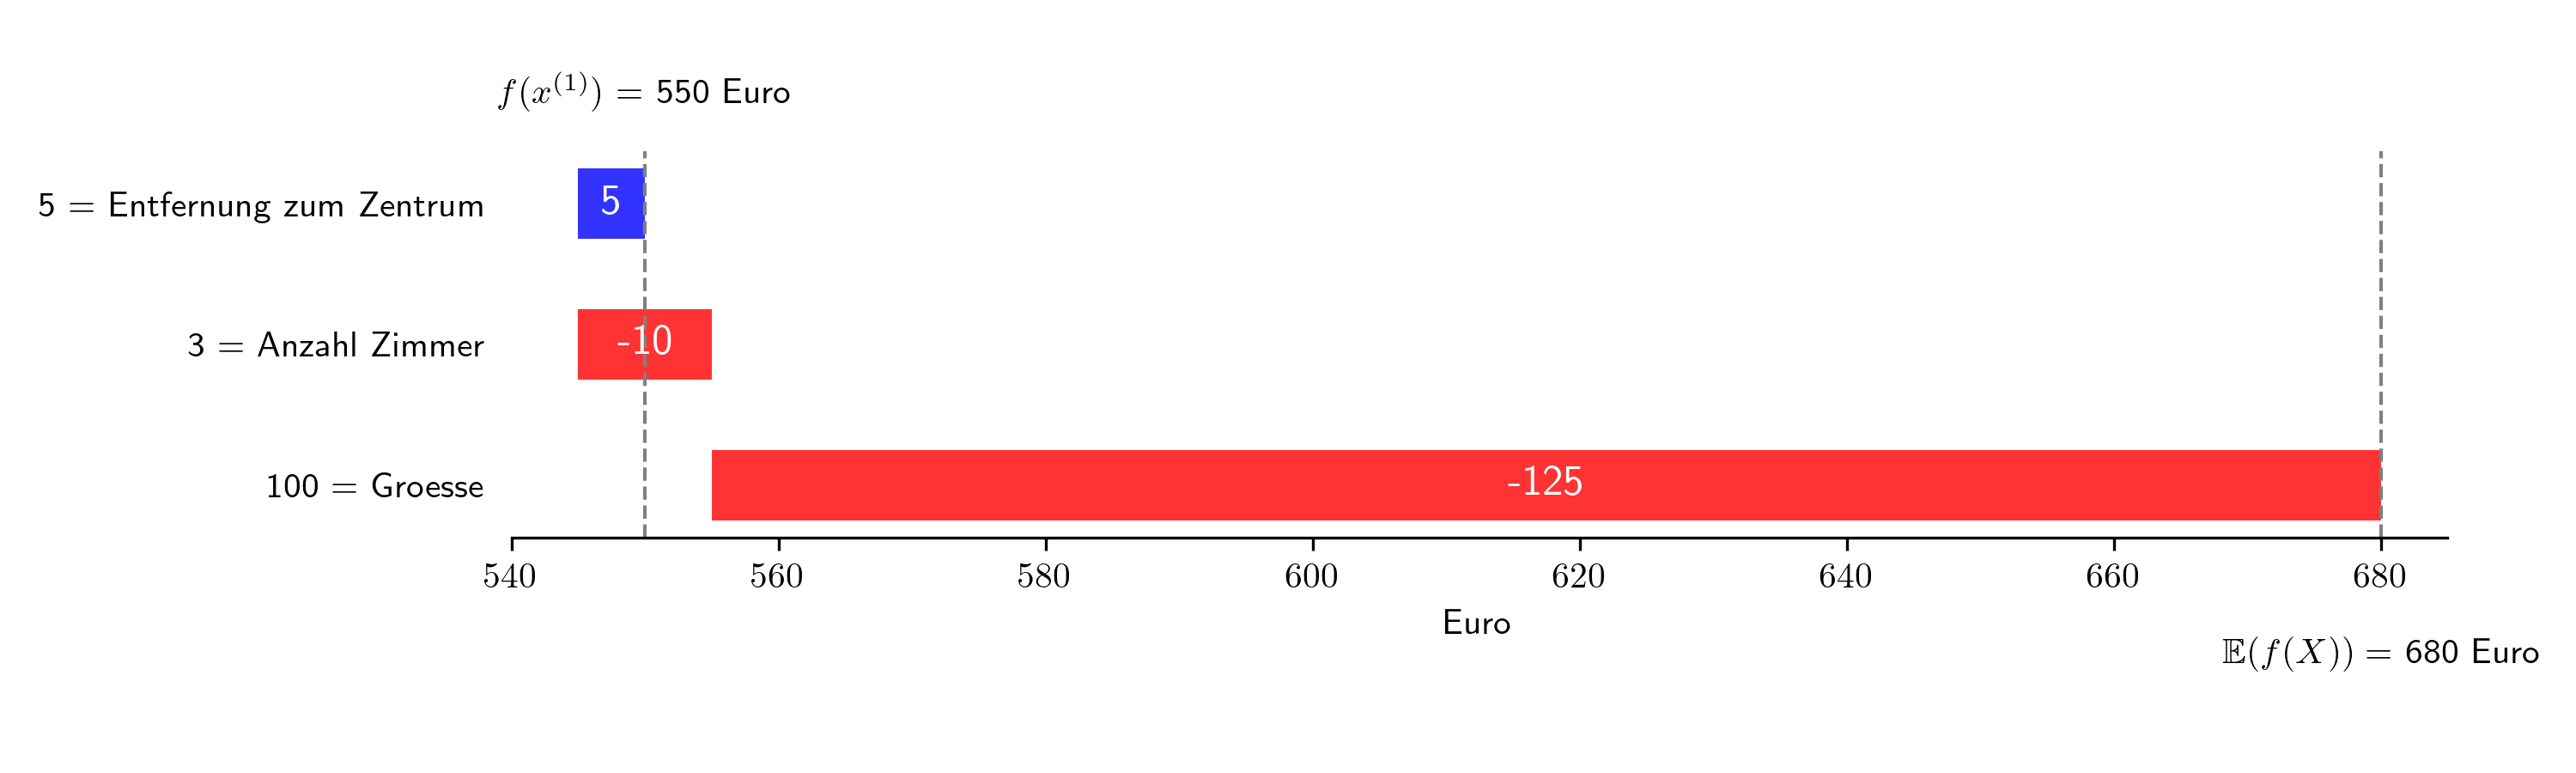
\includegraphics[width=1\textwidth]{../scripts/images/model-output-x1.png}
    Quelle: Eigene Darstellung, \ref{charts}.
    \label{pic:model-fx1}
\end{figure}

Das Modell $f(x^{(i)})$
prognostiziert im Mittel einen Immobilienpreis von 680 \euro{}. Im Vergleich zur
Verteilung des jeweiligen Merkmals, reduziert die Größe der 
Wohnung ($x_1^{(1)}$) und die Anzahl der Zimmer ($x_2^{(1)}$) die Prognose 
des Preises für die Immobilie $x^{(1)}$ um insgesamt 135 \euro{}, während die Entfernung zum Stadtzentrum
($x_3^{(1)}$) den Preis der Wohnung um 5 \euro{} erhöht, wie in Abbildung 
\ref{pic:model-fx1} veranschaulicht. Abbildung \ref{pic:model-fx2} visualisiert die SHAP-Werte für die Immobilie $x^{(2)}$:

\begin{figure}[!h]
    \caption{Beitrag der Merkmale $x_{j \in \{1, 2, 3\}}$ zur Modellvorhersage $f(x^{(2)})$.}
    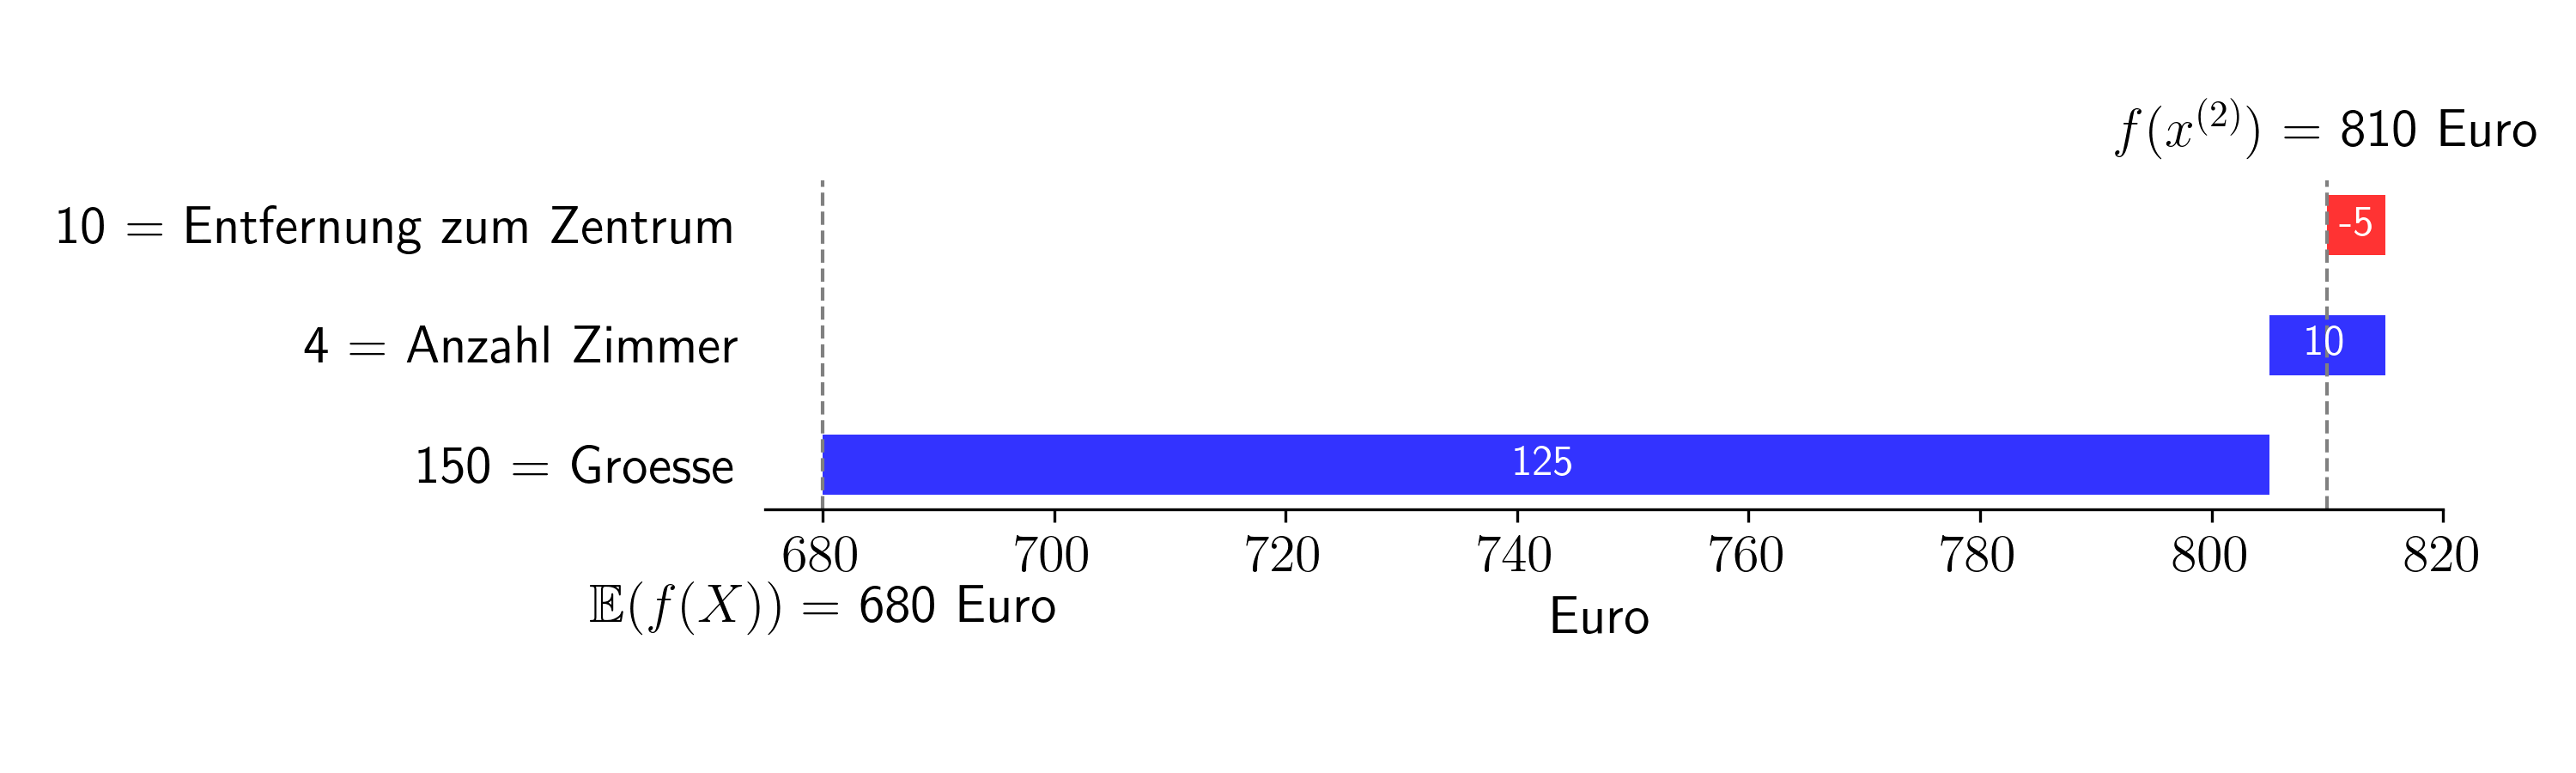
\includegraphics[width=1\textwidth]{../scripts/images/model-output-x2.png}
    Quelle: Eigene Darstellung, \ref{charts}.
    \label{pic:model-fx2}
\end{figure}


\section{Axiome}

Die in Tabellen \ref{tab:shapley_marginal_features_x1} und \ref{tab:shapley_marginal_features_x2} präsentierten Ergebnisse bieten eine Grundlage, 
um die Konformität der SHAP-Werte mit den etablierten Axiomen der Shapley-Werte, wie sie im 
Kapitel \ref{sec:axiome-shapley} diskutiert wurden, zu beurteilen. Die Axiome der SHAP-Werte stellen 
eine adaptierte und kontextualisierte Anwendung dieser Prinzipien auf die Interpretation von 
Modellvorhersagen dar \cite[S. 16f]{Algaba2019HandbookOT}.


\paragraph{Effizienz}

Das Effizienzaxiom besagt, dass die Summe der SHAP-Werte aller Merkmals für eine gegebene Beobachtung $x^{(i)}$ 
gleich der Differenz zwischen der Modellvorhersage für diese Beobachtung $f(x^{(i)})$ 
und der durchschnittlichen Modellvorhersage $\mathbb{E}(f(X))$ sein muss:

\begin{align}
    \sum_{j=1}^{p}\varphi_j^{(i)}(\mathcal{N}, f) = f(x^{(i)}) - \mathbb{E}(f(X)),
    \label{eq:eff}
\end{align}

\cite[S. 221]{Molnar_2022}. Für die Beobachtung $x^{(1)}$ aus Kapitel \ref{sec:example} und den Berechnungen 
für $f(x^{(1)})$ (Gleichung \ref{eq:fx1}), sowie $\mathbb{E}(f(X))$ (Gleichung \ref{eq:efx}) ergibt sich:

\begin{align}
    \sum_{j=1}^{3}\varphi_j^{(1)}(\mathcal{N}, f) &=  -130 \\ \notag
    f(x^{(1)}) - \mathbb{E}(f(X)) &= 550 - 680 = -130,   
\end{align}

womit das Effizienzaxiom erfüllt ist. Die Differenz der Vohersage 
einer konkreten Beobachtung zur durchschnittlichen 
Modellvorhersage wird auf alle Merkmale verteilt.

\paragraph{Symmetrie}

Das Symmetrieaxiom fordert, dass zwei Merkmale $i$ und $j$, die 
in jeder Koalition denselben Beitrag leisten, auch denselben SHAP-Wert 
erhalten müssen. In dem hier betrachteten Fall der Immobilienpreisprognose 
würde dies bedeuten, dass wenn zwei Merkmale, beispielsweise die Größe einer 
Wohnung und die Anzahl der Zimmer, immer den gleichen Einfluss auf den Preis hätten, 
unabhängig von der Kombination anderer Merkmale, ihre SHAP-Werte identisch 
sein müssen:

\begin{equation}
    v(\mathcal{S} \cup \{i\}) = v(\mathcal{S} \cup \{j\}), \; \forall\, \mathcal{S} \subseteq \mathcal{N} \setminus \{i, j\} \Rightarrow \varphi_i (\mathcal{N}, v) = \varphi_j (\mathcal{N}, v),
\end{equation}

\cite[S. 221]{Molnar_2022}. Dies wird durch die Tabellen \ref{tab:shapley_marginal_features_x1} und \ref{tab:shapley_marginal_features_x2} 
nicht illustriert, da jedes Merkmal einen unterschiedlichen Beitrag liefert, 
was die Anwendung dieses Axioms in diesem speziellen Fall ausschließt.

\paragraph{Null-Spieler-Eigenschaft (Dummy-Spieler-Eigenschaft)}

Ein Merkmal $i$, das keinen Einfluss auf die Modellvorhersage hat, erhält gemäß der 
Null-Spieler-Eigenschaft einen SHAP-Wert von Null. 
Im Kontext des Beispiels würde ein Merkmal, das keine Veränderung in der Vorhersage 
bewirkt, unabhängig von den anderen Merkmalen, einen SHAP-Wert von Null erhalten:

\begin{equation}
    v(\mathcal{S} \cup \{i\}) =  v(\mathcal{S}), \; \forall\, \mathcal{S} \subseteq \mathcal{N} \setminus \{i\} \Rightarrow \varphi_i (\mathcal{N}, v) = 0,
\end{equation}

\cite[S. 222]{Molnar_2022}. In der fiktiven Datenlage der Tabellen \ref{tab:shapley_marginal_features_x1} und \ref{tab:shapley_marginal_features_x2} hat jedes Merkmal 
einen gewissen Einfluss, sodass die Null-Spieler-Eigenschaft hier nicht beobachtet werden kann.

\paragraph{Additivität}

Das Additivitätsaxiom ist ein zentrales Konzept, das die Konsistenz von Shapley-Werten 
über die Zusammensetzung von Spielen hinweg beschreibt. Es garantiert, 
dass für zwei separate Spiele oder Modelle \(v\) und \(w\), die Summe der SHAP-Werte eines 
Merkmals über beide Spiele seinem SHAP-Wert im kombinierten Spiel entspricht:

\begin{equation}
    \varphi_i(\mathcal{N}, v + w) = \varphi_i (\mathcal{N}, v) + \varphi_i (\mathcal{N}, w).
\end{equation}

In Machine Learning-Modellen wie dem Random Forest, besonders bei Ensemble-Modellen, 
ist die Additivität relevant. Ein Random Forest besteht aus unabhängigen Entscheidungsbäumen, 
die zusammenarbeiten, um Vorhersagen zu treffen. Die SHAP-Werte der einzelnen Bäume 
können als additive Beiträge betrachtet werden, die den Gesamteinfluss eines Merkmals 
auf die Modellvorhersage zusammenfassen. \cite[S. 32]{Molnar_2023}.

\chapter{Komplexitätsbewältigung bei der Berechnung von SHAP-Werten}
\label{sec:estimators}

Die direkte Berechnung von SHAP-Werten kann bei Modellen mit einer 
großen Anzahl an Merkmalen rechnerisch anspruchsvoll sein. Im Kontext linearer Modelle, 
wie dem in dieser Arbeit verwendeten Immobilienpreis-Beispiel, 
ist die vollständige Ermittlung aller möglichen Kombinationen von Merkmalen und deren 
Beiträgen jedoch nicht notwendig. 

In einem linearen Modell sind die Beiträge der einzelnen Merkmale zur Vorhersage additiv 
und unabhängig voneinander. Dies ermöglicht eine direkte Ableitung der Beiträge 
jedes Merkmals aus den Modellkoeffizienten. Aufgrund dieser Eigenschaft 
liefert jedes Merkmal einen konstanten marginalen Beitrag, 
unabhängig von der Zusammensetzung der restlichen Koalition von Merkmalen. 
Theoretisch könnte daher für jedes Merkmal nur eine Koalition berechnet werden, 
um den SHAP-Wert zu bestimmen \cite[S. 38]{Molnar_2023}. Dies bestätigen die
Tabellen \ref{tab:shapley_marginal_features_x1} und \ref{tab:shapley_marginal_features_x2}
und die daraus ersichtlichen marginalen Beiträge, die über die jeweiligen Merkmale
unabhängig der ihnen beigetretenen Koalition konstant sind. So ist der marginale Beitrag für Merkmal $x_1^{(1)}$
zu allen möglichen Koalitionen stets $-125$.

Die Herausforderung bei der Berechnung von SHAP-Werten in realen Szenarien erwächst aus 
zwei zentralen Problembereichen: der Anzahl der Merkmale und der Notwendigkeit, 
über diese Merkmale zu integrieren. 

Die Anzahl möglicher Koalitionen von Merkmalen wächst exponentiell mit \( 2^p \) an, 
was bei einer großen Anzahl von Merkmalen \( p \) schnell zu einer nicht handhabbaren Berechnungskomplexität führt. 
Hinzu kommt die Schwierigkeit, dass für eine exakte Berechnung der SHAP-Werte eine Integration 
über die Merkmalsverteilungen erforderlich ist, was jedoch voraussetzt, dass die Verteilung der Merkmale bekannt ist. 
In der Praxis verfügt man meist nur über eine Stichprobe der Daten, ohne genaue Kenntnis der zugrundeliegenden Verteilungen \cite[S. 33]{Molnar_2023}.

Um diesen Herausforderungen zu begegnen, wird in diesem Kapitel die Anwendung von Monte Carlo Integration 
zur Schätzung von SHAP-Werten diskutiert. Diese Methoden ermöglichen es, durch Zufallsstichproben aus den vorhandenen Daten 
eine Approximation der Verteilungen zu erstellen und dadurch die notwendigen Integrationen näherungsweise auszuführen \cite[S. 34]{Molnar_2023}. 
Darüber hinaus werden Ansätze zur Stichprobenbildung von Koalitionen vorgestellt, die es erlauben, 
die rechnerische Last zu reduzieren, indem nicht alle Koalitionen betrachtet, sondern repräsentative Stichproben gezogen werden. 

\section{Approximation der marginalen Beiträge mittels Monte Carlo Integration}

Statt das Integral über eine unbekannte Verteilung zu berechnen, wie in Gleichung \ref{eq:shap-value-func},
nähert die Monte Carlo Integration dieses Integral durch den Durchschnitt einer großen Anzahl zufällig 
ausgewählter Beobachtungen aus dem Eingaberaum an \cite[S. 34]{Molnar_2023}. Die Monte Carlo Integration kann als ein erwartungstreuer Schätzer 
betrachtet werden, wenn die Anzahl der Zufallsstichproben $n$ hinreichend groß ist. Dies bedeutet, dass mit zunehmendem $n$ die Schätzung des Integrals 
immer genauer wird und gegen den wahren Wert des Integrals konvergiert. Dies basiert auf dem Gesetz der großen Zahlen, 
das besagt, dass der Durchschnitt einer großen Anzahl unabhängiger und identisch verteilter Zufallsvariablen gegen den Erwartungswert der Verteilung konvergiert \cite[S. 83]{Robert_Casella_2004}. 

Die Zufallsvariable $X_{C}^{(k)}$, die Merkmale die nicht in der Koalition $\mathcal{S}$ enthalten sind, 
entfällt und wird durch konkrete Beobachtungen $x_{C}^{(k)}$ aus der Datenbasis ersetzt, 
was eine wünschenswerte Vereinfachung darstellt. Das Integral $\int$ wird dadurch zur Summe $\sum$ und die Verteilung $\mathbb{P}$ wird durch eine große Anzahl zufällig 
ausgewählter Beobachtungen ersetzt und das Ergebnis anschließend über alle ausgewählten Beobachtungen $n$ gemittelt. 
$\hat{v}_{x^{(i)}, f}(\mathcal{S})$ ist somit ein Schätzer für den Wert der Koalition $\mathcal{S}$ und definiert als: 

\begin{align}
    \label{eq:monte-value}
    \hat{v}_{x^{(i)},f}(\mathcal{S}) = \frac{1}{n} \sum_{k=1}^{n} \Big(f(x^{(i)}_{\mathcal{S}} \cup x^{(k)}_{C}) - f(x^{(k)}) \Big)
\end{align}

Analog zu Gleichung \ref{eq:shap-marginal-func} ist dann zusammen mit Gleichung \ref{eq:monte-value} der marginale Beitrag 
$\hat{\Delta}_{\mathcal{S}, j}$ von Merkmal $j$ zur Koalition $\mathcal{S}$ gegeben als: 

\begin{align}
    \hat{\Delta}_{\mathcal{S}, j} &= \hat{v}_{x^{(i)},f}(\mathcal{S} \cup \{j\}) - \hat{v}_{x^{(i)},f}(\mathcal{S}) \\ \notag
        &= \frac{1}{n} \sum_{k=1}^{n} \Big(f(x^{(i)}_{\mathcal{S} \cup \{j\}} \cup x^{(k)}_{C \setminus \{j\}}) - f(x^{(i)}_{\mathcal{S}} \cup x^{(k)}_{C}) \Big)
\end{align}

und die SHAP-Werte $\hat{\varphi}_{j}^{(i)}$ über alle möglichen Koalitionen analog zu Gleichung \ref{eq:shap-eq}:

\begin{align}
    \label{eq:monte-shap-eq}
    \hat{\varphi}^{(i)}_{j} (\mathcal{N}, f) &= \sum_{\mathcal{S} \subseteq \mathcal{N} \setminus \{j\}} \frac{|\mathcal{S}|! \cdot (p - 1 - |\mathcal{S}|)!}{p!}\hat{\Delta}_{\mathcal{S}, j},
\end{align}

\cite[S.36]{Molnar_2023}.

\section{Schätzung von Koalitionen}

Obwohl die Monte Carlo Integration aus Gleichung \ref{eq:monte-shap-eq} eine praktische Methode zur Approximation der benötigten marginalen Beiträge in der 
SHAP-Wertberechnung bietet, bleibt die Herausforderung, alle möglichen Koalitionen der Merkmals zu evaluieren. 
Die Anzahl der Koalitionen wächst exponentiell mit der Anzahl der Merkmals. Daher sind Ansätze gefragt, die eine effiziente Schätzung der SHAP-Werte erlauben, 
ohne jede mögliche Koalition explizit zu berücksichtigen.

Insbesondere für lineare Modelle ohne Interaktionsterme wurde in Kpaitel \ref{sec:estimators} bereits gezeigt,
dass die Berechnung einer einzigen Koalition für jedes Merkmal ausreichend ist \cite[S. 38]{Molnar_2023}.
In einem solchen Modell wird angenommen, dass die Beziehung zwischen den unabhängigen 
Variablen und der abhängigen Variable additiv ist, das heißt, es gibt keine Terme im Modell, 
die das Produkt von zwei oder mehr unabhängigen Variablen enthalten, um mögliche Interaktionseffekte 
zwischen ihnen zu repräsentieren.

Neben dem Linearen SHAP Estimator in Kapitel \ref{subsec:linear-shap-estimator} wird die Schätzung durch Permutationen in Kapitel 
\ref{subsec:permutation} diskutirert. Anstelle der Iteration über alle Koallitionen, werden repräsentative Stichproben zur Berechnung
herangezogen. 

Beide Verfahren bieten Strategien zur Reduzierung der Berechnungskomplexität, 
indem sie Annahmen über die Eigenschaften des Modells und der Daten treffen. 
Weitere Ansätze werden in Kapitel \ref{sec:shap-package} angesprochen.


\subsection{Linearer SHAP Estimator für lineare Modelle}
\label{subsec:linear-shap-estimator}

Für lineare Modelle bietet der lineare SHAP Estimator eine direkte und effiziente 
Methode zur Berechnung der SHAP-Werte. Diese Methode beruht auf der Annahme 
der Unabhängigkeit der Eingabemerkmale. Unter dieser Voraussetzung können 
die SHAP-Werte direkt aus den Gewichtungskoeffizienten des linearen Modells 
abgeleitet werden.

Ein lineares Modell wird typischerweise in der Form 
\( f(x) = \sum_{j=1}^{p} \beta_j x_j + b \) ausgedrückt, wobei \( \beta_j \) der 
Gewichtungskoeffizient für das Merkmal \( j \) ist und \( b \) den 
Achsenabschnitt (Bias) darstellt. Der lineare SHAP Estimator nutzt 
diese Koeffizienten, um die Beiträge jedes Merkmals zur Modellvorhersage 
zu bestimmen. Der SHAP-Wert für ein Merkmal \( j \) wird dann definiert als:

\begin{align}
    \varphi_j^{(i)}(f, x) = \beta_j (x_j^{(i)} - \mathbb{E}[X_j]),
\end{align}

wobei \( \mathbb{E}[X_j] \) der Erwartungswert des Merkmals \( j \) über den 
Datensatz ist. Der SHAP-Wert für den Achsenabschnitt (Bias) ist gleich 
dem Achsenabschnitt des Modells: \( \varphi_0(f, x) = b \) \cite[S. 6]{NIPS2017_8a20a862}.

Aufgrund der Unabhängigkeit der Eingabemerkmale, kann das arithmetische Mittel aus Kapitel 
\ref{sec:example} Gleichung \ref{eq:e} als erwartungstreuer Schätzer für den Erwartungswert verwendet werden:

\begin{align}
    \varphi_j^{(i)}(f, x) = \beta_j \Big(x_j^{(i)} - \frac{1}{n} \sum_{k=1}^{n} (x_j^{(k)})\Big),
\end{align}

Das Effizienzaxiom aus Gleichung \ref{eq:eff} is erfüllt:

\begin{align}
    \sum_{j=1}^p \varphi_j^{(i)}(f, x) &= \sum_{j=1}^p  \Big( \beta_j x_j^{(i)} - \mathbb{E}[\beta_j X_j]\Big) \\ \notag
                                    &= \beta_0 + \sum_{j=1}^p \beta_j x_j^{(i)} - ( \beta_0 + \sum_{j=1}^p \mathbb{E}[\beta_j X_j]) \\ \notag
                                    &= f(x) - \mathbb{E}[f(X)],
\end{align}                 

\cite[S. 48]{Molnar_2023}.

Diese Berechnung der SHAP-Werte basiert auf der Idee, dass die Änderung 
des Modelloutputs, die durch das Abweichen eines Merkmals von seinem 
Erwartungswert entsteht, direkt durch den entsprechenden Gewichtungskoeffizienten 
des linearen Modells beschrieben werden kann. Dieser Ansatz ermöglicht eine 
schnelle und genaue Berechnung der SHAP-Werte für lineare Modelle und ist 
besonders nützlich, um die Auswirkungen einzelner Merkmals in einem solchen 
Modell zu interpretieren. 

\subsection{Schätzung durch Permutationen}
\label{subsec:permutation}

Der Einsatz von Permutationen zur Schätzung von SHAP-Werten bietet eine 
praktikable Alternative zur vollständigen Auswertung aller Merkmalskoalitionen. 
Dieses Verfahren ist insbesondere in Szenarien mit einer hohen Anzahl von Merkmalen von Vorteil, 
da es die Berechnungslast reduziert, ohne die Genauigkeit der Schätzung wesentlich zu beeinträchtigen. 
Im Folgenden wird die Methode anhand eines Beispiels illustriert und die Anwendung im Kontext des in 
Kapitel \ref{sec:example} eingeführten linearen Modells beschrieben.

In einem ersten Schritt wird eine zufällige $k$-te Permutation der Merkmale $o(k)$ gewählt.
Beispielsweise könnte $o(k) = (x_2, x_3, x_1)$ eine solche Permutation darstellen.
Wird das Merkmal $j$, für das der SHAP-Wert berechnet werden soll, als das dritte Merkmal $j=3$ angenommen, 
ergibt sich der marginale Beitrag $\hat{\Delta}_{o(k), j}$ analog zu Gleichung \ref{eq:monte-shap-eq} aus der Differenz
der Koalitionen mit und ohne dem betrachteten Merkmal:

\begin{align}
    \label{eq:permu-shap-eq}
    \hat{\varphi}^{(i)}_{j} (\mathcal{N}, f) &= \frac{1}{m}\sum_{k=1}^{m}\hat{\Delta}_{o(k), j},
\end{align}

Dieser Prozess wird für eine Anzahl von $m$ Permutationen durchgeführt. Die Wahl von $m$,
die kleiner als die Gesamtzahl der Merkmale sein kann, hängt von der gewünschten Approximationsgenauigkeit
ab. Eine größere Anzahl von Permutationen $m$ führt zu einer präziseren Annäherung an den tatsächlichen SHAP-Wert.

Die geschätzten marginalen Beiträge $\hat{\Delta}_{o(k), j}$ werden dann über die $m$ Permutationen gemittelt:

\begin{align}
\hat{\varphi}^{(i)}{j} (\mathcal{N}, f) &= \frac{1}{m}\sum{k=1}^{m}\hat{\Delta}_{o(k), j},
\end{align}

Durch diese Methodik wird der Berechnungsaufwand bei der Ermittlung von SHAP-Werten 
signifikant verringert, was besonders bei Modellen mit einer großen Anzahl von Merkmalen von 
Bedeutung ist. Der hier vorgestellte Ansatz ermöglicht es, mit einer begrenzten Anzahl von 
Permutationen eine aussagekräftige Schätzung der SHAP-Werte zu erhalten \cite[S. 39]{Molnar_2023}.

Zusätzlich zur Mittelung der geschätzten marginalen Beiträge bietet die Methode der Permutationen 
die Möglichkeit, die Effekte von Vorwärts- und Rückwärtspropagation zu untersuchen, 
indem die Reihenfolge der Merkmale sowohl in ihrer ursprünglichen als auch in umgekehrter 
Abfolge betrachtet wird. Für eine detaillierte Darstellung dieser Technik und ihrer 
Auswirkungen auf die SHAP-Wertberechnung sei auf die weiterführende Literatur verwiesen \cite[S. 39f]{Molnar_2023}.



\chapter{Praktische Anwendung von SHAP auf lineare Modelle}

In diesem Kapitel wird der Einsatz des SHAP-Frameworks zur Interpretation linearer Modelle im 
Kontext des maschinellen Lernens untersucht. Lineare Modelle, gekennzeichnet durch ihre Transparenz 
und einfache Struktur, bilden oft die Basis für das Verständnis komplexerer Algorithmen. 
Dennoch bleibt die Herausforderung bestehen, die Beiträge individueller Merkmale zur Modellvorhersage zu 
quantifizieren und zu interpretieren.

Die Anwendung von SHAP-Werten ermöglicht es, diesen Herausforderungen zu begegnen und Einblicke in 
die Modellvorhersagen zu gewähren, die über traditionelle Methoden hinausgehen. 
Dieses Kapitel führt in die Grundlagen des \textsf{shap}-Pakets ein, demonstriert dessen Anwendung auf einen 
spezifischen Datensatz und diskutiert die Berechnung sowie Interpretation der resultierenden SHAP-Werte.

\section{Lineare Modelle als analytische Grundlage}

In linearen Regressionsmodellen wird die Zielgröße als eine gewichtete Kombination der Eingangsmerkmale bestimmt. 
Die einfache lineare Struktur dieser Modelle erleichtert das Verständnis der Beziehungen zwischen den Eingangsdaten 
und den Vorhersagen. 

Lineare Modelle sind ein grundlegendes Werkzeug in der statistischen Modellierung und dienen dazu, das Verhältnis zwischen 
einer abhängigen Variablen, die üblicherweise mit $y^{(i)}$ bezeichnet wird, 
und einem oder mehreren Prädiktoren, den unabhängigen Variablen $x_i$, zu erfassen. 
Diese Beziehungen werden mittels linearer Gleichungen dargestellt, die für jede 
einzelne Beobachtung $i$ im Datensatz folgendermaßen formuliert werden können:

\begin{equation}
    y^{(i)} = \beta_0 + \sum_{j=1}^{p} \beta_j x^{(i)}_j + \epsilon^{(i)},
\label{eq:reg-model}
\end{equation}

wobei das Ergebnis, das von einem linearen Modell für eine gegebene Beobachtung vorhergesagt wird, sich als Summe der mit 
Gewichten $\beta_j$ versehenen Merkmale $p$ ergibt.

Hierbei stellt $y^{(i)}$ den beobachteten Wert der abhängigen Variablen für die Beobachtungseinheit
$i$ dar. Der Term $\beta_0$ ist der Achsenabschnitt oder y-Achsenabschnitt des Modells, 
welcher den erwarteten Wert von $y$ darstellt, wenn alle unabhängigen Variablen $x$ null sind. 
Die Summe $\sum_{j=1}^{p} \beta_j x^{(i)}_j$ berechnet sich aus den Produkten der Koeffizienten 
$\beta_j$ und den Werten der unabhängigen Variablen $x^{(i)}_j$ für jede Beobachtungseinheit $i$ 
und jeden Prädiktor $j$, wobei die Koeffizienten $\beta_j$ den geschätzten Einfluss der 
entsprechenden unabhängigen Variablen auf die abhängige Variable beschreiben.

Der Fehlerterm $\epsilon^{(i)}$ steht für die Residuen, also die Differenzen zwischen den beobachteten 
und durch das Modell geschätzten Werten von $y^{(i)}$. Es wird angenommen, dass diese Fehler normalverteilt sind, 
was bedeutet, dass Abweichungen in beiden Richtungen um den Mittelwert (hier Null) 
mit abnehmender Wahrscheinlichkeit für größere Fehler auftreten \cite[S. 37]{Molnar_2022}.

In einem linearen Modell stellt der Achsenabschnitt die Basislinie dar, an der die Auswirkungen aller 
anderen Merkmale gemessen werden. Dieser Wert gibt an, was das Modell für die Zielvariable vorhersagen 
würde, wenn alle anderen Merkmale nicht vorhanden wären – der Ausgangspunkt der Vorhersage 
für einen Datensatz, in dem alle anderen Variablen auf null gesetzt sind. 
Es ist wichtig zu erwähnen, dass der Achsenabschnitt für sich genommen nicht immer eine praktische 
Bedeutung hat, da es selten vorkommt, dass alle Variablen tatsächlich den Wert null annehmen. 
Die wahre Aussagekraft des Achsenabschnitts tritt zutage, wenn die Daten so standardisiert wurden, 
dass ihre Mittelwerte bei null und die Standardabweichung bei eins liegen. Unter diesen Umständen repräsentiert der Achsenabschnitt 
die erwartete Zielvariable für einen hypothetischen Fall, in dem alle Merkmale ihren Durchschnittswert 
aufweisen.

Bei der Betrachtung einzelner Merkmale innerhalb des Modells sagt das Gewicht $\beta_j$ eines Merkmals, 
um wie viel sich die Zielvariable $y^{(i)}$ ändert, wenn das Merkmal $x^{(i)}_j$ um eine Einheit erhöht wird – und zwar unter 
der Annahme, dass alle anderen Merkmale unverändert bleiben. 
Dies ermöglicht es, den isolierten Effekt eines jeden Merkmals auf die Vorhersage zu verstehen \cite[S. 39]{Molnar_2022}.

Die optimalen Gewichte, oder Koeffizienten, eines linearen Regressionsmodells werden üblicherweise durch ein Verfahren bestimmt, 
das als Methode der kleinsten Quadrate (engl. \textit{Ordinary Least Squares}, OLS) bekannt ist. 
Diese Methode sucht die Koeffizienten \( \beta_0, \ldots, \beta_p \), welche die Summe der quadrierten 
Differenzen zwischen den beobachteten Werten der Zielvariablen \( y^{(i)} \) und den von dem Modell 
vorhergesagten Werten minimieren:

\begin{equation}
    \hat{\beta} = \arg \underset{\beta_0, \ldots, \beta_p}{\min} \ \sum_{i=1}^{n} \left( y^{(i)} - \left( \beta_0 + \sum_{j=1}^{p} \beta_j x_j^{(i)}\right)\right)^2.
\end{equation}

Das Ergebnis der Minimierung, \( \hat{\beta} \) stellt den Vektor der geschätzten Koeffizienten dar \cite[S. 37]{Molnar_2022}. 
In der vorliegenden Arbeit wird das Python-Paket \textsf{scikit-learn}\footnote{\url{https://scikit-learn.org}} verwendet, um die lineare Regression durchzuführen und die Koeffizienten 
\( \hat{\beta} \) zu bestimmen. 


\section{Einführung in das \textsf{shap} Python-Paket}
\label{sec:shap-package}

Das Python-Paket \textsf{shap}\footnote{\url{https://shap.readthedocs.io}} ist eine Open-Source-Bibliothek, die es Nutzern ermöglicht, 
die Auswirkungen von Merkmalen auf Vorhersagen von maschinellen Lernmodellen zu interpretieren und zu visualisieren. 
Entwickelt wurde die Bibliothek ursprünglich von Scott Lundberg und weiteren Mitwirkenden im Rahmen der Forschungsarbeit 
an der University of Washington \cite{NIPS2017_8a20a862}. Das Paket basiert auf dem Konzept der Shapley-Werte aus der kooperativen Spieltheorie 
und überträgt diese auf den Kontext des maschinellen Lernens, um als Tool für die Interpretierbarkeit und Erklärbarkeit 
von Modellvorhersagen zu dienen.

\urldef{\ploturl}\url{https://shap.readthedocs.io/en/latest/api.html#plots}

Die Kernfunktion des \textsf{shap}-Pakets ist die Berechnung von SHAP-Werten, welche die Auswirkung der 
Einzelmerkmale auf die Modellvorhersage quantifizieren. Jeder SHAP-Wert ist ein Maß dafür, wie viel jedes Merkmal 
zur Vorhersage beigetragen hat, im Vergleich zu einer durchschnittlichen Vorhersage über den gesamten Datensatz. 
Diese Werte sind besonders wertvoll, weil sie ein Maß für die Bedeutung jedes Merkmals liefern, 
das sowohl lokal (für einzelne Vorhersagen) als auch global (über das gesamte Modell) interpretiert werden kann.

Mit \textsf{shap} können Benutzer die Vorhersagen einer Vielzahl von Modellen interpretieren, 
von linearen Modellen bis hin zu komplexen Konstrukten wie tiefe neuronale Netzwerke. 
Die Bibliothek bietet eine vielseitige Auswahl an Visualisierungsoptionen, darunter Beeswarm-Plots, Dependence-Plots und 
Bar-Plots, die es ermöglichen, die SHAP-Werte intuitiv zu verstehen. Eine Übersicht aller Visualisierungsoptionen ist in der Dokumentation 
des Pakets zu finden\footnote{\ploturl}.
Diese Visualisierungen erleichtern es, Muster und Beiträge einzelner Merkmale zu erkennen, 
was nicht nur wertvolle Einblicke in die Leistung des Modells bietet, sondern auch zu faireren und transparenteren 
Modellentscheidungen führen kann. 

\urldef{\shapurl}\url{https://shap.readthedocs.io/en/latest/api.html#explainers}
\urldef{\exacturl}\url{https://github.com/shap/shap/blob/master/shap/explainers/_exact.py}

Im Kapitel \ref{subsec:linear-shap-estimator} wurde bereits der LinearExplainer aus dem \textsf{shap}-Paket 
vorgestellt, ein Beispiel für die verschiedenen Estimators, die das Paket in Form von Explainern bereitstellt. 
Das Paket bietet eine Vielzahl von Explainern, die auf unterschiedliche Modelltypen zugeschnitten sind. 
Einer der bemerkenswerten Aspekte von \textsf{shap} ist der auto Modus des Estimators, 
der automatisch den am besten geeigneten Explainer für das gegebene Modell auswählt. 
Diese Funktion ist besonders nützlich, da sie die Komplexität der Auswahl des richtigen Explainers 
reduziert und den Anwendungsprozess vereinfacht. Speziell für Modelle mit ca. 15 Merkmalen\footnote{\exacturl} wählt der 
auto Modus den exakten Explainer, der präzise SHAP-Werte auf Grundlage aller Daten und Koalitionen berechnet, was für Modelle mit einer geringeren Anzahl 
von Merkmalen effizient und praktikabel ist \cite[S. 40f]{Molnar_2023}. Eine Übersicht der zur Verfügung stehenden \textsf{shap}-Explainern ist in der
Dokumentation des Pakets zu finden\footnote{\shapurl}. 


\section{Einführung in den Datensatz}


Der Concrete Compressive Strength Datensatz ist eine umfassende Sammlung von Daten, 
die die Druckfestigkeit von Beton in Bezug auf verschiedene Bestandteile und das Alter des Betons untersucht. 
Die Bestandteile umfassen Zement, Hochofenschlacke, Flugasche, Wasser, Superplastifikator, 
groben Zuschlag und feinen Zuschlag \cite{misc_concrete_compressive_strength_165}.

\textbf{Ziel der Regression:} Das Ziel ist es, die Druckfestigkeit von Beton in Megapascal basierend 
auf seiner Zusammensetzung und dem Alter vorherzusagen. Diese Vorhersage ist entscheidend, 
da Beton das Fundament der modernen Welt bildet und seine Festigkeit für die Sicherheit und 
Langlebigkeit von Bauwerken von größter Bedeutung ist.

Der Datensatz umfasst folgende Variablen:

\begin{itemize}
    \item \textbf{\texttt{cement} (Zement)}: Menge an Zement (kg in einem m³ Gemisch). Zement ist ein Hauptbestandteil von Beton und wesentlich für dessen Festigkeit.
    \item \textbf{\texttt{blast} (Hochofenschlacke)}: Menge an Hochofenschlacke (kg in einem m³ Gemisch). Schlacke kann die Festigkeit und Haltbarkeit von Beton verbessern.
    \item \textbf{\texttt{ash} (Flugasche)}: Menge an Flugasche (kg in einem m³ Gemisch). Flugasche wird als Ersatz für Zement verwendet und beeinflusst die Verarbeitbarkeit und Festigkeit.
    \item \textbf{\texttt{water} (Wasser)}: Menge an Wasser (kg in einem m³ Gemisch). Wasser ist für die Hydratation des Zements und die Konsistenz des Betons notwendig.
    \item \textbf{\texttt{superplasticizer} (Superplastifikator)}: Menge an Superplastifikator (kg in einem m³ Gemisch). Superplastifikatoren verbessern die Fließfähigkeit und Verarbeitbarkeit von Beton.
    \item \textbf{\texttt{coarse} (Grober Zuschlag)}: Menge an grobem Zuschlag (kg in einem m³ Gemisch). Grober Zuschlag trägt zur Stabilität und Struktur des Betons bei.
    \item \textbf{\texttt{fine} (Feiner Zuschlag)}: Menge an feinem Zuschlag (kg in einem m³ Gemisch). Feiner Zuschlag beeinflusst die Dichte und die Oberflächeneigenschaften des Betons.
    \item \textbf{\texttt{age} (Alter)}: Alter des Betons in Tagen. Das Alter hat einen signifikanten Einfluss auf die Festigkeit des Betons.
    \item \textbf{\texttt{strength} (Druckfestigkeit)}: Die tatsächliche Druckfestigkeit von Beton (MPa). Dies ist die Zielvariable, die modelliert wird.
\end{itemize}
 
Die Bedeutung dieses Themas liegt in der zentralen Rolle, die Beton im Bauwesen spielt. 
Als eines der am meisten verwendeten Materialien weltweit, ist die genaue Vorhersage seiner Festigkeit von entscheidender 
Bedeutung für die Planung und den Bau sicherer und langlebiger Strukturen. Dieser Datensatz bietet daher wertvolle Einblicke für Ingenieure und Forscher, 
um die Eigenschaften und das Verhalten von Beton besser zu verstehen und zu optimieren.

\section{Explorative Datenanalyse \& Datenaufbereitung}

Der Datensatz wurde in Python mithilfe der Bibliothek \textsf{pandas} als \textsf{Dataframe} eingelesen.
Der vollständige Quellcode für das Einlesen der Daten sowie alle weiteren Analyseschritte ist 
im Anhang \ref{linreg} dieser Arbeit zu finden.

Tabelle \ref{tab:df-head} zeigt die ersten fünf Beobachtungen des Datensatzes:

\begin{table}[!h]
    \caption{Auszug aus dem Concrete Compressive Strength Datensatz.}
    \footnotesize
    \begin{tabularx}{\textwidth}{Xrrrrrrrrr}
    \toprule
    Index & \rotatebox{90}{cement} & \rotatebox{90}{blast} & \rotatebox{90}{ash} & \rotatebox{90}{water} & \rotatebox{90}{superplasticizer} & \rotatebox{90}{coarse} & \rotatebox{90}{fine} & \rotatebox{90}{age} & \rotatebox{90}{strength} \\
    \midrule
    0 & 540.0 & 0.0 & 0.0 & 162.0 & 2.5 & 1040.0 & 676.0 & 28 & 79.986111 \\
    1 & 540.0 & 0.0 & 0.0 & 162.0 & 2.5 & 1055.0 & 676.0 & 28 & 61.887366 \\
    2 & 332.5 & 142.5 & 0.0 & 228.0 & 0.0 & 932.0 & 594.0 & 270 & 40.269535 \\
    3 & 332.5 & 142.5 & 0.0 & 228.0 & 0.0 & 932.0 & 594.0 & 365 & 41.052780 \\
    4 & 198.6 & 132.4 & 0.0 & 192.0 & 0.0 & 978.4 & 825.5 & 360 & 44.296075 \\
    \bottomrule
    \end{tabularx}
    \label{tab:df-head}
    \normalsize\\
    Quelle: Eigene Darstellung, \ref{linreg}.
\end{table}

\begin{table}[!h]
    \caption{Statistische Übersicht des Concrete Compressive Strength Datensatzes.}
    \footnotesize
    \begin{tabularx}{\textwidth}{Xrrrrrrr}
    \toprule
    Variable & mean & std & min & 25\% & 50\% & 75\% & max \\
    \midrule
    cement & 278.629 & 104.345 & 102.0 & 190.68 & 265.0 & 349.0 & 540.0 \\
    blast & 72.043 & 86.171 & 0.0 & 0.0 & 20.0 & 142.5 & 359.4 \\
    ash & 55.535 & 64.207 & 0.0 & 0.0 & 0.0 & 118.27 & 200.1 \\
    water & 182.074 & 21.341 & 121.75 & 166.61 & 185.7 & 192.94 & 247.0 \\
    superplasticizer & 6.032 & 5.92 & 0.0 & 0.0 & 6.1 & 10.0 & 32.2 \\
    coarse & 974.376 & 77.58 & 801.0 & 932.0 & 968.0 & 1031.0 & 1145.0 \\
    fine & 772.687 & 80.34 & 594.0 & 724.3 & 780.0 & 822.2 & 992.6 \\
    age & 45.857 & 63.735 & 1.0 & 7.0 & 28.0 & 56.0 & 365.0 \\
    strength & 35.250 & 16.285 & 2.332 & 23.524 & 33.798 & 44.868 & 82.599 \\
    \bottomrule
    \end{tabularx}
    \label{tab:statistics}
    \normalsize
    \\ Quelle: Eigene Darstellung, \ref{linreg}.
\end{table}

Tabelle \ref{tab:statistics} offenbart eine signifikante Variabilität und Bandbreite 
in den Werten aller Variablen. Um eine gleichmäßigere Verteilung für die Regressionsanalyse 
zu erzielen und den Einfluss von Ausreißern zu reduzieren, wurde eine logarithmische Transformation 
auf die Daten angewendet. Abbildung \ref{pic:box} zeigt das Minimum, das untere Quartil, den Median, das obere Quartil und das Maximum
der jeweiligen Merkmale vor und nach der logarthimischen Transformation. 


\begin{figure}[!h]
    \caption{Boxplot der Merkmale vor und nach der Log-Transformation.}
    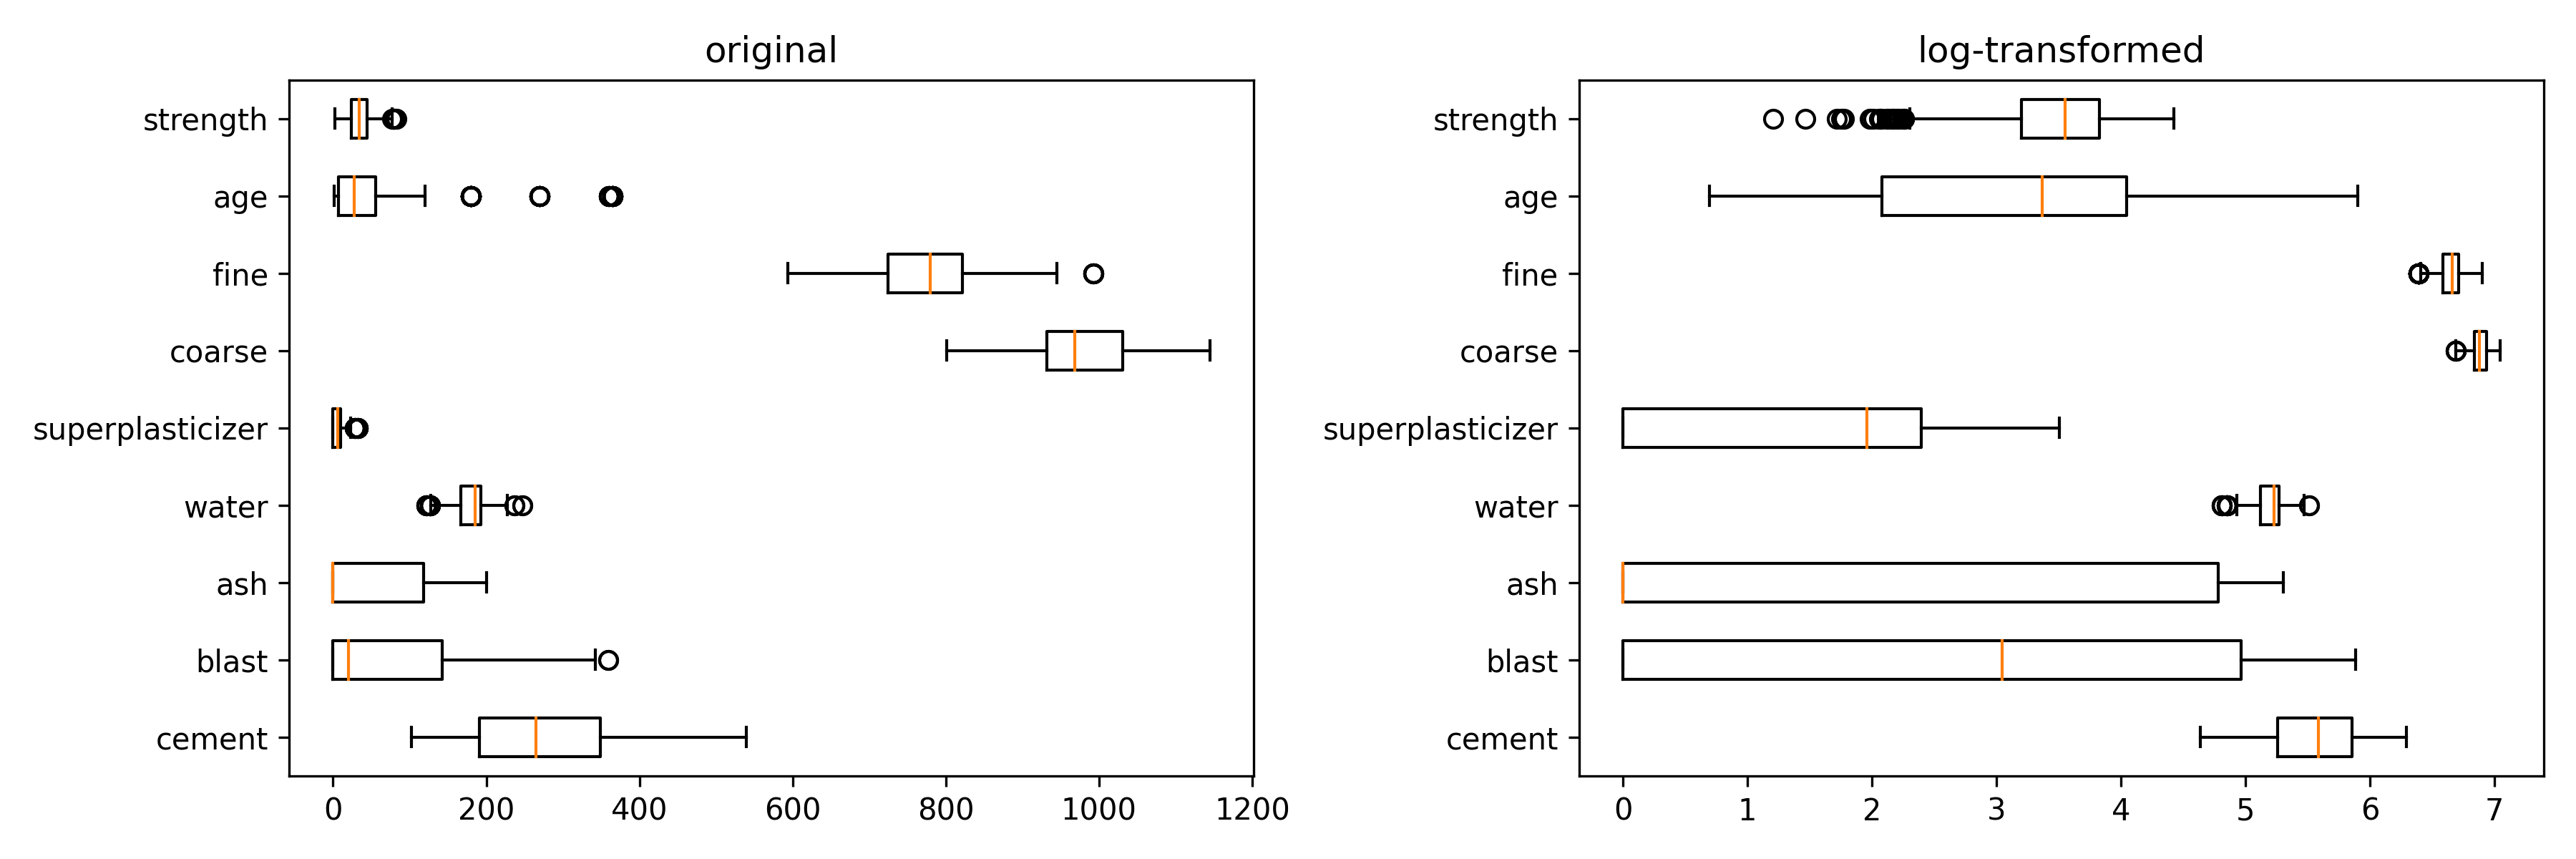
\includegraphics[width=1\textwidth]{../scripts/images/boxplot.png}
    Quelle: Eigene Darstellung, \ref{linreg}.
    \label{pic:box}
\end{figure}

Diese Transformation hilft, die Skalierung der Variablen zu vereinheitlichen 
und die Datenverteilung zu normalisieren, was für die Effektivität des Regressionsmodells vorteilhaft ist.

Abbildung \ref{pic:hist} zeigt die Häufigkeitsverteilung aller Merkmale des Datensatzes nach der logarithmischen Transformation. 

\begin{figure}[!h]
    \caption{Verteilungen der Merkmale.}
    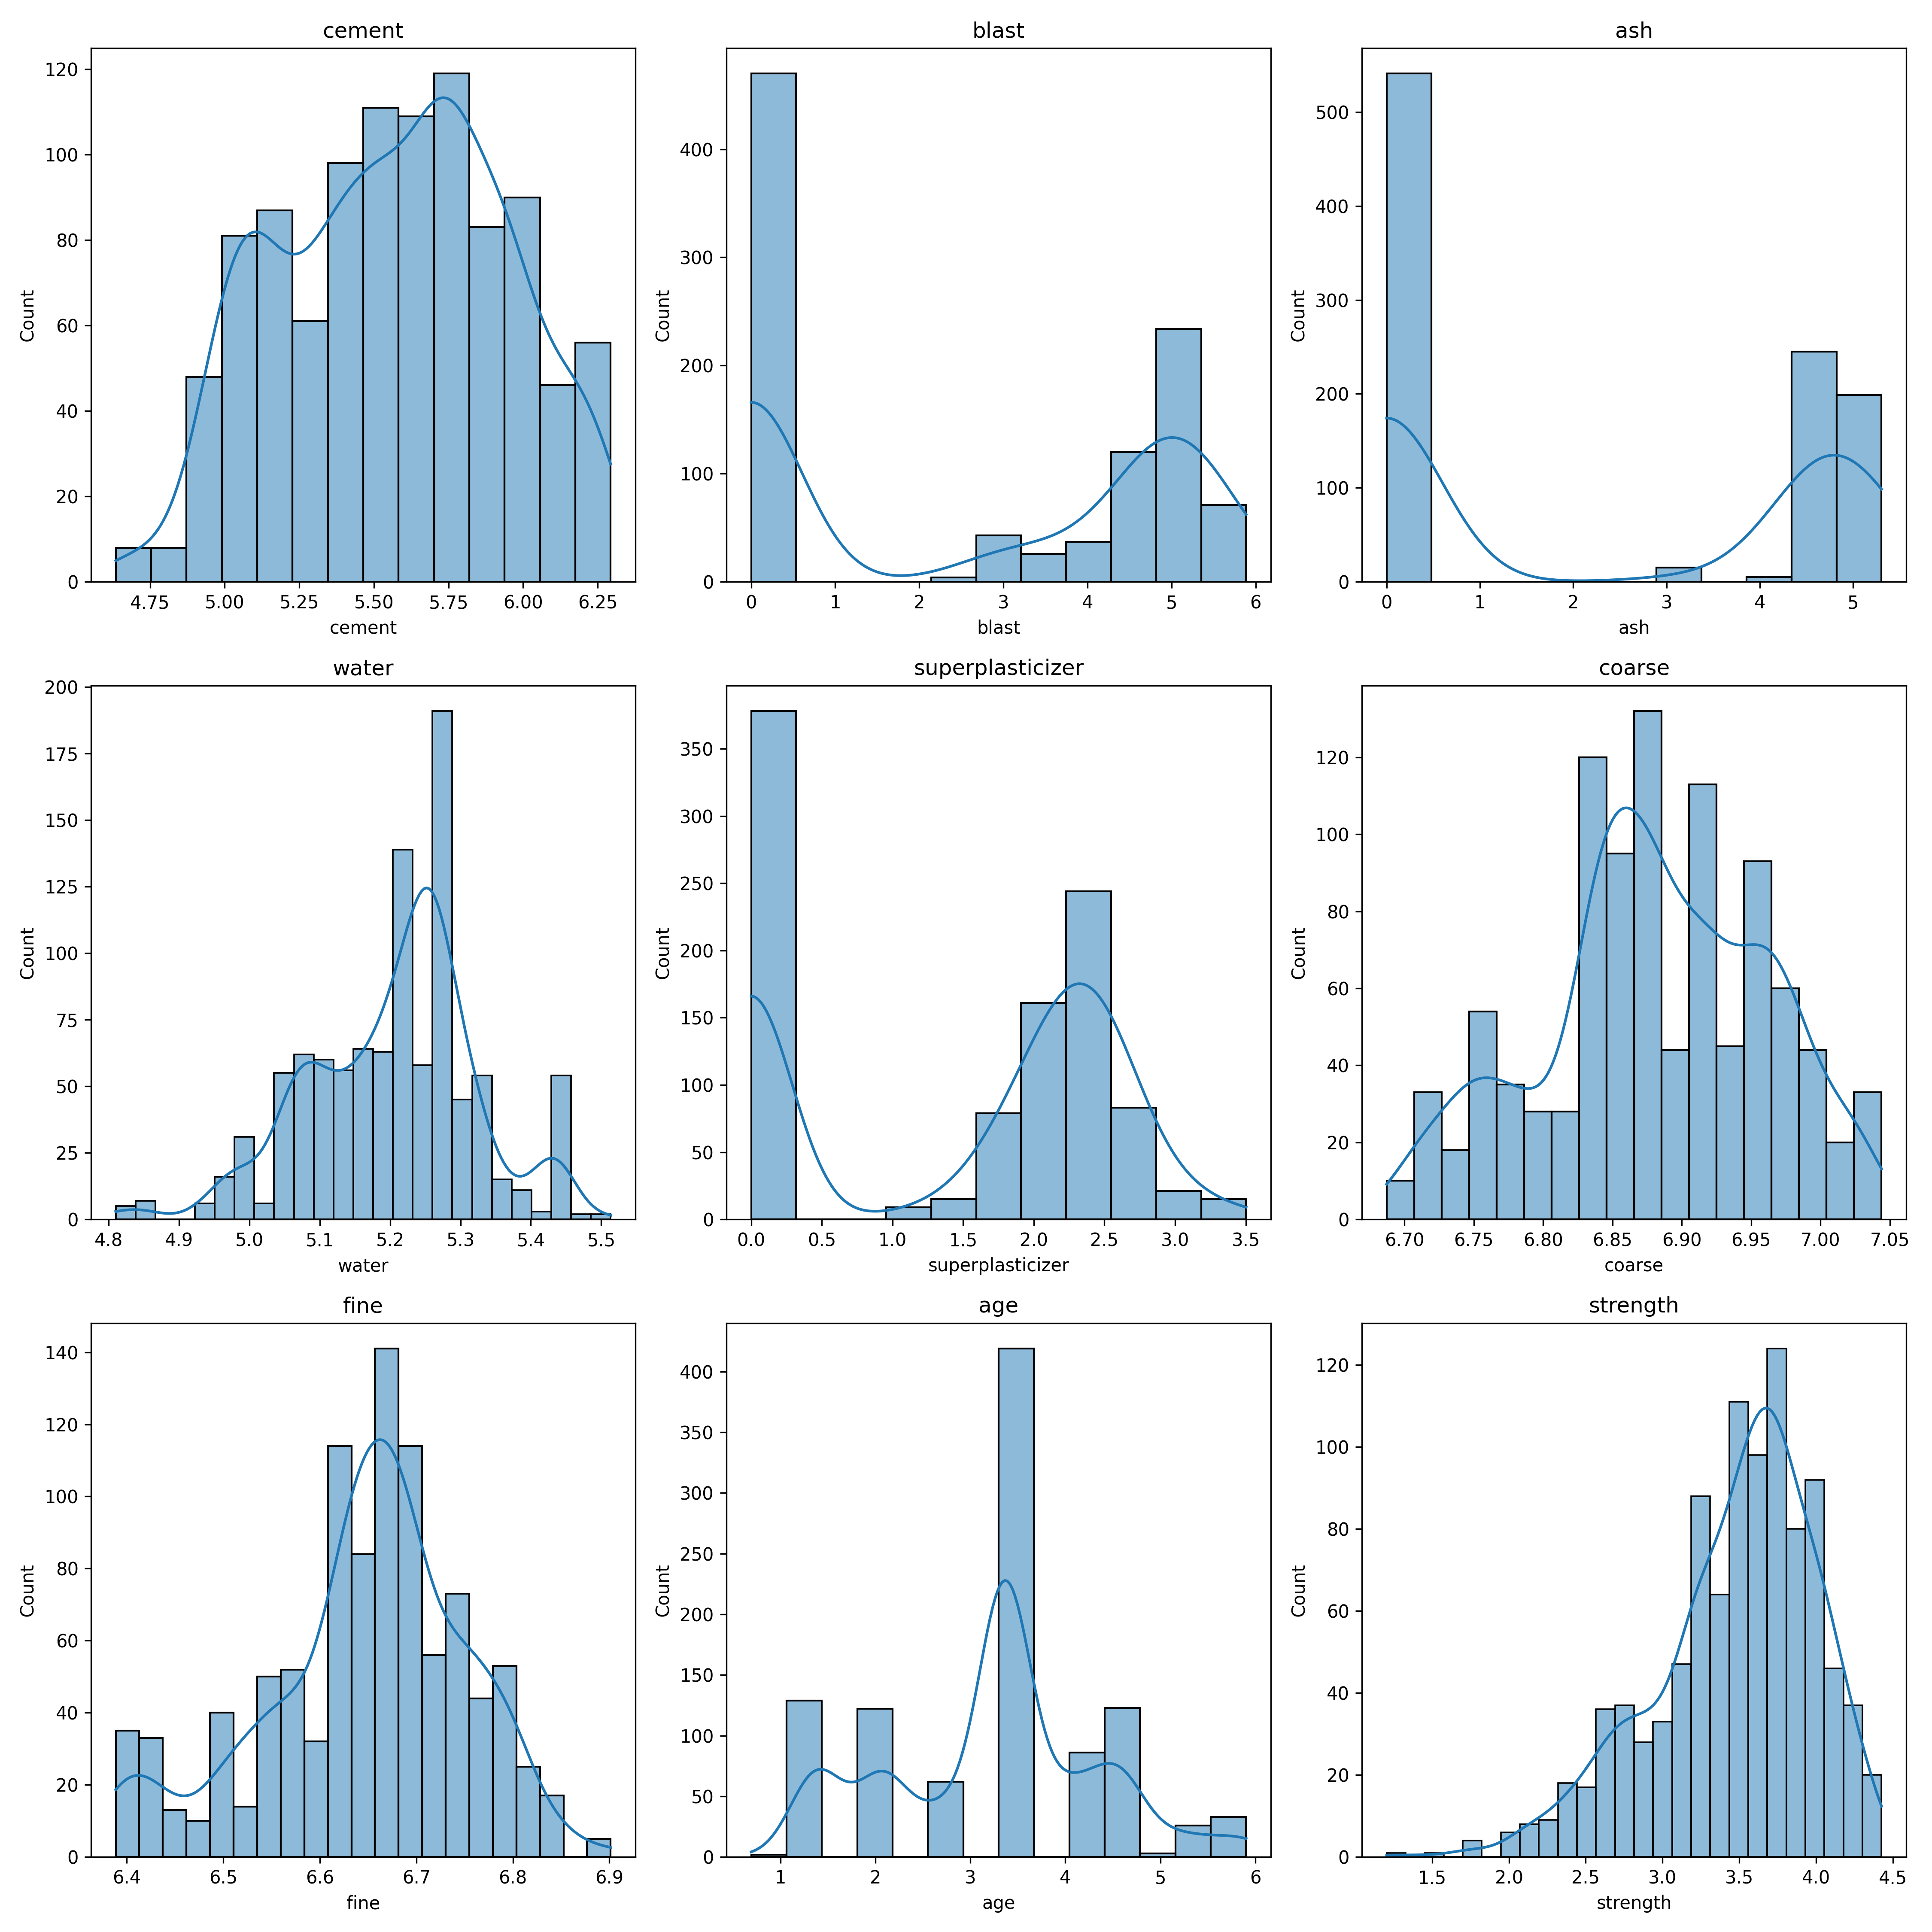
\includegraphics[width=1\textwidth]{../scripts/images/dist.png}
    Quelle: Eigene Darstellung, \ref{linreg}.
    \label{pic:hist}
\end{figure}

Die Korrelationsmatrix, dargestellt in Abbildung \ref{pic:corr}, 
quantifziert die Beziehungen zwischen den einzelnen Bestandteilen des Betons und der Zielvariablen der 
Betondruckfestigkeit. Die Koeffizienten bewegen sich zwischen -0.61 und 0.63, was auf 
unterschiedlich starke Korrelationen hinweist. Ein markantes Beispiel ist der positive Wert 
von 0.63 zwischen Asche und Wasser, was eine starke direkte Beziehung nahelegt, während der Wert 
von -0.61 zwischen Wasser und Superplastifikator auf eine starke umgekehrte Beziehung hindeutet. 
Die Zielvariable der Betondruckfestigkeit zeigt die stärkste direkte Korrelation mit dem Zementgehalt (0.46), 
was darauf schließen lässt, dass ein höherer Zementanteil tendenziell zu einer stärkeren Betonmischung führt. 
Diese Korrelationsmuster sind essentiell für die Modellentwicklung, da sie Aufschluss darüber geben, welche 
Mischungsbestandteile einen bedeutenden Einfluss auf die Betondruckfestigkeit haben könnten.

\begin{figure}[h]
    \caption{Korrelationsmatrix der Merkmale im Datensatz.}
    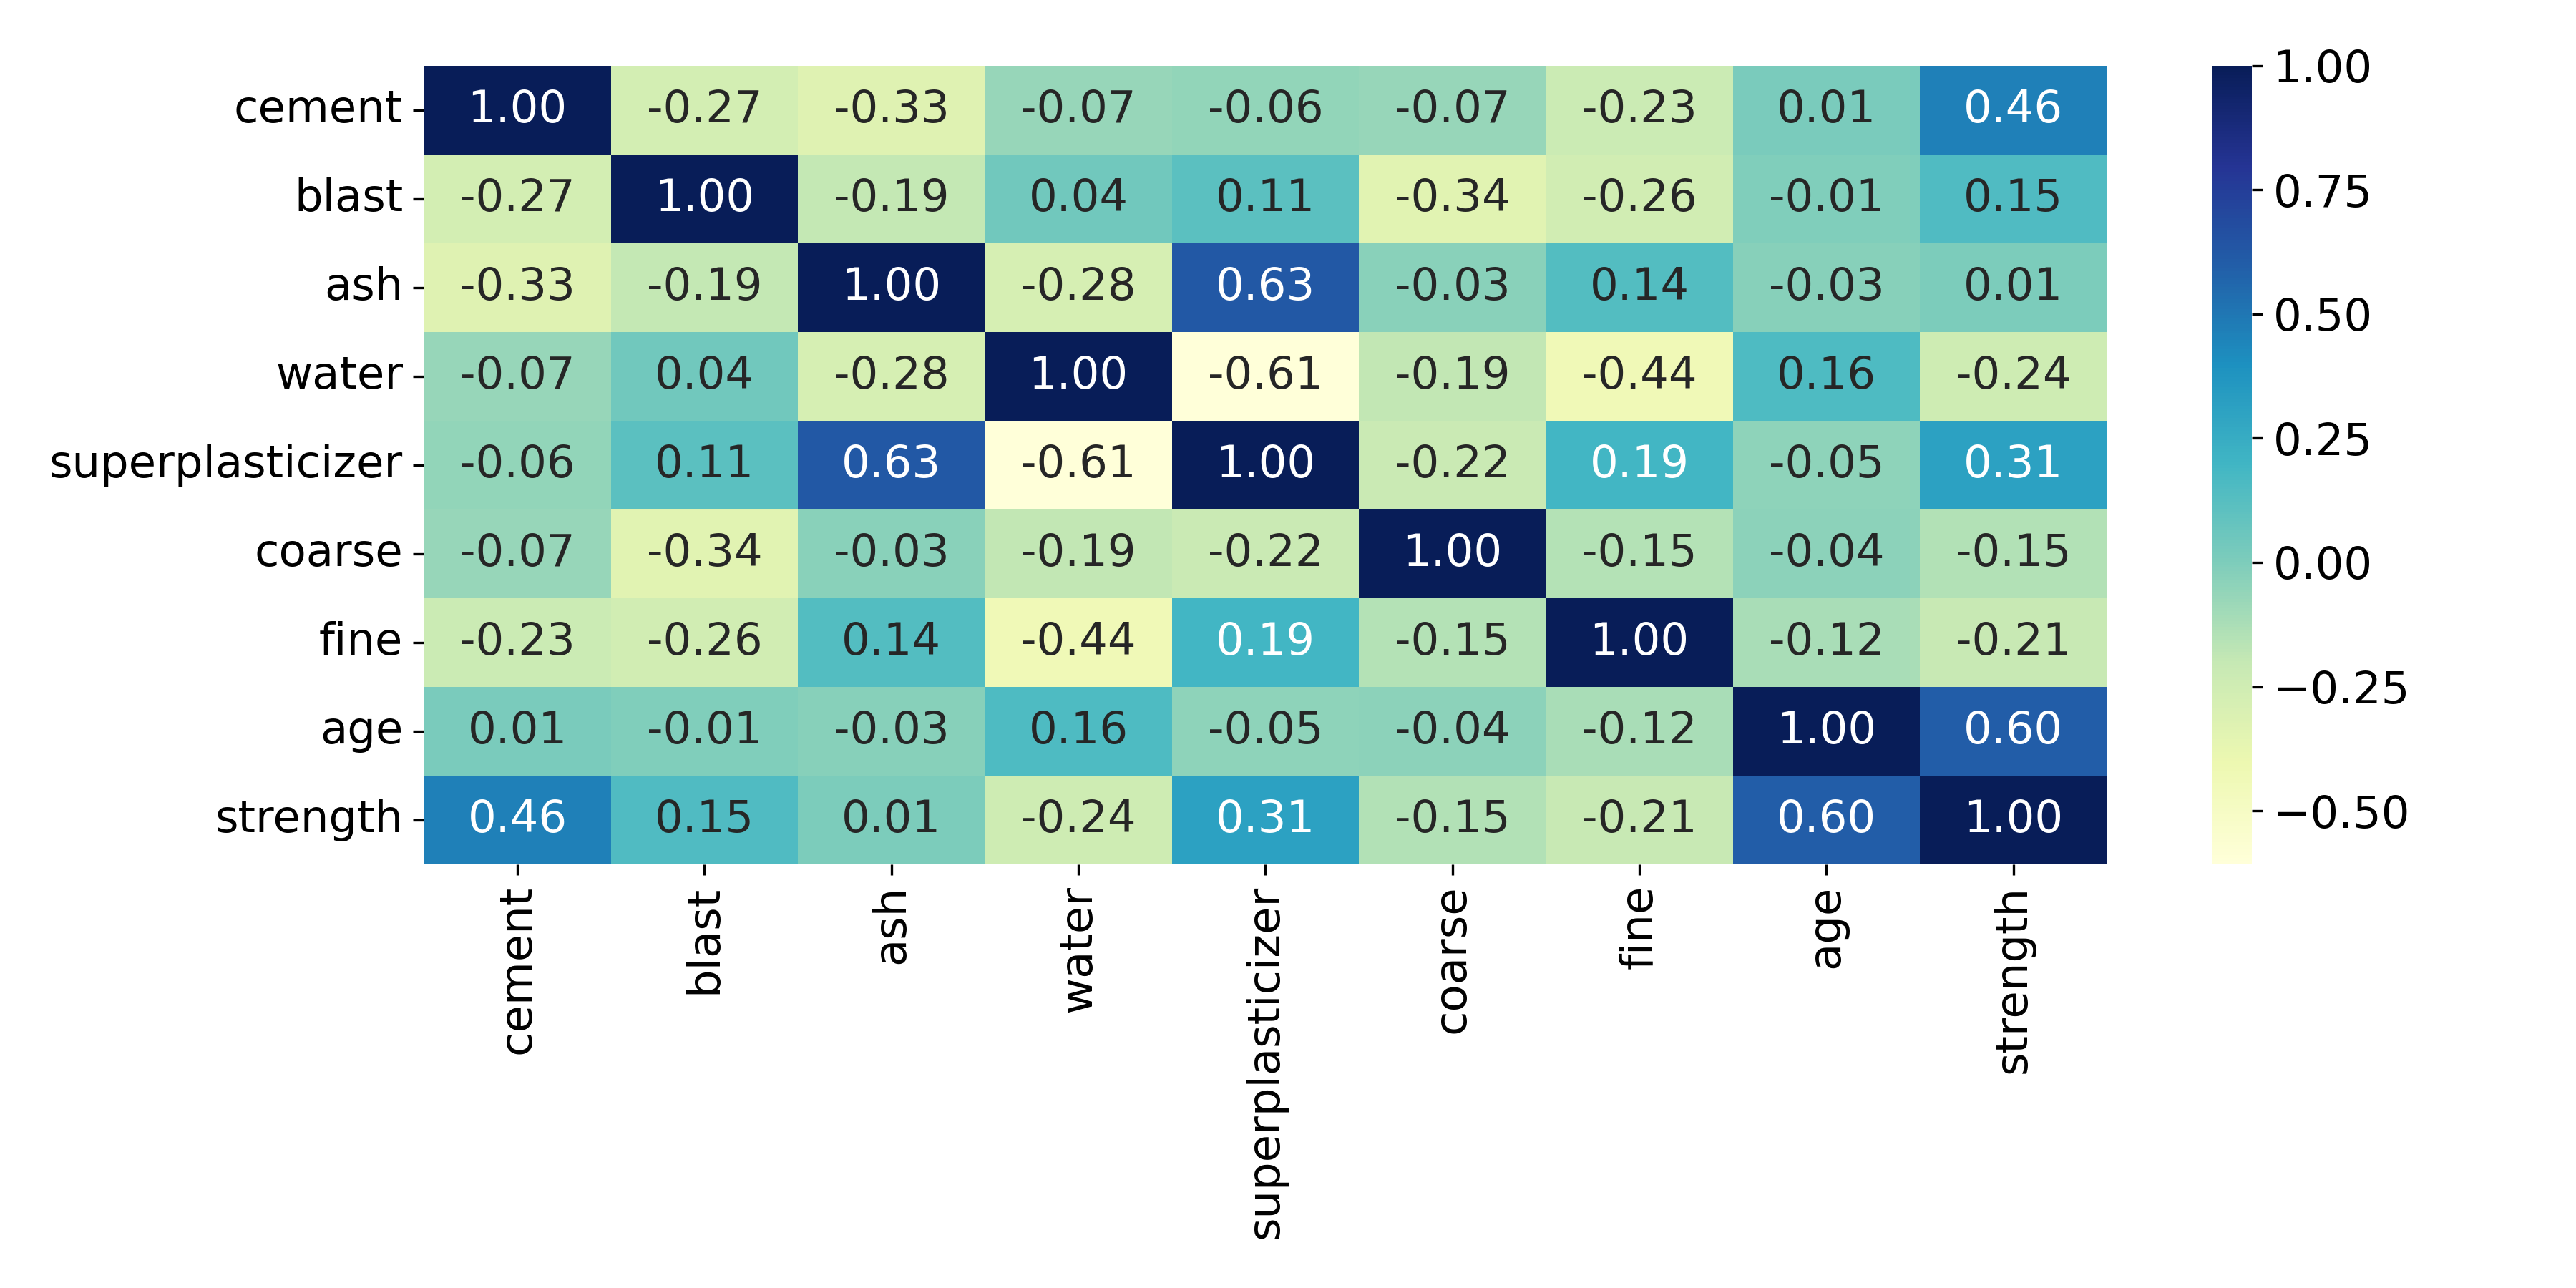
\includegraphics[width=1\textwidth]{../scripts/images/corr.png}
    Quelle: Eigene Darstellung, \ref{linreg}.
    \label{pic:corr}
\end{figure}

\section{Modellierung der linearen Regression}

Um die Beziehung zwischen den unabhängigen Variablen und der Zielvariablen  zu untersuchen, 
wurde ein lineares Regressionsmodell aufgestellt. 
Zur Bewertung der Vorhersageleistung des Modells und zur Vermeidung von Overfitting wurde der 
Datensatz in zwei Teile aufgeteilt: 80\% der Daten dienten als Trainingsset zur 
Anpassung des Modells, während die restlichen 20\% als Testset verwendet wurden, 
um die Modellleistung anhand neuer, unbekannter Daten zu evaluieren. 
Diese Aufteilung erfolgte zufällig, aber reproduzierbar, durch Festlegen eines Seed-Werts 
für den Zufallszahlengenerator, der eine konsistente Teilung des Datensatzes ermöglicht.

Das Trainingsset wurde dazu verwendet, die Koeffizienten der linearen Regression zu schätzen, 
die den Einfluss jeder unabhängigen Variablen auf die Zielvariable quantifizieren. 
Anschließend wurde das Modell mit dem Testset geprüft, um seine Vorhersagegenauigkeit zu bewerten. 
Die Leistung des Modells wurde anhand von Metriken wie dem mittleren quadratischen Fehler (Mean Squared Error, MSE) gemessen, 
die ein Maß für die Abweichung der Modellvorhersagen von den tatsächlichen Werten darstellen.

Codeauschnitt \ref{code:model} und \ref{code:model-train} zeigen das Trainieren und Testen der zugrundeliegenden Daten 
eines linearen Regressionsmodells:

\lstinputlisting[language=Python,label=code:model, firstline=35, lastline=53, 
    caption={Initialisierung eines linearen Regressionsmodells, \ref{linreg}.}, captionpos=top]{../scripts/linreg.py}


\lstinputlisting[language=Python,label=code:model-train, firstline=272, lastline=278, 
    caption={Training und Testen eines linearen Regressionsmodells, \ref{linreg}.}, captionpos=top]{../scripts/linreg.py}


\section{Berechnung von SHAP-Werten}

Um SHAP-Werte zu berechnen, wird zunächst ein SHAP-Explainer-Objekt erstellt. In diesem Fall wird der Explainer 
von SHAP mit dem trainierten linearen Regressionsmodell und dem Trainingsdatensatz initialisiert. 
Anschließend werden die SHAP-Werte für die Testdaten berechnet, um die Beiträge der einzelnen Merkmale 
zu analysieren. Der Typ des Explainers wird durch die Art des übergebenen Modells bestimmt. 
Da in diesem Beispiel ein lineares Modell verwendet wird, wird automatisch ein geeigneter Explainer 
für lineare Modelle ausgewählt.

Das folgende Codeausschnitt \ref{code:shap} zeigt die Initialisierung des SHAP-Explainers und die Berechnung der SHAP-Werte:

\lstinputlisting[language=Python,label=code:shap, firstline=284, lastline=285, 
    caption={Berechnung von SHAP-Werten für das lineare Regressionsmodell, \ref{linreg}.}, captionpos=top]{../scripts/linreg.py}

Das Explainer-Objekt enthält neben den SHAP-Werten (.values), 
die die Einflüsse der einzelnen Merkmale der Testmenge auf die Modellvorhersage quantifizieren, 
auch die Basiswerte (.base\_values), die die durchschnittliche Vorhersage des Modells darstellen, 
und die ursprünglichen Merkmalsausprägungen (.data), die für die Berechnung dieser Werte verwendet wurden \cite[S. 51]{Molnar_2023}.

Dies bildet die Grundlage für den nächsten entscheidenden Schritt: 
die Visualisierung und tiefere Analyse dieser Werte. Die SHAP-Bibliothek bietet eine 
Reihe von leistungsstarken Visualisierungswerkzeugen, die es ermöglichen, die Auswirkungen 
der einzelnen Merkmale auf die Modellvorhersagen intuitiv und verständlich darzustellen. 

Im folgenden Kapitel \ref{chapter:results} werden diese Visualisierungen im Detail vorgestellt. 
Anhand von Beeswarm-Plots, Dependence-Plots und Bar-Plots werden die Ergebnisse der 
SHAP-Analyse dargestellt, die ein umfassendes Bild der Einflüsse und Wichtigkeiten der 
verschiedenen Merkmale im Kontext des linearen Regressionsmodells bieten.

Die Grafiken wurden mithilfe der \textsf{shap}-Bibliothek wie folgt erzeugt:

\lstinputlisting[language=Python,label=code:img, firstline=92, lastline=124, 
    caption={Erzeugen der SHAP Plots, \ref{linreg}.}, captionpos=top]{../scripts/linreg.py}


\chapter{Ergebnisse}
\label{chapter:results}

In diesem Kapitel werden die Resultate der angewandten linearen Regressionsanalyse 
zur Vorhersage der Druckfestigkeit von Beton dargestellt. 
Die Analyse berücksichtigt sowohl die geschätzten Koeffizienten des linearen Modells 
als auch verschiedene Evaluierungsmetriken wie den mittleren absoluten Fehler (MAE), 
den mittleren quadratischen Fehler (MSE) sowie die Bestimmtheitsmaße ($R^2$) 
für Trainings- und Testdaten. Diese Metriken liefern Aufschluss über die Güte des Modells 
und die Präzision der Vorhersagen. Zunächst werden die Koeffizienten 
des linearen Modells auf herkömmliche Weise interpretiert. Anschließend wird gezeigt, 
wie SHAP-Werte eine tiefere und detailliertere Analyse ermöglichen.

\section{Lineares Regressionmodell}

Die Koeffizienten des Modells, die in Tabelle \ref{tab:model-coefficients} 
aufgeführt sind, zeigen, wie stark sich eine Einheitänderung jedes unabhängigen Merkmals 
auf die Beton-Druckfestigkeit auswirkt, unter der Vorraussetzung, dass alle anderen 
Merkmale null sind. 

Positive Koeffizienten deuten auf eine Erhöhung der Beton-Druckfestigkeit 
bei Zunahme der Variablen hin, während negative Koeffizienten eine Verringerung anzeigen. 
Der Intercept-Wert repräsentiert die geschätzte Beton-Druckfestigkeit, 
wenn alle unabhängigen Variablen den Wert Null annehmen. 

Daraus ergibt sich zusammen mit Gleichung \ref{eq:reg-model} die Regressionsgerade für das Modell.

\begin{table}[!h]
    \caption{Koeffizienten des linearen Regressionsmodells}
    \begin{tabularx}{\textwidth}{Xr}
    \toprule
    Merkmal ($\beta_j$) & Koeffizient \\
    \midrule
    Intercept ($\beta_0$) & 4.36596 \\
    cement & 0.75091 \\
    blast & 0.06610 \\
    ash & 0.02683 \\
    water & -0.92315 \\
    superplasticizer & 0.06410 \\
    coarse & 0.08554 \\
    fine &  -0.31901 \\
    age & 0.29090 \\
    \bottomrule
    \end{tabularx}
    \label{tab:model-coefficients}
    \\ Quelle: Eigene Darstellung, \ref{linreg}.
\end{table}

Die Modellmetriken, dargestellt in Tabelle \ref{tab:model-metrics}, 
geben Auskunft über die Vorhersagegenauigkeit und die Anpassungsgüte des Modells. 
Der MAE und RMSE liefern dabei Informationen über die durchschnittliche Größe 
der Fehler in den Vorhersagen, und die $R^2$-Werte zeigen, wie gut das Modell die Varianz 
der Zielvariable erklärt.

\begin{table}[!h]
    \caption{Modellmetriken des linearen Regressionsmodells}
    \begin{tabularx}{\textwidth}{Xr}
    \toprule
    Metrik & Wert \\
    \midrule
    Mean Absolute Error (MAE) & 0.19 \\
    Mean Squared Error (MSE) & 0.06 \\
    Root Mean Squared Error (RMSE) & 0.24 \\
    Training Score (R²) & 0.7852 \\
    Test Score (R²) & 0.8155 \\
    \bottomrule
    \end{tabularx}
    \label{tab:model-metrics}
    \\ Quelle: Eigene Darstellung, \ref{linreg}.
\end{table}

Darüber hinaus wurden die tatsächlichen gegen die vorhergesagten Werte
in Abbildung \ref{pic:residuals} visualisiert, die eine allgemeine Einschätzung der 
Modellgenauigkeit ermöglicht. Ein weiterer wichtiger Aspekt sind die Residuen des Modells. 
Die Residuen, also die Differenzen zwischen den tatsächlichen und vorhergesagten Werten, 
sollten idealerweise zufällig um Null verteilt sein und keine Muster aufweisen, 
die auf eine Verletzung der Modellannahmen hindeuten könnten.

\begin{figure}[!h]
    \caption{Residuenanalyse: Beziehung zwischen Vorhersagen und Abweichungen.}
    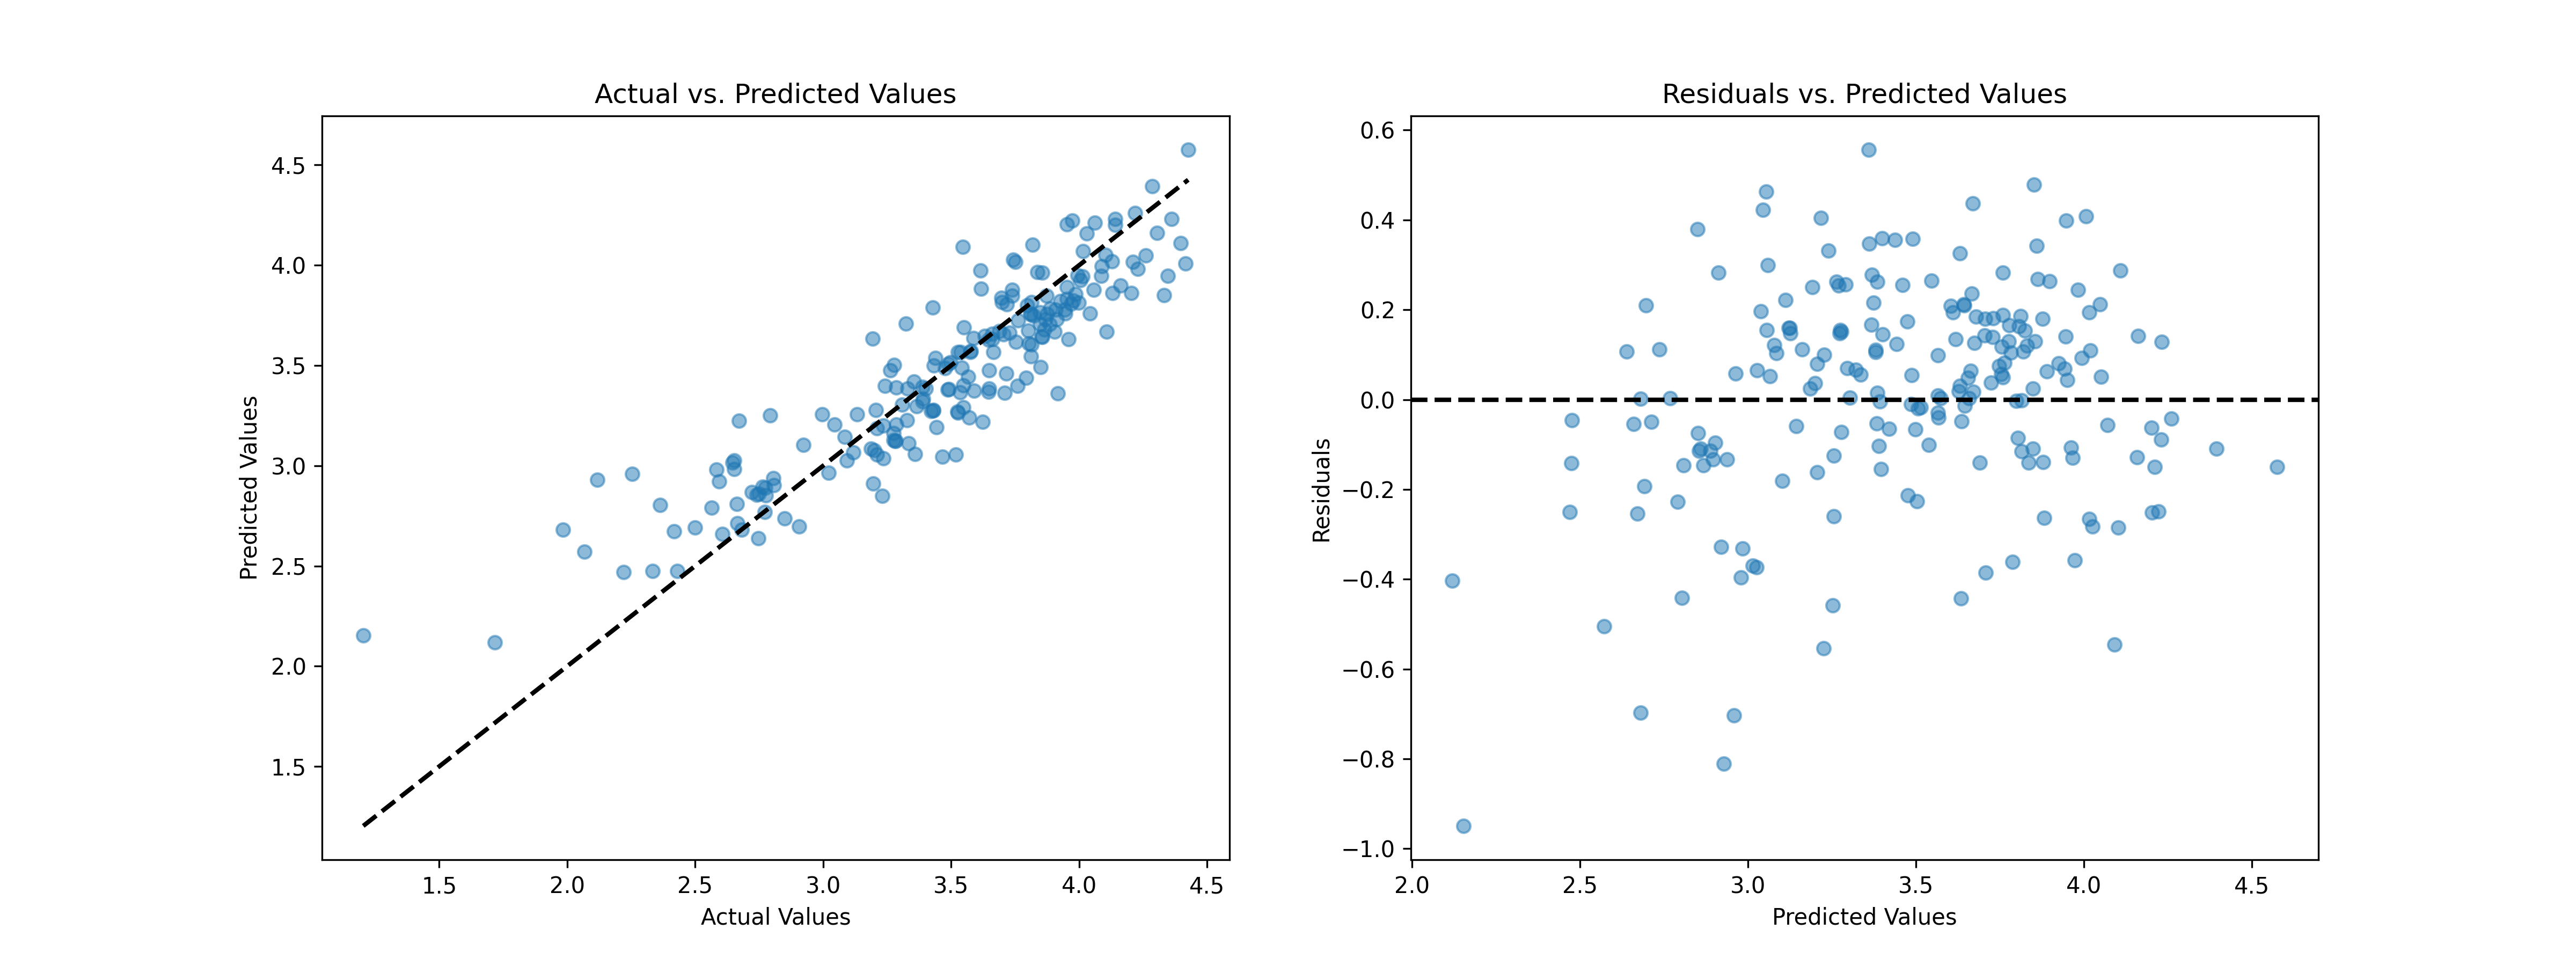
\includegraphics[width=1\textwidth]{../scripts/images/residuals.png}
    Quelle: Eigene Darstellung, \ref{linreg}.
    \label{pic:residuals}
\end{figure}


\section{Interpretation der Koeffizienten \& Permutation Feature Importance}

In diesem Abschnitt wird die herkömmliche Interpretation der Modellkoeffizienten genauer betrachtet. 
Die Koeffizienten eines linearen Modells repräsentieren die Änderung der abhängigen Variable (in diesem Fall die Druckfestigkeit von Beton) 
für eine Einheitänderung der unabhängigen Variablen, unter der Annahme, dass alle anderen Variablen konstant gehalten werden.

Es ist wichtig zu betonen, dass diese Koeffizienten eine bedingte Assoziation beschreiben. 
Das bedeutet, sie quantifizieren die Variation der Druckfestigkeit, wenn eine bestimmte unabhängige Variable 
verändert wird, während alle anderen unabhängigen Variablen konstant gehalten werden. 
Diese Interpretation berücksichtigt die Wechselwirkungen zwischen den verschiedenen unabhängigen Variablen im Modell.

Es ist entscheidend zu verstehen, dass die Koeffizienten nicht als marginale Beiträge betrachtet werden sollten. 
Das bedeutet, sie beschreiben nicht die Beziehung zwischen den Variablen unabhängig von anderen Einflussfaktoren. 
Stattdessen zeigen sie, wie sich die Druckfestigkeit ändert, wenn eine bestimmte unabhängige Variable variiert wird, 
ährend alle anderen konstant gehalten werden.

Abbildung \ref{pic:coef} zeigt die Koeffizienten des Regressionsmodells. Die Stärke des Einflusses einer 
unabhängigen Variable auf die abhängige Variable hängt von der Größe der Merkmalsausprägung ab. 
Ob ein bestimmtes Merkmal einen großen oder kleinen Einfluss auf die abhängige Variable hat, hängt
von den spezifischen Werten der Merkmale und der Streuung der Merkmalsausprägungen ab. 

\begin{figure}[!h]
    \caption{Koeffizienten des linearen Regressionsmodells.}
    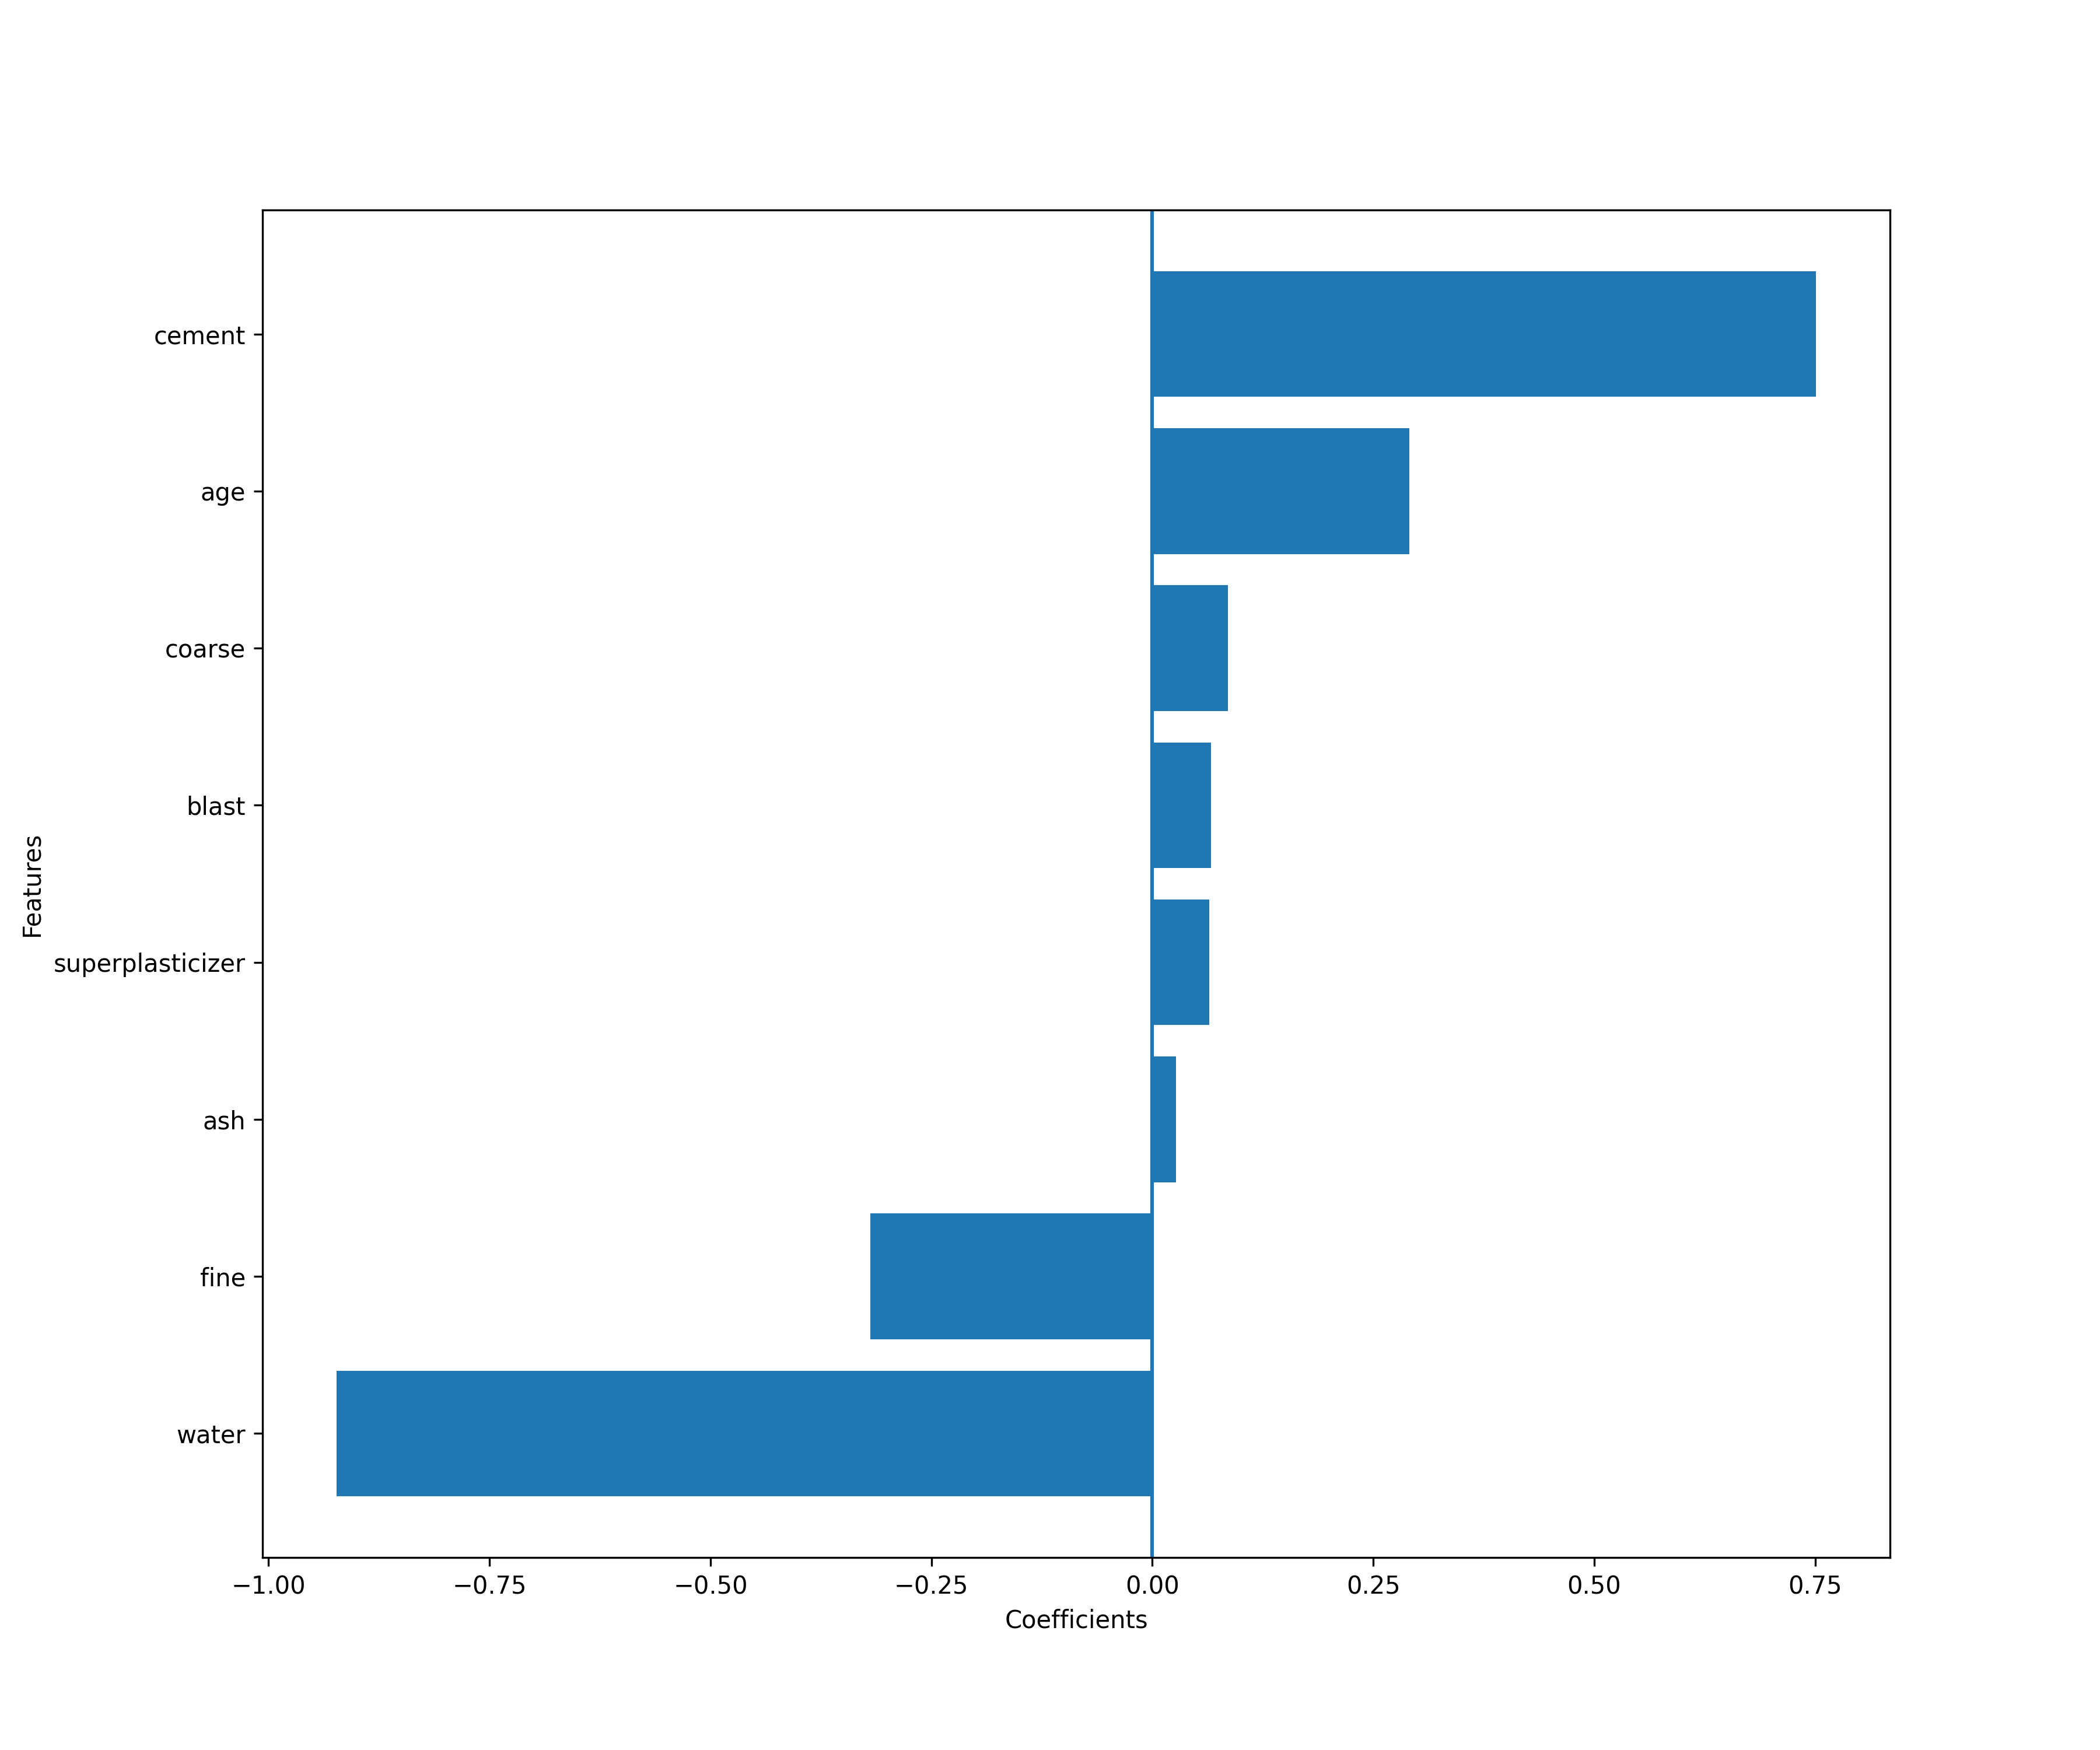
\includegraphics[width=1\textwidth]{../scripts/images/coef.png}
    Quelle: Eigene Darstellung, \ref{linreg}.
    \label{pic:coef}
\end{figure}

Die logarthimische Transformation der Merkmale hat dieses Problem bereits 
teilweise gelöst, indem sie die Skalierung der Daten angepasst hat und alle Merkmale auf eine einheitlichen Skala transformiert hat.
Daraus lassen sich erste Schlüsse der Merkmalsrelevanz ableiten. Im Vergleich zu allen anderen 
Koeffizienten tragen die Merkmale ash, superplasticizer, blast und coarse nur wenig zur abhängigen
Variable bei. 
Das obige Diagramm gibt Aufschluss über die Abhängigkeiten zwischen einem bestimmten Merkmal und der Zielvariablen, 
wenn alle anderen Merkmale konstant bleiben. Eine Erhöhung von cement führt zu einer Erhöhung der Druckfestigkeit. 
Im Gegensatz dazu führt eine Erhöhung von water zu einer Verringerung der Druckfestigkeit, immer unter der Vorraussetzung, das alle
anderen Merkmale konstant bleiben.

Im Anschluss an die Analyse der Koeffizienten des linearen Regressionsmodells wird 
die Feature Importance näher betrachtet. Ein bewährtes Verfahren zur Bestimmung der 
Feature Importance ist die sogenannte Permutation Feature Importance. 
Diese Methode misst die Veränderung im Vorhersagefehler des Modells nach der 
zufälligen Vertauschung der Werte eines bestimmten Merkmals. 
Ein Merkmal gilt als wichtig, wenn die Vertauschung seiner Werte den Modellfehler erhöht, 
da das Modell stark auf dieses Merkmal für seine Vorhersagen angewiesen ist. 
Umgekehrt wird ein Merkmal als unwichtig betrachtet, wenn die Vertauschung seiner Werte 
den Modellfehler unverändert lässt, da das Modell das Merkmal für seine Vorhersagen ignoriert \cite[S. 157]{Molnar_2022}. 

Abbildung \ref{pic:permutation} zeigt die Merkmalsrelevanz auf der Test- und Trainingsmenge 
anhand der Veränderung des mittleren quadratischen Fehlers des Modells:

\begin{figure}[!h]
    \caption{Permutation Feature Importance}
    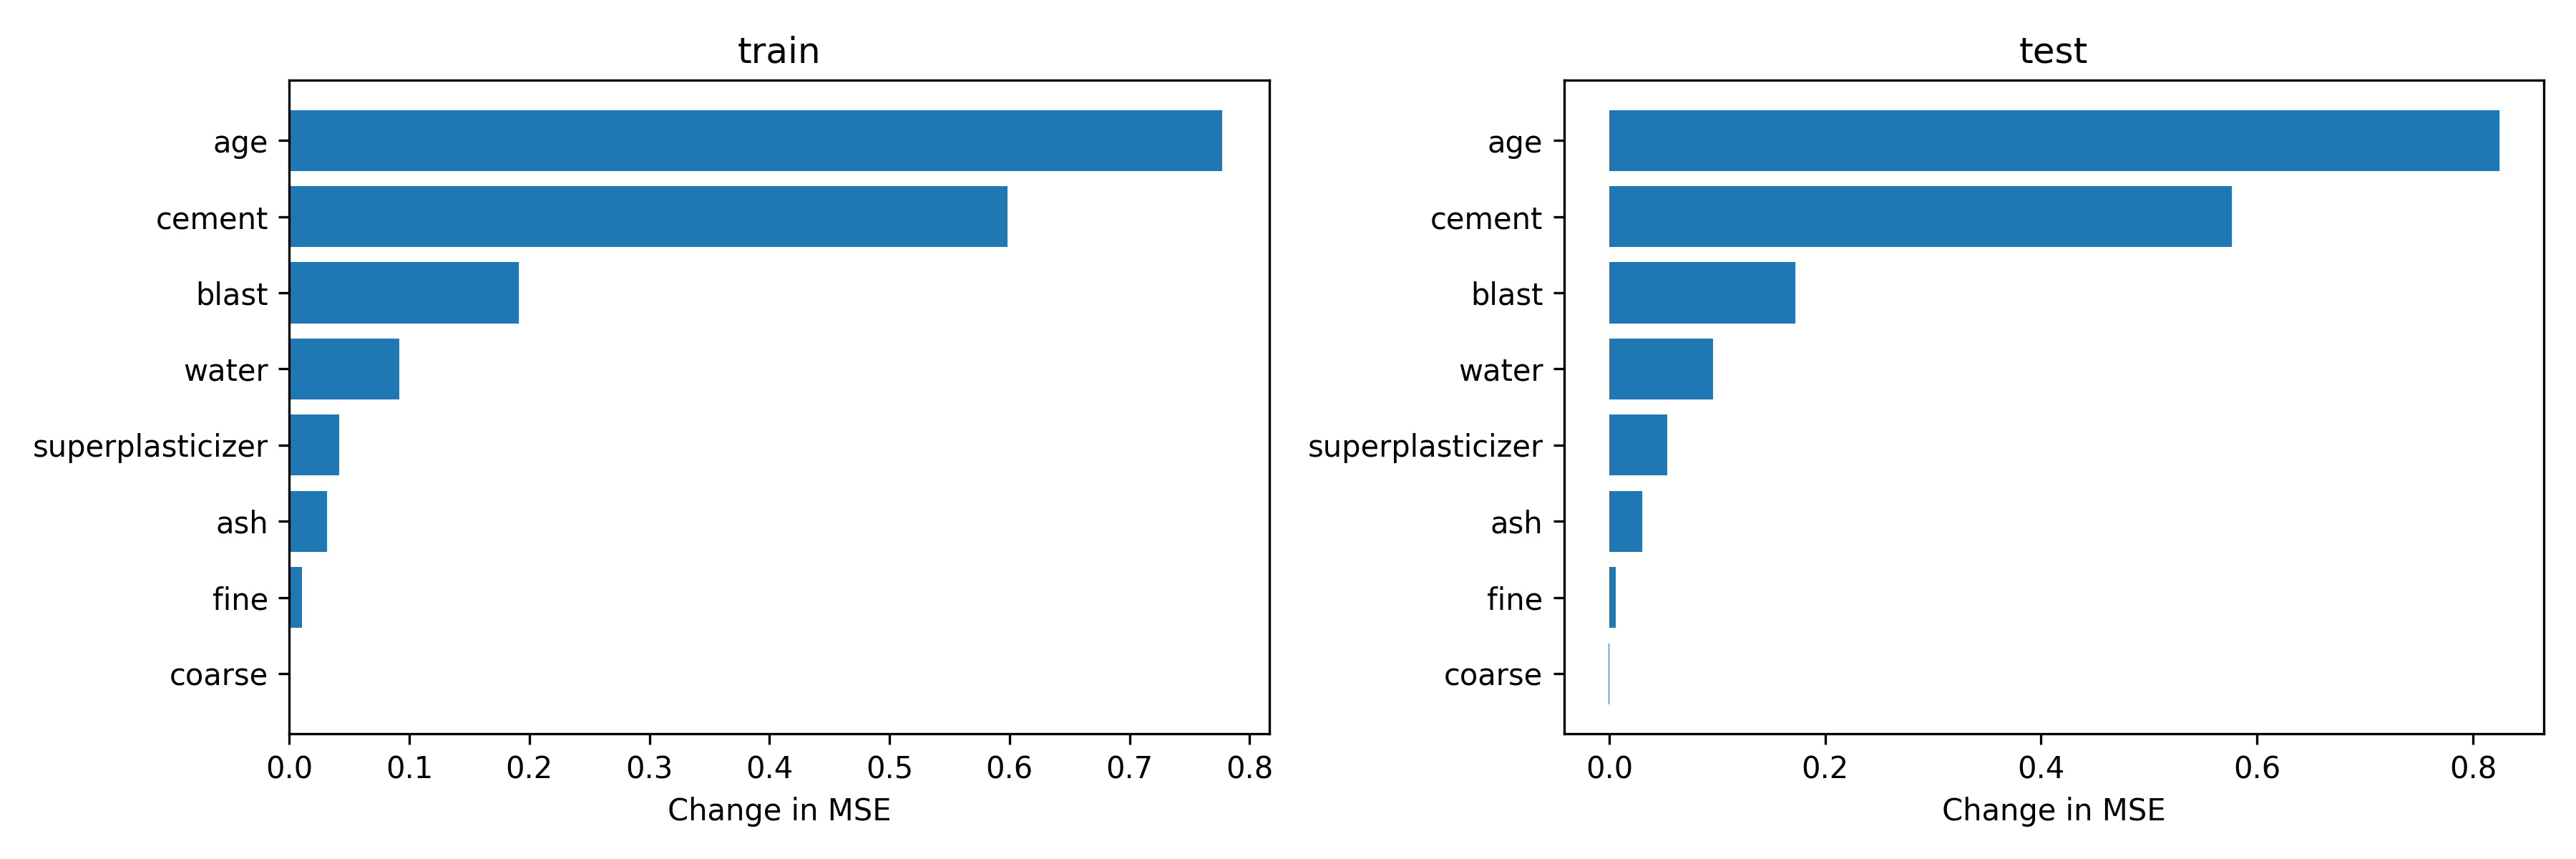
\includegraphics[width=1\textwidth]{../scripts/images/permutation_importance.png}
    Quelle: Eigene Darstellung, \ref{linreg}.
    \label{pic:permutation}
\end{figure}

Es ist festzustellen, dass die Merkmale coarse, fine und ash keine erhebliche Veränderung im mittleren quadratischen
Fehler des Modells hervorrufen und diese somit im Vergleich zu den anderen Merkmalen als eher irrelevant angesehen werden können.

\section{Interpretation mit SHAP}

Durch die Verwendung von SHAP-Werten wird 
es möglich, die Beiträge der einzelnen Merkmale zur Vorhersageleistung des Modells nicht nur 
auf globaler Ebene, sondern auch auf lokaler, individueller Ebene zu verstehen. 
SHAP-Werte berücksichtigen die Wechselwirkungen zwischen den Merkmalen und 
quantifizieren den Beitrag jedes Merkmals zur Abweichung der Prognose im Mittel. 
Dies ermöglicht eine präzisere Interpretation, da die SHAP-Werte den Einfluss 
eines Merkmals auf die Vorhersage unter Berücksichtigung aller anderen Merkmale anzeigen. 

\subsection{Lokale Interpretation}

Die lokale Interpretation konzentriert sich auf das Verständnis der Vorhersagen 
für eine einzelne Beobachtung aus dem Datensatz.

\begin{figure}[!h]
    \caption{SHAP Partial Dependence Plot}
    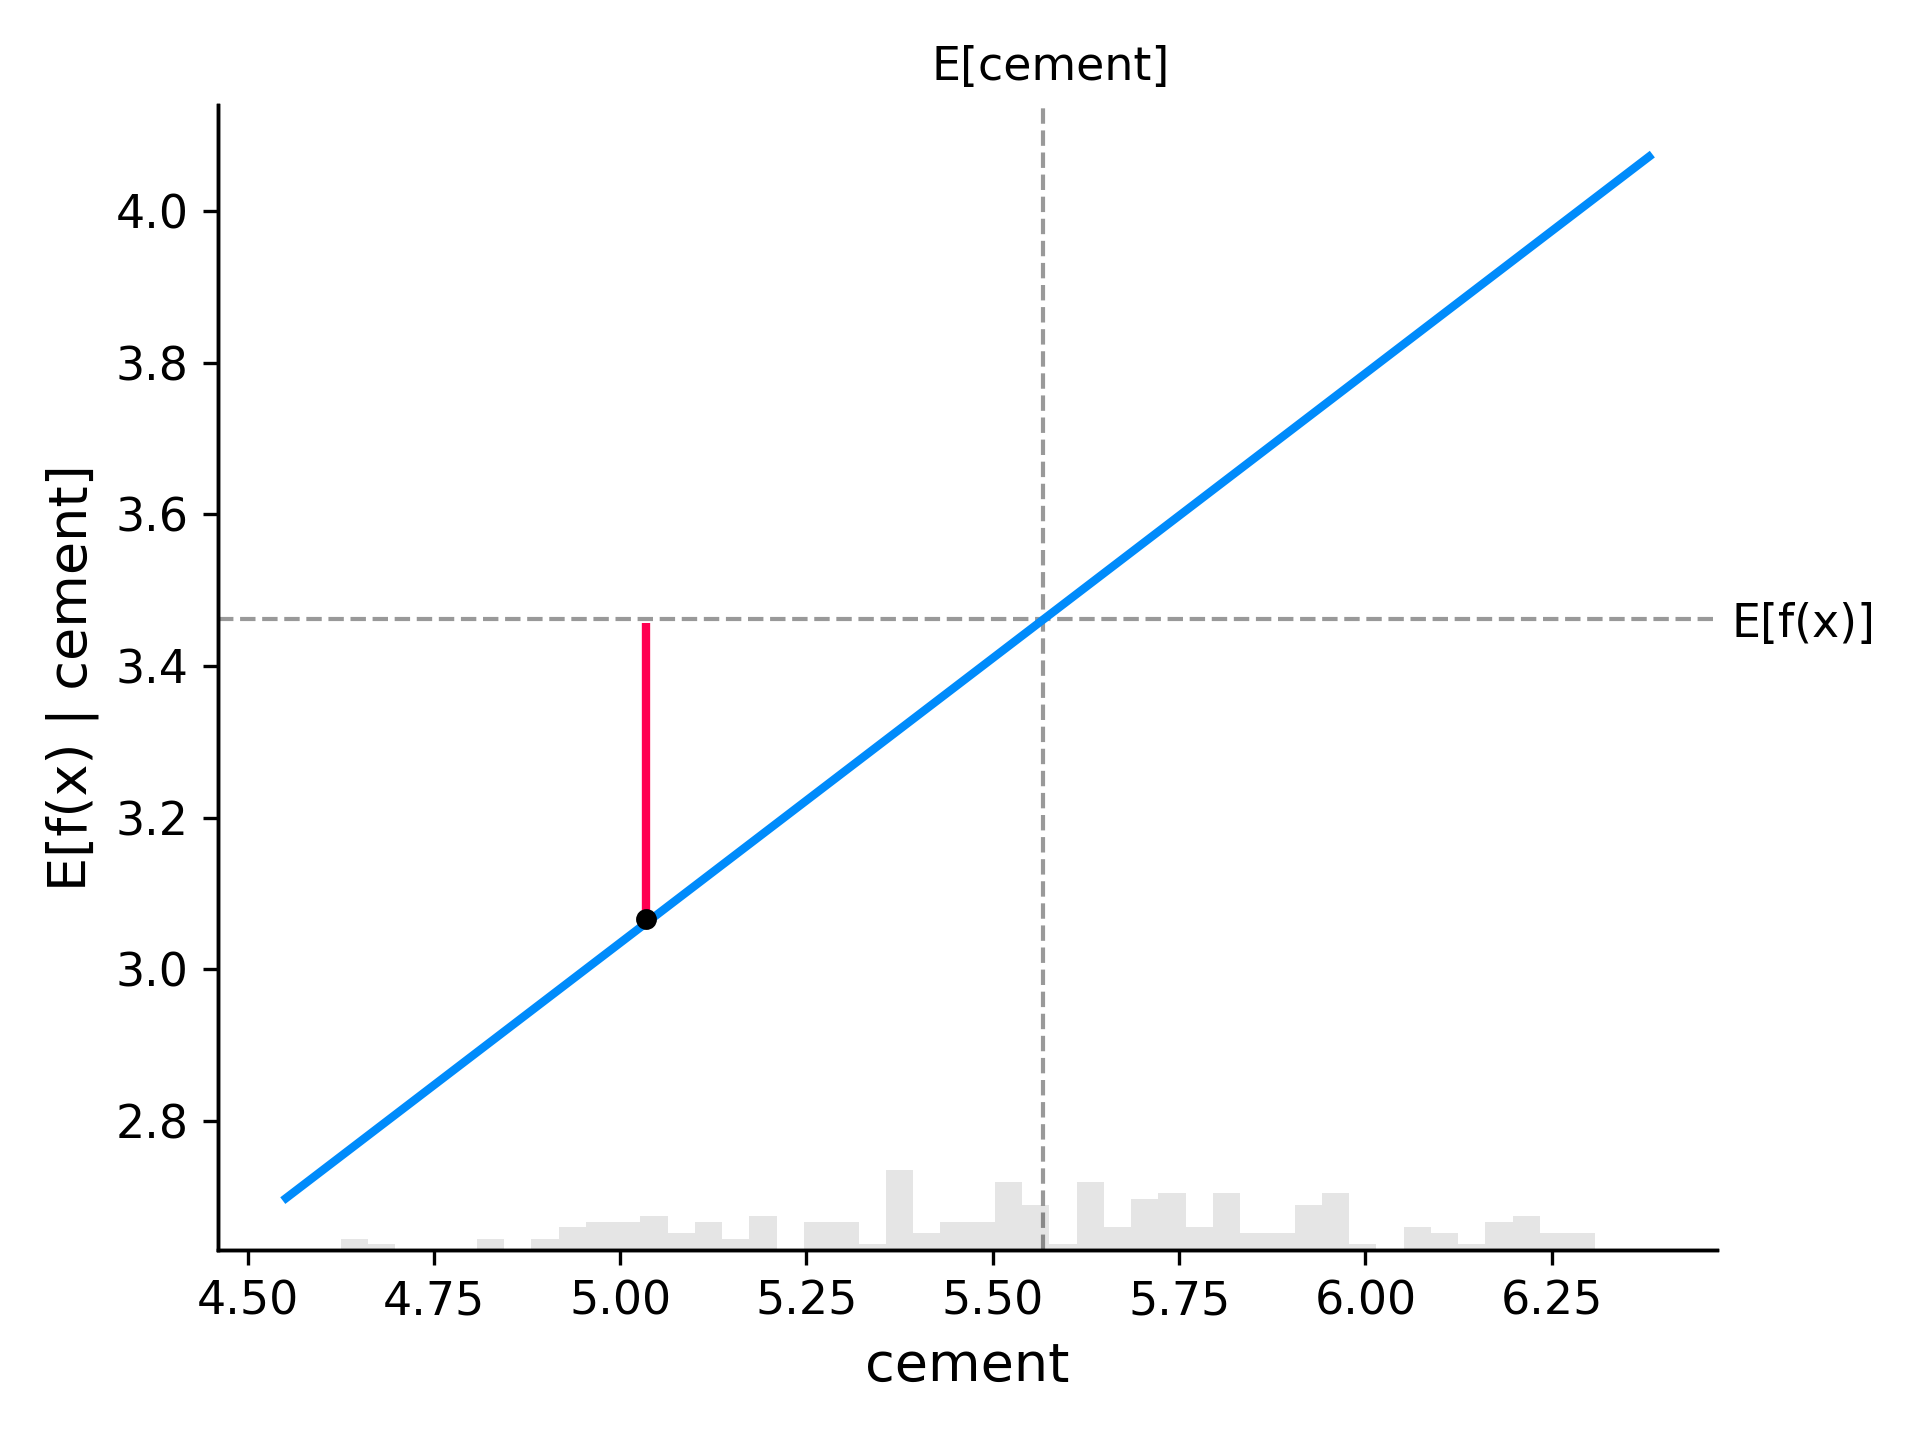
\includegraphics[width=1\textwidth]{../scripts/images/shap_dependence_plot.png}
    Quelle: Eigene Darstellung, \ref{linreg}.
    \label{pic:shap_dependence}
\end{figure}

Im Partial Dependence Plot der Abbildung \ref{pic:shap_dependence} wird die Beziehung zwischen 
dem Merkmal cement und der Zielvariable für die spezifische Beobachtung $x^{(0)}$ aus dem Datensatz visualisiert. 
Die blaue Linie im Diagramm repräsentiert die modellierte Abhängigkeit der Vorhersage vom Merkmal cement, 
unter Konstanthaltung aller anderen Merkmale. Der schwarze Punkt markiert die tatsächliche Ausprägung des 
Merkmals cement ($5.035$) für die betrachtete Beobachtung und die korrespondierende Vorhersage 
des linearen Regressionsmodells. Die rote Linie illustriert die marginale Abweichung der Vorhersage 
von der durchschnittlichen Modellprognose $\mathbb{E}[f(X)] = 3.421$, ausgehend vom beobachteten Wert von cement.

Die Anordnung des schwarzen Punktes entlang der funktionalen Beziehung gibt den spezifischen Wert 
von cement an und reflektiert, wie dieser Wert in den Kontext des gesamten Wertebereichs dieses Merkmals 
eingeordnet wird. Die vertikale Distanz zwischen der durchschnittlichen Vorhersage (dargestellt durch die horizontale 
gestrichelte Linie) und dem Punkt auf der funktionalen Abhängigkeit (blaue Linie) zeigt den Einfluss des Merkmals 
cement auf die individuelle Vorhersage im Vergleich zum Modellmittelwert. Dieser Einfluss verkörpert 
den marginalen Beitrag des Merkmals cement zur Prognoseabweichung für die ausgewählte Beobachtung.

Während der Partial Dependence Plot einen wertvollen Einblick in die Modellabhängigkeit von 
einzelnen Merkmalen bietet, ist für ein umfassendes Verständnis der Modellvorhersage eine ganzheitliche 
Betrachtung aller Merkmale notwendig. Der SHAP Waterfall Plot adressiert diese Notwendigkeit, 
indem er eine kumulative Darstellung aller marginalen Beiträge liefert. Jedes Merkmal wird in 
Form einer Sequenz von Beiträgen visualisiert, beginnend mit dem Basiswert der Vorhersage, welcher 
durch die Addition oder Subtraktion der individuellen Merkmalsbeiträge schrittweise zur finalen Vorhersage 
modifiziert wird.

\begin{figure}[!h]
    \caption{SHAP Waterfall Plot}
    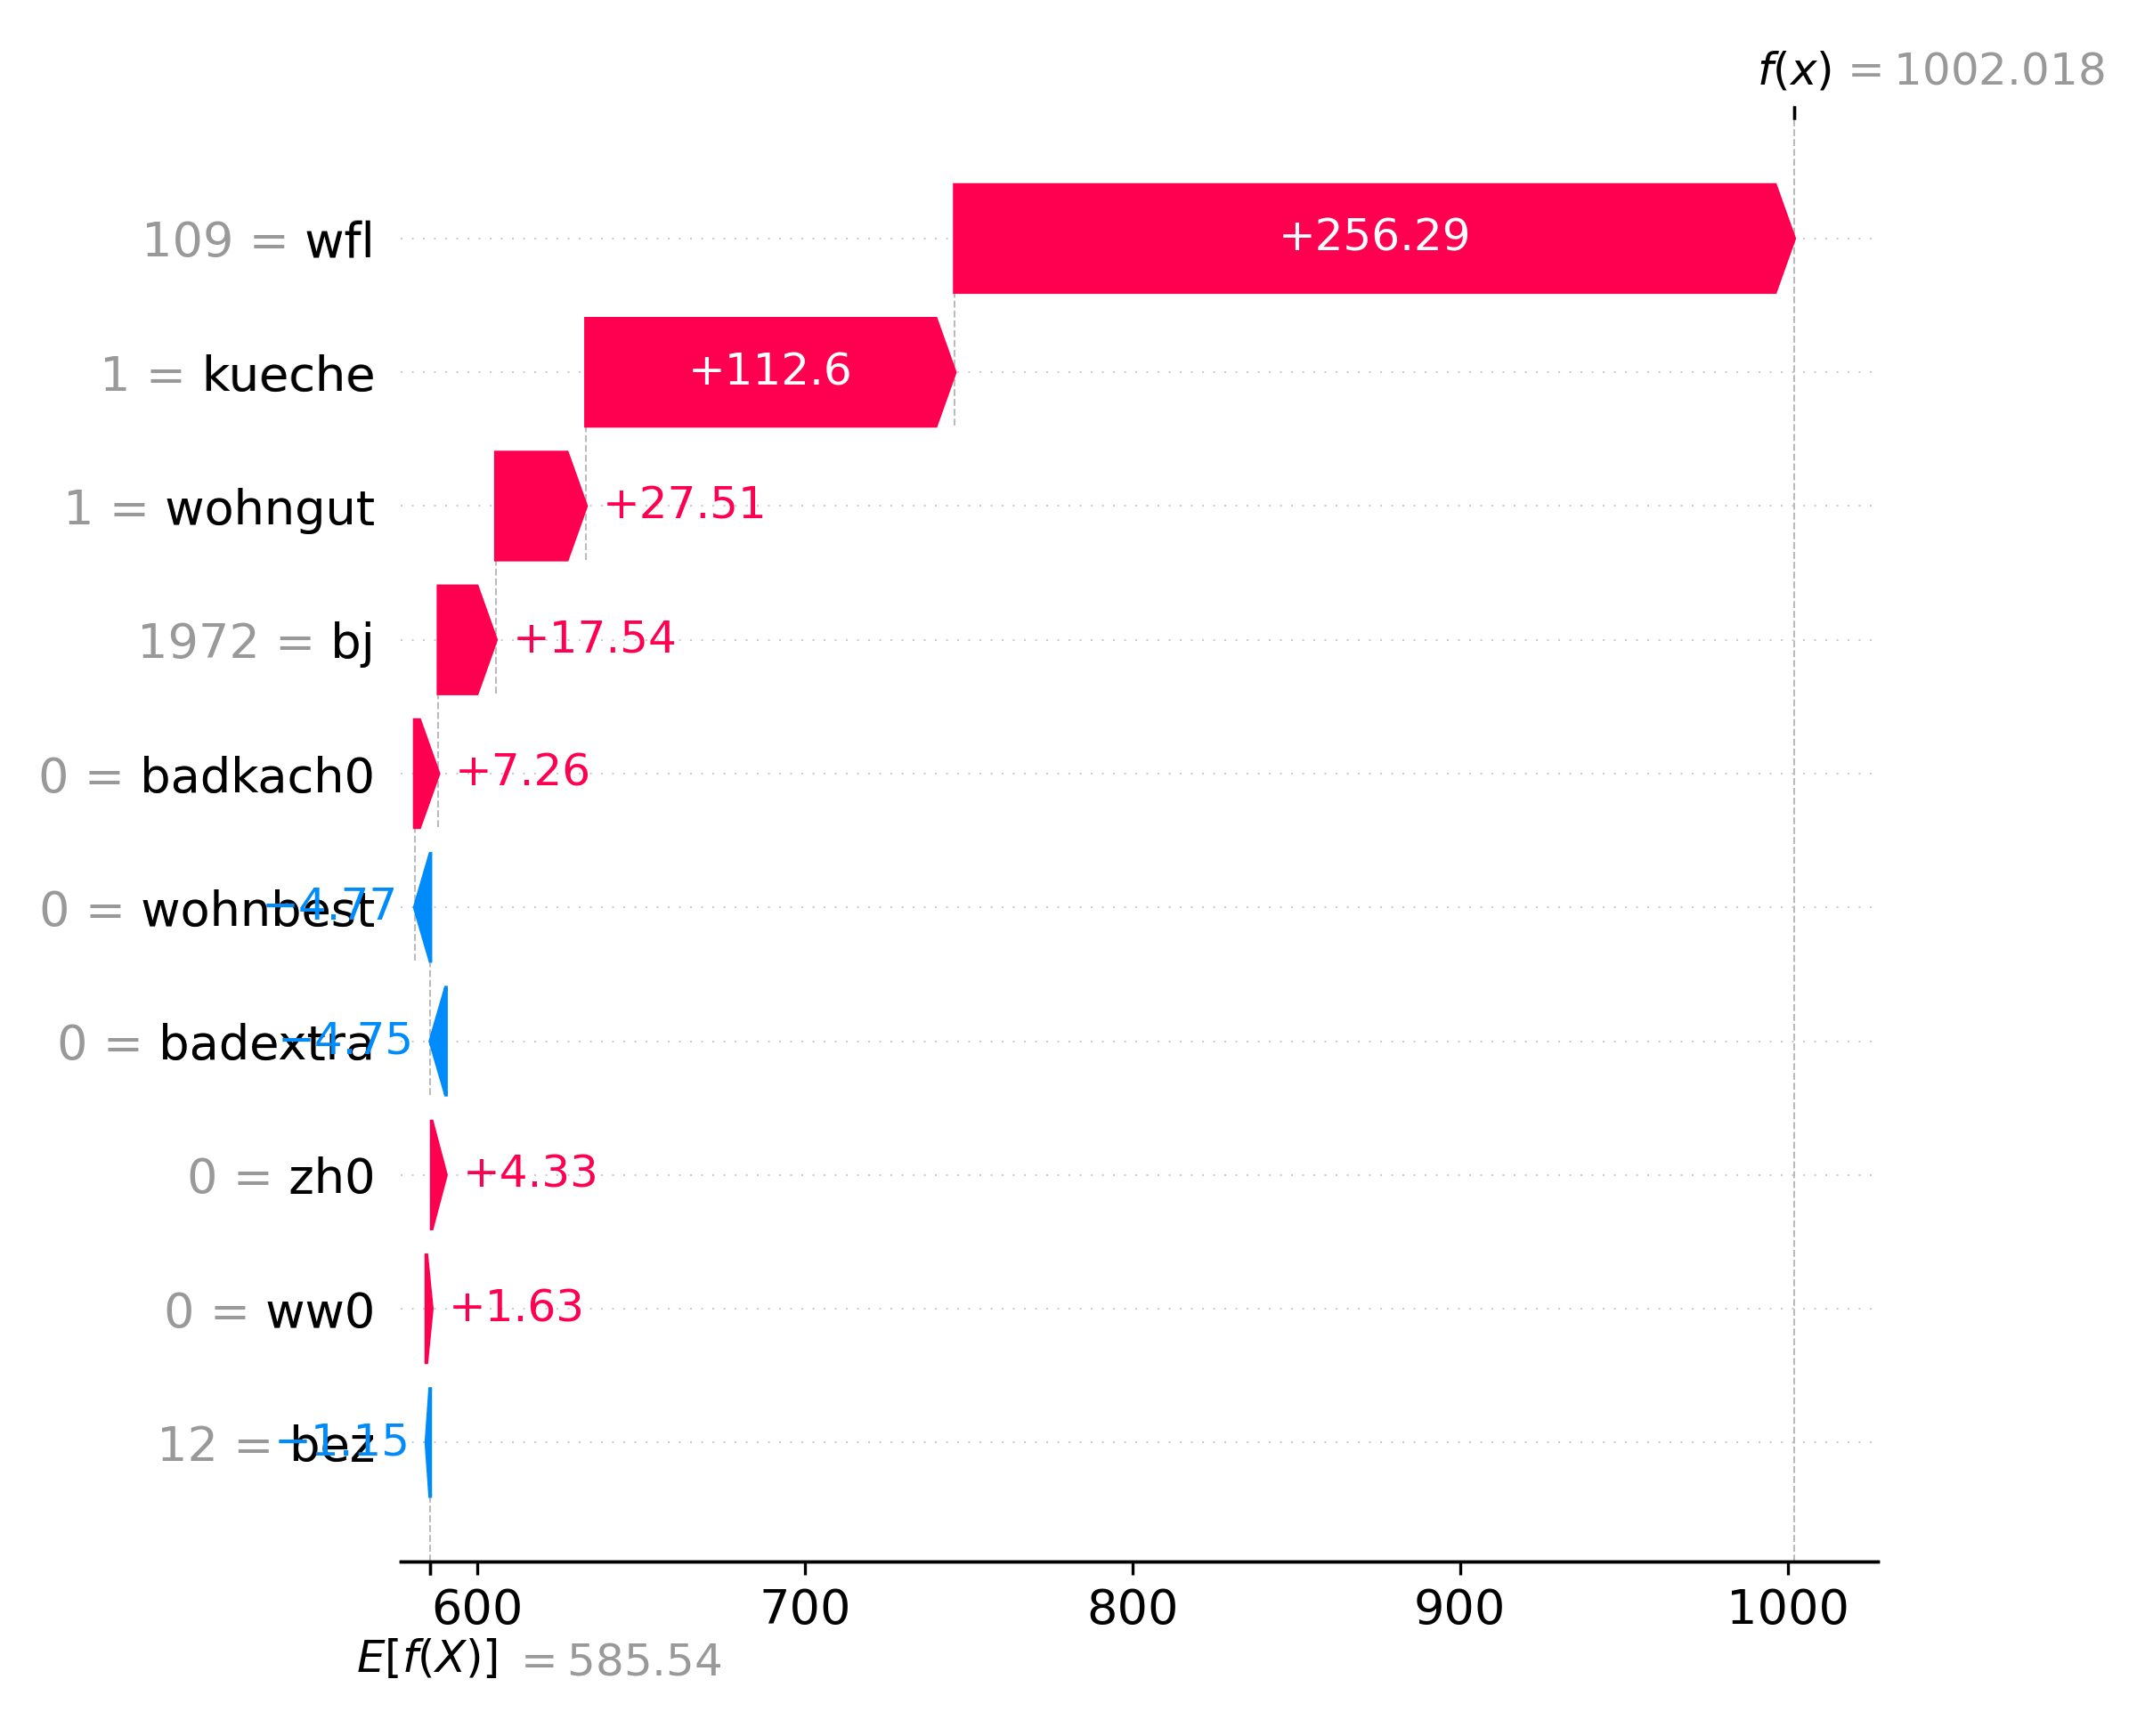
\includegraphics[width=1\textwidth]{../scripts/images/shap_waterfall_plot.png}
    Quelle: Eigene Darstellung, \ref{linreg}.
    \label{pic:shap_waterfall}
\end{figure}

In Abbildung \ref{pic:shap_waterfall} ist ein Waterfall Plot der ersten Beobachtung $x^{(0)}$ dargestellt, 
der die Zerlegung einer einzelnen Modellvorhersage zeigt. Der Plot beginnt mit dem Basiswert $\mathbb{E}[f(X)] = 3.421$, 
der durchschnittlichen Vorhersage des Modells. 

Von diesem Wert ausgehend, illustrieren die Balken, wie jede Merkmalausprägung – 
angezeigt durch die grauen Zahlen entlang der y-Achse – die Vorhersage $f(x_{j}^{(0)})$ beeinflusst. 
So steigert beispielsweise blast mit einem Wert von $4.982$ die Vorhersage um $+0.21$, 
wohingegen cement mit einem Wert von $5.035$ die Vorhersage um $-0.45$ verringert.

Rote Balken repräsentieren Merkmale, die die Vorhersage erhöhen, während blaue Balken solche 
darstellen, die sie senken. Die Größe jedes Balkens zeigt das Ausmaß des jeweiligen Beitrags, 
und die abschließende Vorhersage $f(x) = 3.257$ wird am Ende der Kette dieser Effekte erreicht. 

Kleine positive und negative Beiträge von Merkmalen wie fine ($6.713$), water ($5.188$), ash ($0$) und superplasticizer ($2.197$) 
zeigen, wie feingranulare Anpassungen der Merkmalsausprägungen die Vorhersage leicht erhöhen oder senken können.

Für die Beobachtung $x^{(0)}$ führt die kumulative Abweichung der Merkmal-Effekte 
vom Basiswert $\mathbb{E}[f(X)] = 3.421$ zu einem tatsächlichen Modelloutput von $f(x) = 3.257$, 
was eine Differenz von $-0.164$ zwischen der durchschnittlichen Vorhersage 
und der spezifischen Vorhersage für diese Beobachtung offenlegt. 
Diese Differenz entspricht der Summe aller SHAP-Werte für diese konkrete Beobachtung \cite[S. 52f]{Molnar_2023}.

Da die Zielgröße einer logarithmischen Transformation unterzogen wurde, muss diese für die Interpreation wieder rückgängig gemacht werden. 
Dies bedeutet, dass der tatsächliche erwartete Wert der Druckfestigkeit der Exponentialfunktion des prognostizierten Wertes entspricht, also $e^{3.421} \approx 30.60$ MPa. 
Dieser Rücktransformationsprozess ist notwendig, um die Modellprognosen in der ursprünglichen Skala der Zielvariablen zu interpretieren.
Dies gilt darüberhinaus sowhl für die einzelnen SHAP-Werte, als auch für die konkrete Vorhersage $f(x) = 3.257$. 
Die prognostizierte Durckfestigkeit für die Beobachtung $x^{(0)}$ beträgt folglich $e^{3.257} \approx 25.97$ MPa.

Dies ermöglicht eine detaillierte Analyse, wie das Modell zu einer bestimmten Vorhersage kommt, 
und hilft dabei, die Beiträge und Interaktionen zwischen verschiedenen Merkmalen zu verstehen.

Die lokale Interpretation mittels SHAP-Werten ermöglicht zwar eine präzise Erklärung 
der Modellvorhersagen für individuelle Beobachtungen, jedoch stellt sich bei einer 
solchen Betrachtung das Problem der fehlenden Generalisierbarkeit. 
Lokale Analysen können dazu führen, dass spezifische Merkmal-Kontributionen überinterpretiert werden, 
ohne die übergeordneten Muster und Einflüsse zu berücksichtigen, 
die das Modellverhalten im gesamten Datensatz charakterisieren. 
Eine globale Interpretation ist daher erforderlich, um die Konsistenz und Zuverlässigkeit 
des Modells über verschiedene Beobachtungen hinweg zu erfassen. 

\subsection{Globale Interpretation}

Der folgende Abschnitt widmet sich dieser globalen Sichtweise und untersucht, 
wie die Merkmalsa-Beiträge sich im Kontext des gesamten Datensatzes darstellen lassen.

\begin{figure}[!h]
    \caption{SHAP Beeswarm Plot}
    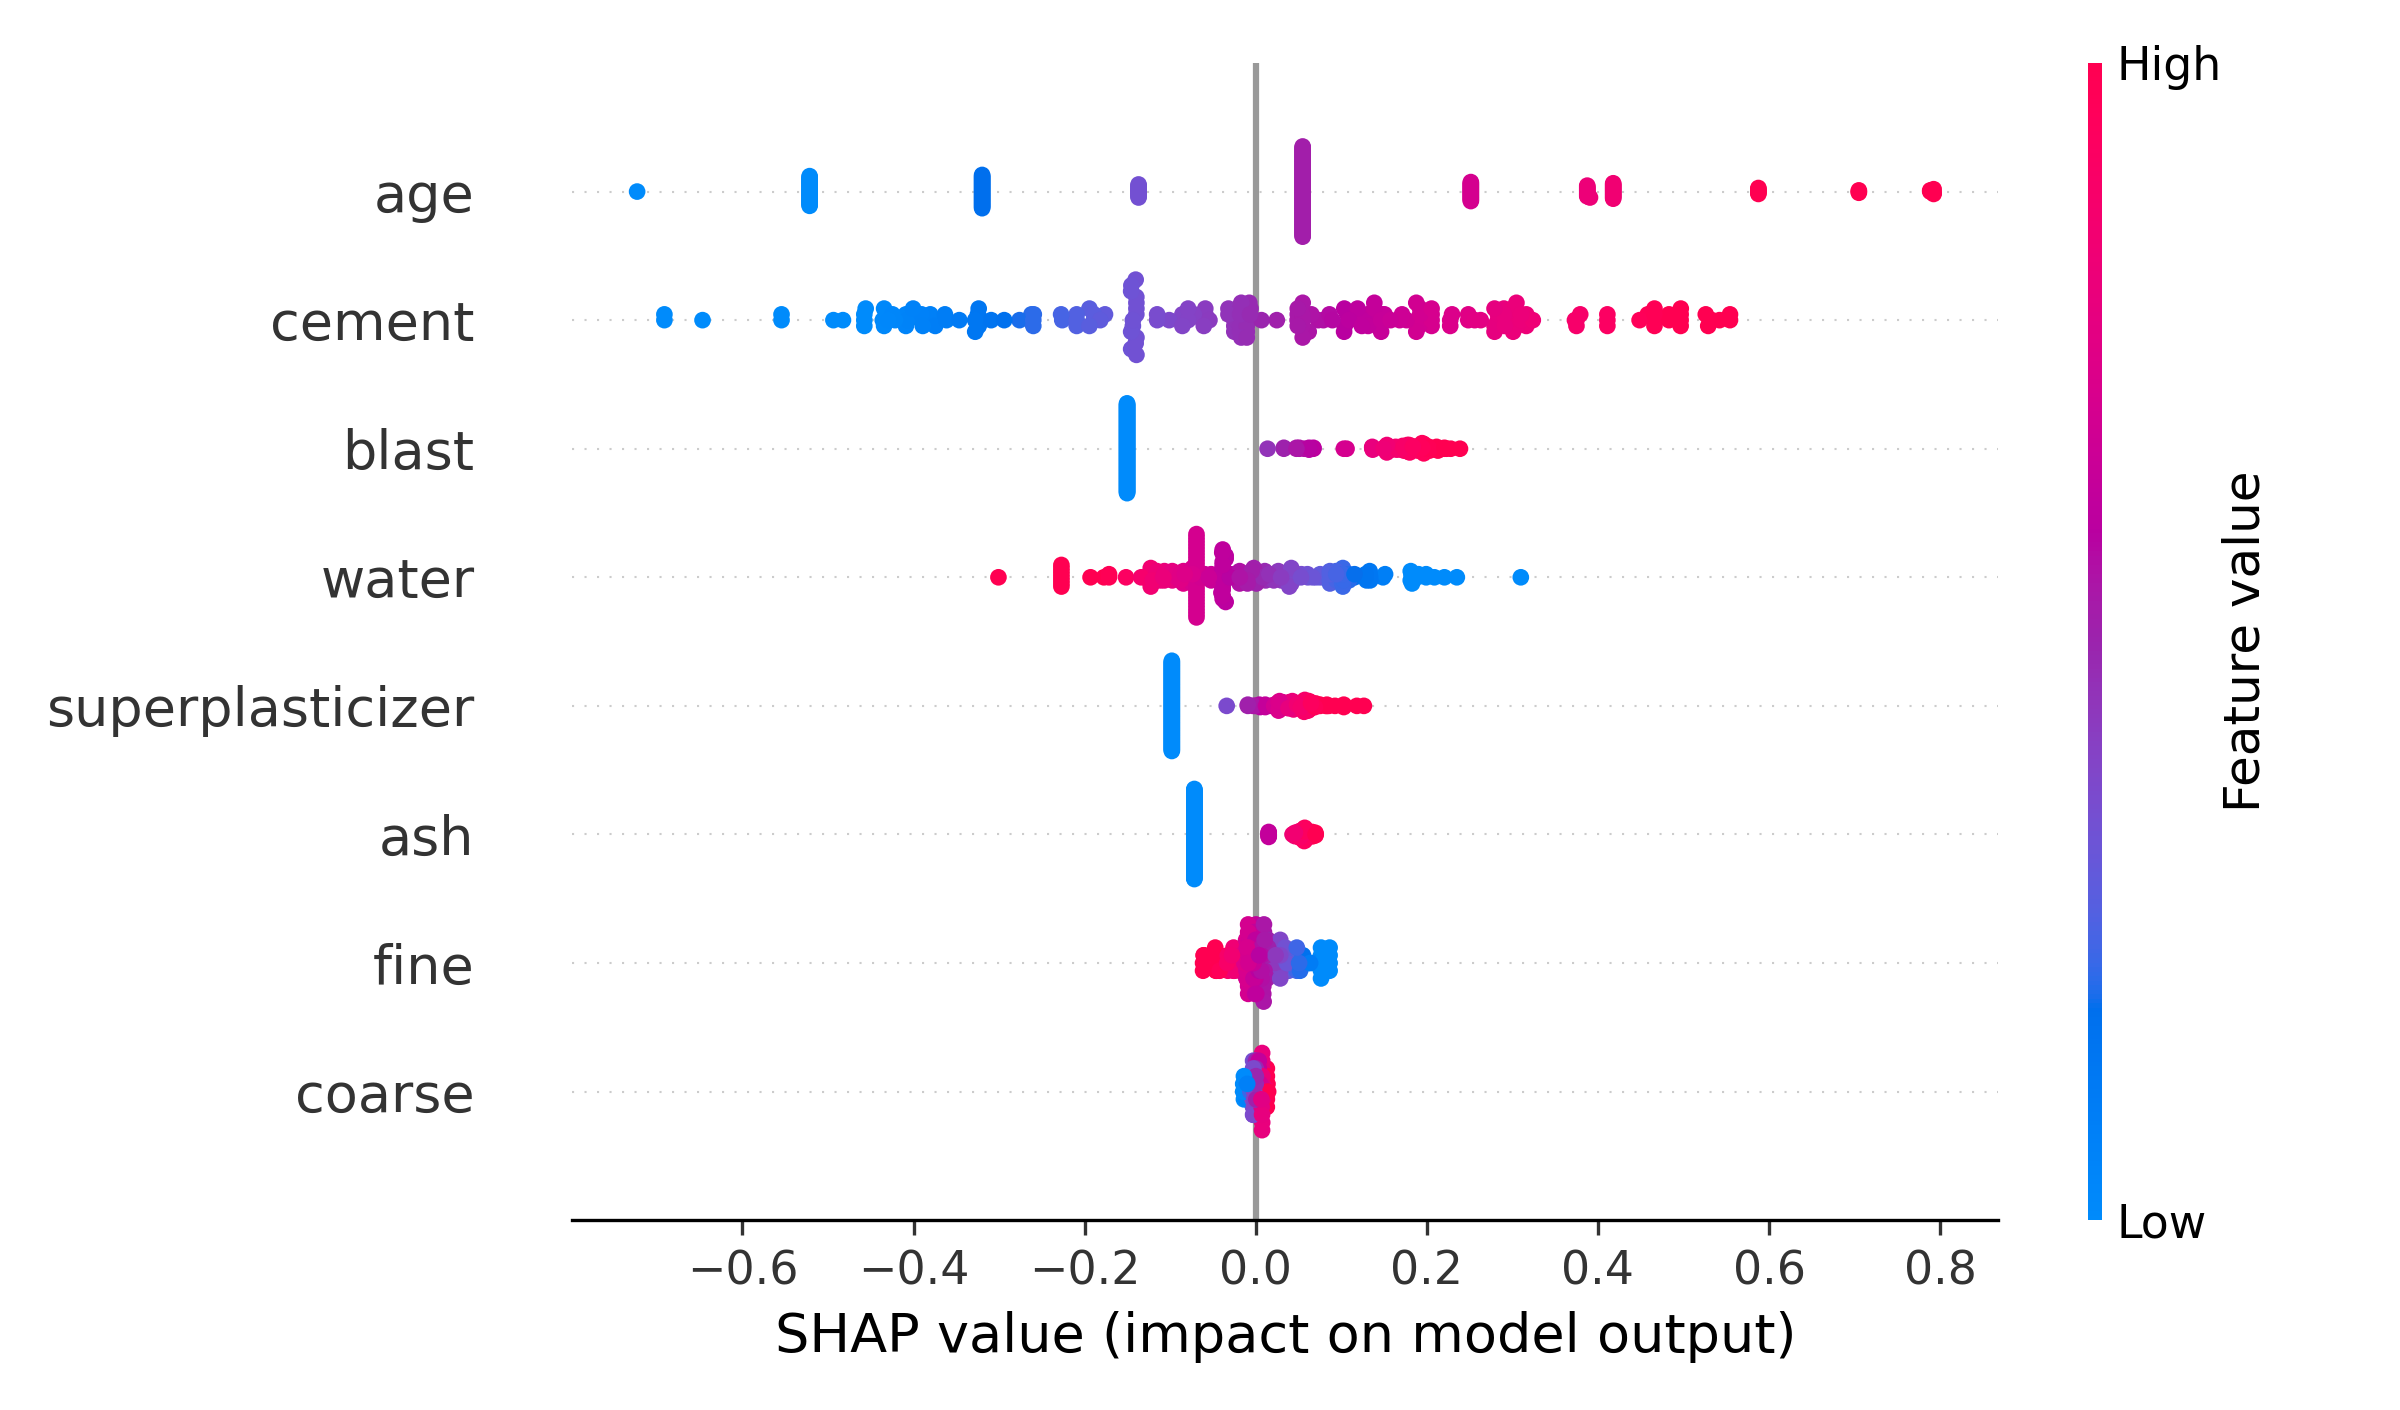
\includegraphics[width=1\textwidth]{../scripts/images/shap_beeswarm_plot.png}
    Quelle: Eigene Darstellung, \ref{linreg}.
    \label{pic:shap_beeswarm}
\end{figure}

Der SHAP Beeswarm Plot in Abbildung \ref{pic:shap_beeswarm} bietet eine globale 
Sicht auf die Modellvorhersagen, indem er die Verteilung der SHAP-Werte für jedes Merkmals 
über alle Beobachtungen hinweg darstellt. Jeder Punkt repräsentiert eine Beobachtung aus dem Datensatz.
Die Farbe der Punkte zeigt die Merkmalsausprägungen an: hohe Werte in Rot und niedrige Werte in Blau. 
Die Position auf der x-Achse gibt den Einfluss des Merkmals auf die Modellvorhersage an. 
Positive SHAP-Werte (rechts von der Nulllinie) zeigen eine Erhöhung der Vorhersage an, 
während negative Werte (links von der Nulllinie) eine Verringerung bedeuten. 

Das Merkmal age zeigt eine hohe Variabilität in seinem Einfluss auf die Modellvorhersage. 
Höhere Werte von age sind mit einer Zunahme der Vorhersage (positive SHAP-Werte) assoziiert, 
was durch die rechtsseitigen Punkte in der Grafik dargestellt wird. 
Niedrigere Werte führen hingegen zu einer geringeren Vorhersage, 
erkennbar an den linksseitigen Punkten. Diese Streuung der Punkte zeigt, 
dass die Auswirkung von age auf die Vorhersage stark von seiner quantitativen Ausprägung abhängt.

Diese Darstellung ermöglicht es, die Merkmale zu identifizieren, 
die den größten Einfluss auf das Modell haben und wie dieser Einfluss über 
unterschiedliche Beobachtungen variiert.

\begin{figure}[!h]
    \caption{SHAP Bar Plot}
    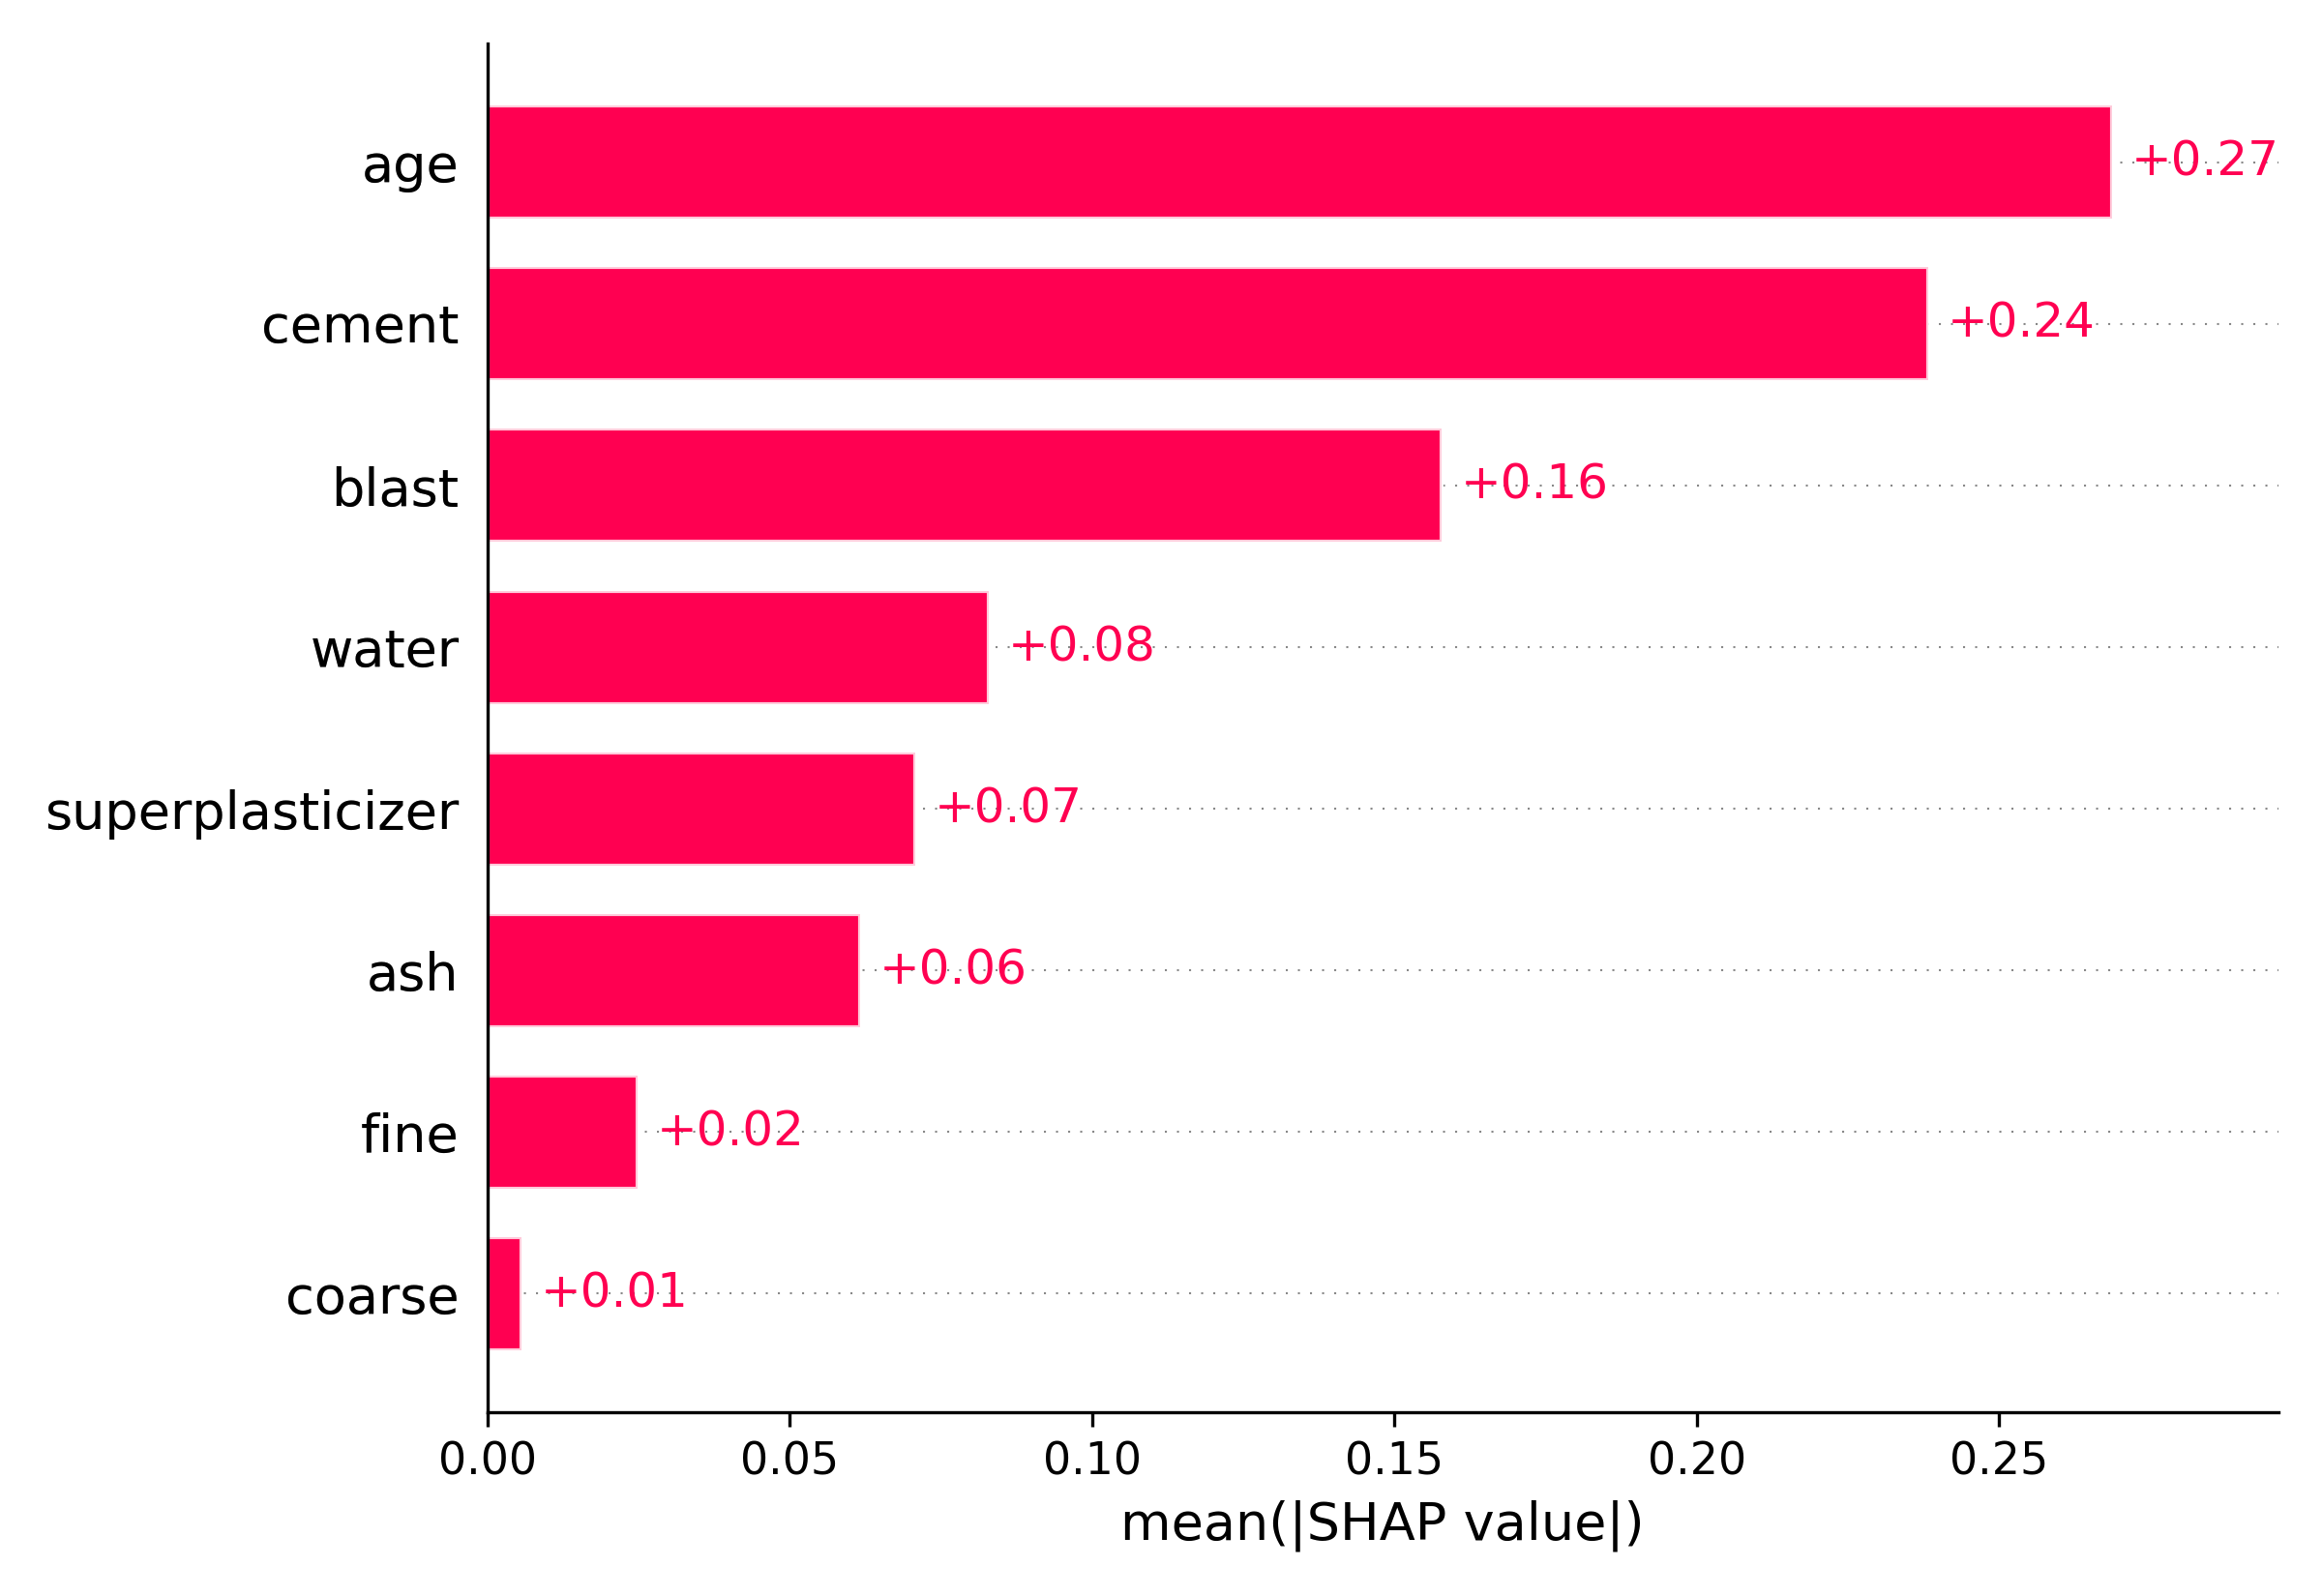
\includegraphics[width=1\textwidth]{../scripts/images/shap_bar_plot.png}
    Quelle: Eigene Darstellung, \ref{linreg}.
    \label{pic:shap_bar}
\end{figure}

Der SHAP Bar Plot in Abbildung \ref{pic:shap_bar} illustriert die durchschnittliche 
Auswirkung jedes Merkmals auf das Modell, gemessen an der absoluten Größe der SHAP-Werte 
über alle Beobachtungen hinweg. Die Balken zeigen die durchschnittlichen Beiträge der 
Merkmale zur Vorhersage: Je länger der Balken, desto größer ist der Einfluss des jeweiligen Merkmals. 
Hier ist das Merkmal age mit dem höchsten durchschnittlichen SHAP-Wert (+0.27) das einflussreichste 
Merkmal, was auf eine starke positive Beziehung zur Zielvariablen hinweist. Die weiteren Merkmale 
folgen in absteigender Reihenfolge ihrer Bedeutung.

Es fällt auf, dass eine Übereinstimmung in der Reihenfolge der Merkmalsrelevanz zwischen 
der Permutation Feature Importance aus Abbildung \ref{pic:permutation} und den SHAP-Werten aus Abbildung \ref{pic:shap_bar}
besteht, obwohl die zugrundeliegenden Interpretationen dieser beiden Methoden deutlich verschieden sind. 

Die Permutation Feature Importance konzentriert sich darauf, die Veränderungen im Vorhersagefehler des Modells, 
speziell den mittleren quadratischen Fehler, zu messen, die eintreten, wenn die Werte eines Merkmals zufällig vertauscht werden. 
Diese Methode gibt Aufschluss darüber, wie stark das Modell auf das jeweilige Merkmal für seine Vorhersagegenauigkeit angewiesen ist. 
Ein wesentliches Merkmal dieser Methode ist, dass sie nicht direkt die Wechselwirkungen zwischen den Merkmalen berücksichtigt. 
Sie zeigt vielmehr, wie wichtig ein Merkmal isoliert für die Gesamtleistung des Modells ist.

Im Gegensatz dazu bieten die SHAP-Werte einen tieferen Einblick in die Beiträge jedes Merkmals zur Vorhersageleistung des Modells. 
Sie quantifizieren den Einfluss eines Merkmals auf die Abweichung der Prognose vom Basiswert, also der durchschnittlichen Vorhersage des Modells. 
Hierbei wird nicht nur die individuelle Wichtigkeit jedes Merkmals hervorgehoben, sondern auch deren Wechselwirkungen mit anderen 
Merkmalen berücksichtigt. Diese Methodik ermöglicht es, sowohl eine globale als auch eine lokale Perspektive auf die Modellvorhersagen zu werfen. 
Während die globale Interpretation durchschnittliche Auswirkungen aller Merkmale aufzeigt, erlaubt die lokale Sichtweise, die Vorhersagen 
für einzelne Beobachtungen präzise zu erklären.

Diese unterschiedlichen Herangehensweisen und Interpretationen der Merkmalsrelevanz, einerseits durch die 
Permutation Feature Importance und andererseits durch die SHAP-Werte, verdeutlichen die Komplexität und die Tiefe der Analyse, 
die für ein umfassendes Verständnis von Vorhersagemodellen erforderlich ist. Beide Methoden ergänzen sich gegenseitig und tragen dazu bei, 
ein vollständigeres Bild der Dynamiken innerhalb des Modells zu zeichnen.

Shapley-Werte bieten für die Prognose der Druckfestigkeit von Beton einen signifikanten Vorteil, 
da sie eine gerechte Verteilung des Vorhersagebeitrags über alle Merkmale gewährleisten. 
Diese gerechte Verteilung ist eine der Kernstärken der 
Shapley-Werte, die sie von anderen Methoden abhebt.

Die Druckfestigkeit von Beton ist das Ergebnis einer komplexen Interaktion verschiedener 
Materialkomponenten und Eigenschaften wie Zementgehalt, Wasser-Zement-Verhältnis, 
Zuschlagstoffe und Alter des Betons. Jede dieser Komponenten trägt unterschiedlich 
zur Endfestigkeit bei, und ihre Effekte können nicht isoliert betrachtet werden, 
da sie interdependent sind. Hier ermöglichen Shapley-Werte eine faire und ausgewogene 
Zurechnung der Einflüsse jedes Merkmals auf die Vorhersage, indem sie die marginalen 
Beiträge jedes Merkmals unter Berücksichtigung aller möglichen Kombinationen von Merkmalen 
im Modell kalkulieren.

Andere Methoden, wie beispielsweise die Betrachtung von Regressionskoeffizienten, 
geben zwar Aufschluss über die Richtung und Stärke des Zusammenhangs zwischen Merkmalen 
und der Zielvariable, vernachlässigen jedoch die Interaktionseffekte zwischen den Merkmalen.

In der Praxis bedeutet dies für die Prognose der Druckfestigkeit von Beton, 
dass Shapley-Werte eine präzise Zuordnung der Einflussstärke jedes Bestandteils 
und Verarbeitungsmerkmals erlauben. Da die Festigkeit von Beton von einer Vielzahl von 
Faktoren abhängt, ermöglicht die granulare Aufschlüsselung der Shapley-Werte eine 
detailreiche Einsicht, welche Komponenten optimiert werden sollten, um die gewünschten 
Eigenschaften des Betons zu erreichen.

Im Kontext von industriellen Anwendungen und Forschung, wo Entscheidungen auf Grundlage 
der Modellvorhersagen getroffen werden, gewährleisten Shapley-Werte somit eine transparente 
und gerechtfertigte Grundlage. Dies ist nicht nur für die Entwicklung von Betonmischungen 
von Bedeutung, sondern auch für die Einhaltung von Bauvorschriften und die Gewährleistung 
der Sicherheit. Durch die Verwendung von Shapley-Werten kann die Forschung im Bereich 
der Materialwissenschaften fundierter und zielgerichteter gestaltet werden, was zu einer 
effizienteren und effektiveren Materialentwicklung führt.

Im abschließenden Kapitel dieser Arbeit werden die wichtigsten Erkenntnisse zusammengefasst 
und diskutiert.


\chapter{Fazit}

Diese Arbeit hat die Anwendung und Interpretation von SHAP-Werten in der 
linearen Regressionsanalyse zur Vorhersage der Druckfestigkeit von Beton umfassend untersucht. 
SHAP-Werte, als ein fortschrittlicher Ansatz zur Modellinterpretation, haben sich als besonders 
wertvoll erwiesen, indem sie eine tiefere und nuanciertere Einsicht in die Beiträge einzelner 
Merkmale zur Modellvorhersage bieten. Im Vergleich zu herkömmlichen Interpretationsmethoden, 
wie der Analyse der Regressionskoeffizienten und der Permutation der Merkmalrelevanz, 
bieten SHAP-Werte mehrere Vorteile.

Einer der Hauptvorteile von SHAP-Werten liegt in ihrer Fähigkeit, sowohl globale als auch 
lokale Interpretationen zu ermöglichen. Sie erlauben es, den Einfluss einzelner Merkmale auf 
spezifische Vorhersagen zu verstehen, während gleichzeitig ein Überblick über deren Bedeutung 
im gesamten Modell gegeben wird. Darüber hinaus berücksichtigen SHAP-Werte die Interaktionen 
zwischen den Merkmalen und bieten somit eine ganzheitliche Sicht auf die Modellvorhersagen. 
Dies ist besonders relevant in komplexen Datenstrukturen, wo Merkmalsinteraktionen eine signifikante
Rolle spielen.

Ein weiterer zentraler Vorteil der SHAP-Werte liegt in ihrer umfassenden Erklärungskraft.
Im Gegensatz zur Permutation der Merkmalrelevanz, die sich darauf konzentriert, wie sich der 
Vorhersagefehler des Modells verändert, wenn die Werte eines Merkmals zufällig vertauscht werden, 
bieten SHAP-Werte eine detaillierte Aufschlüsselung des Beitrags jedes einzelnen Merkmals zur 
Vorhersage. Diese Eigenschaft der SHAP-Werte ist von Vorteil, da sie eine faire 
Aufteilung der Vorhersageabweichung unter allen Merkmalsausprägungen gewährleistet – bekannt 
als die Effizienzeigenschaft der Shapley-Werte. Diese faire Aufteilung ist dann wichtig, 
wenn eine vollständige und transparente Erklärbarkeit erforderlich ist.

Trotz dieser Stärken ist es wichtig, auch die Grenzen der SHAP-Methode zu erkennen. 
Eine der Herausforderungen bei der Anwendung von SHAP-Werten ist die Interpretation der Ergebnisse, 
insbesondere wenn es um komplexe Modelle mit einer großen Anzahl von Merkmalen und komplizierten 
Interaktionen geht. Die Interpretation kann schnell überwältigend werden und erfordert ein tiefes 
Verständnis der zugrundeliegenden Daten und des Modells. Darüber hinaus kann die Berechnung von 
SHAP-Werten insbesondere bei großen Datensätzen rechenintensiv sein, was praktische Einschränkungen 
mit sich bringt.

Ein Nachteil ist die potenzielle Verzerrung, die durch die Stichprobenabhängigkeit 
der SHAP-Werte entstehen kann. SHAP-Werte basieren auf der Annahme, dass die Daten, auf denen
das Modell trainiert wurde, repräsentativ für die zugrunde liegende Population sind. 
Wenn diese Annahme nicht erfüllt ist, können die SHAP-Werte irreführende Interpretationen liefern.

Zusammenfassend lässt sich sagen, dass SHAP-Werte eine bedeutende Erweiterung der Möglichkeiten
zur Interpretation von linearen Modellen darstellen. Sie bieten tiefergehende Einblicke in die 
Funktionsweise von linearen Modellen und ermöglichen eine präzisere und umfassendere Analyse der Merkmalsrelevanz 
und -interaktionen. Dennoch ist es entscheidend, ihre Limitationen zu verstehen und sie als 
einen Teil eines umfassenden Prozesses der Modellinterpretation und -validierung zu betrachten. 

% Schalgwortverzeichnis (Index)
%\printindex

% Literaturverzeichnis
%\nocite{*}
\bibliographystyle{alphaurl}
\cleardoublepage
\phantomsection
\addcontentsline{toc}{chapter}{Literaturverzeichnis}
\bibliography{bibtex.bib}
\cleardoubleemptypage

% Abbildungsverzeichnis einbinden und ins Inhaltsverzeichnis
% WORKAROUND: tocloft und KOMA funktionieren zusammen nicht
% korrekt\phantomsection
\phantomsection 
\addcontentsline{toc}{chapter}{\listfigurename} 
\listoffigures
\cleardoubleemptypage

% Tabellenverzeichnis einbinden und ins Inhaltsverzeichnis
% WORKAROUND: tocloft und KOMA funktionieren zusammen nicht
% korrekt\phantomsection
\phantomsection
\addcontentsline{toc}{chapter}{\listtablename}
\listoftables
\cleardoubleemptypage

% Quellcodeverzeichnis einbinden und ins Inhaltsverzeichnis
\phantomsection
\addcontentsline{toc}{chapter}{Quellcodeverzeichnis}

%Define listing
\makeatletter
\begingroup\let\newcounter\@gobble\let\setcounter\@gobbletwo
  \globaldefs\@ne \let\c@loldepth\@ne
  \newlistof{listings}{lol}{\lstlistlistingname}
\endgroup
\let\l@lstlisting\l@listings
\makeatother
\setlength{\cftlistingsindent}{0em}
\renewcommand{\cftlistingsafterpnum}{\vskip0pt} %Spacing between entries
\renewcommand*{\cftlistingspresnum}{\lstlistingname~}
\settowidth{\cftlistingsnumwidth}{\cftlistingspresnum}
\renewcommand{\lstlistlistingname}{Quellcodeverzeichnis}
% Tabellenverzeichnis anpassen
\renewcommand{\lstlistingname}{Codeauschnitt}
\renewcommand{\cftlistingsaftersnum}{:}
% Breite des Nummerierungsbereiches [Codeauschnitt 1:]
\newlength{\codeLength}
\settowidth{\codeLength}{\bfseries\lstlistingname\cftlistingsaftersnum}
\addtolength{\codeLength}{5mm}
\setlength{\cftlistingsnumwidth}{\codeLength}
\lstlistoflistings
\cleardoubleemptypage


% Eidesstattliche Erklärung
\chapter*{Eidesstattliche Erklärung\markboth{Eidesstattliche Erklärung}{}}
% Eintrag in das Inhaltsverzeichnis 
\addcontentsline{toc}{chapter}{Eidesstattliche Erklärung}

Ich versichere an Eides statt, dass ich die vorstehende Arbeit selbständig 
und ohne fremde Hilfe angefertigt und mich anderer als der im beigefügten 
Verzeichnis angegebenen Hilfsmittel nicht bedient habe. Alle Stellen, die wörtlich oder sinngemäß aus Veröffentlichungen 
übernommen wurden, sind als solche kenntlich gemacht. Alle Internetquellen sind der Arbeit beigefügt. 

Des Weiteren versichere ich, dass ich die Arbeit vorher nicht in 
einem anderen Prüfungsverfahren eingereicht habe und dass die eingereichte 
schriftliche Fassung der auf dem elektronischen Speichermedium entspricht.


\vspace*{1.5cm} \par
\docOrt, den \docAbgabedatum
\vspace{1cm}


\noindent\rule[0cm]{5cm}{0.5pt}\\
\textsc{\docVorname~\docNachname}


%Zurücksetzen \chaptermark
\let\chaptermark\oldchaptermark

% Hier können Anhaenge angefuegt werden
\begin{appendices}
\chapter{Quellcode}

\section{requirements.txt}
\lstinputlisting[language=python,label=requirements, nolol]{../scripts/requirements.txt}

\section{charts.py}
\lstinputlisting[language=Python,label=charts, nolol]{../scripts/charts.py}

\section{linreg.py}
\lstinputlisting[language=Python,label=linreg, nolol]{../scripts/linreg.py}

\end{appendices}
\end{document} 
 